\subsubsection{UC1 Caso d'uso pubblico}
\begin{figure}[H]
\centering
\noindent\makebox[\textwidth]{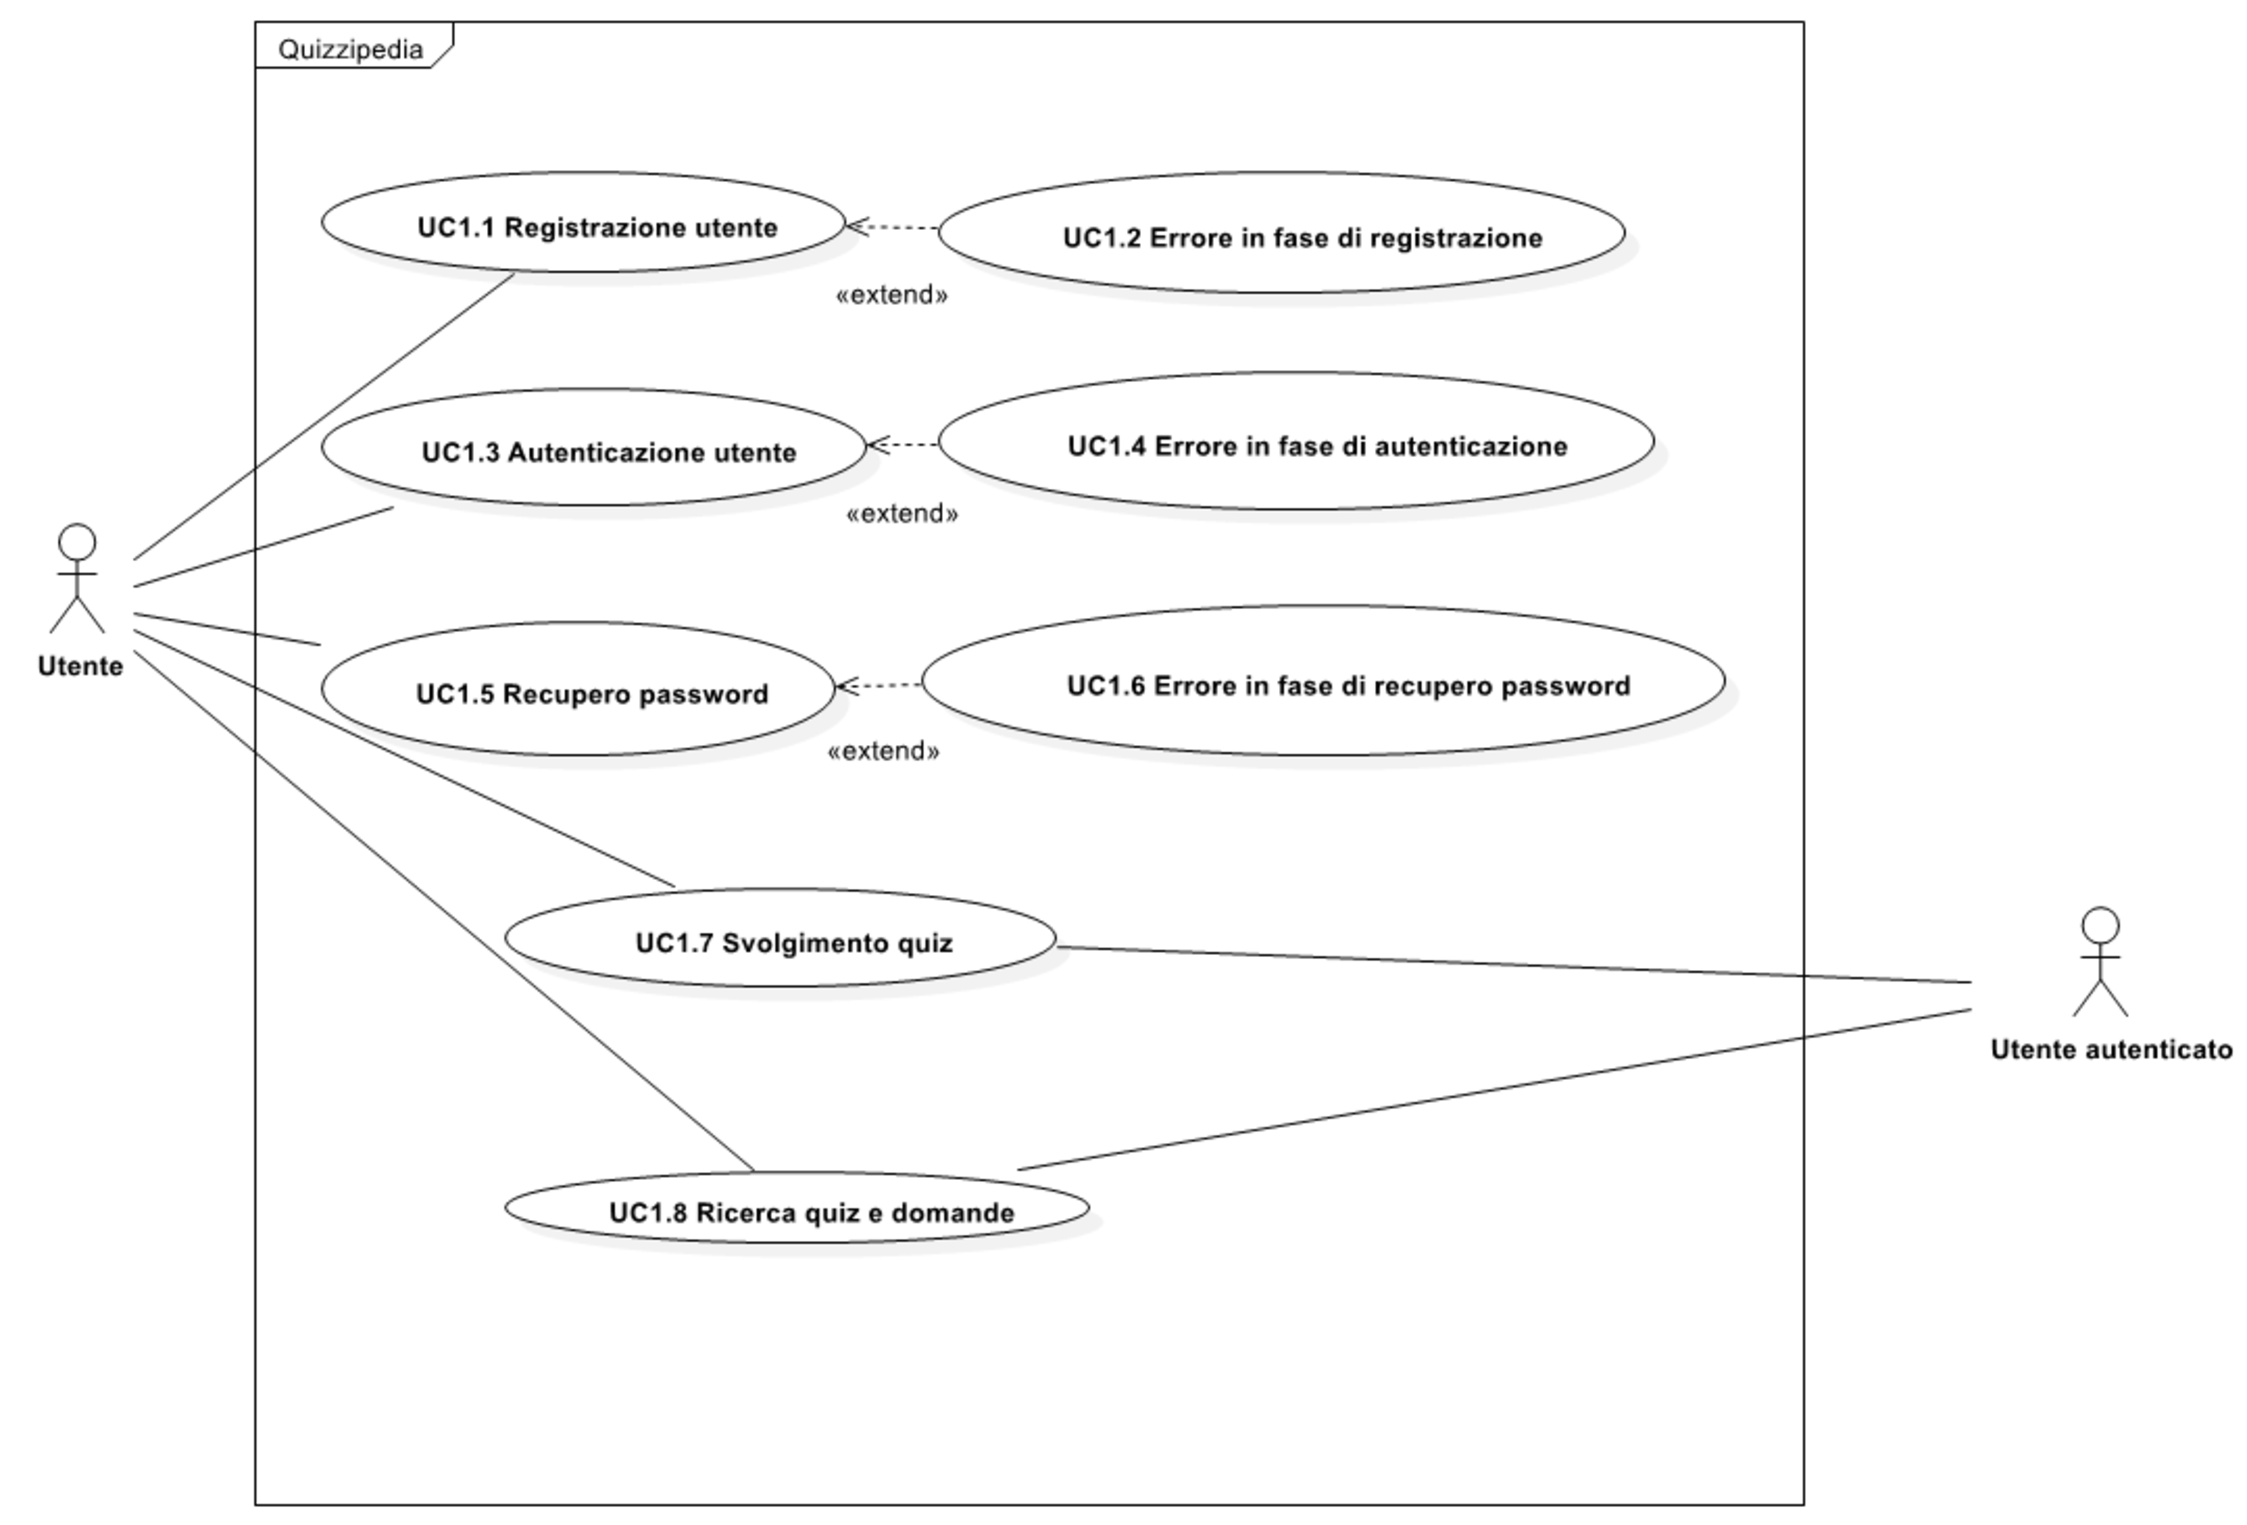
\includegraphics[width=\textwidth]{Img/UC Caso d'uso pubblico.pdf}}
\caption{UC1 Caso d'uso pubblico}
\end{figure}
\begin{itemize}
\item \textbf{Attori}: Utente, Utente Autenticato.
\item \textbf{Scenario principale}:
\begin{enumerate}
\item Registrazione utente (UC1.1);
\item Errore in fase di registrazione (UC1.2);
\item Autenticazione utente (UC1.3);
\item Errore in fase di autenticazione (UC1.4);
\item Recupero password (UC1.5);
\item Errore in fase di recupero password (UC1.6);
\item Svolgimento quiz (UC1.7);
\item Ricerca quiz e domande (UC1.8);
\item Interruzione volontaria della registrazione (UC1.9);
\item Interruzione volontaria dell'autenticazione (UC1.10);
\item Interruzione volontaria dello svolgimento del quiz (UC1.11);
\item Interruzione volontaria della ricerca (UC1.12);
\item Interruzione volontaria del recupero password (UC1.13).
\end{enumerate}
\item \textbf{Descrizione}: l'utente accede al sito. Può effettuare la registrazione, autenticarsi nel sistema, effettuare il recupero della propria password, cercare quiz e domande, svolgere quiz.
\item \textbf{Precondizione}: l'utente si è connesso al sito web di Quizzipedia attraverso un browser supportato.
\item \textbf{Postcondizione}: l'utente ha scelto l'operazione da intraprendere.
\end{itemize}
\subsubsection{UC1.1 Registrazione utente}
\begin{figure}[H]
\centering
\noindent\makebox[\textwidth]{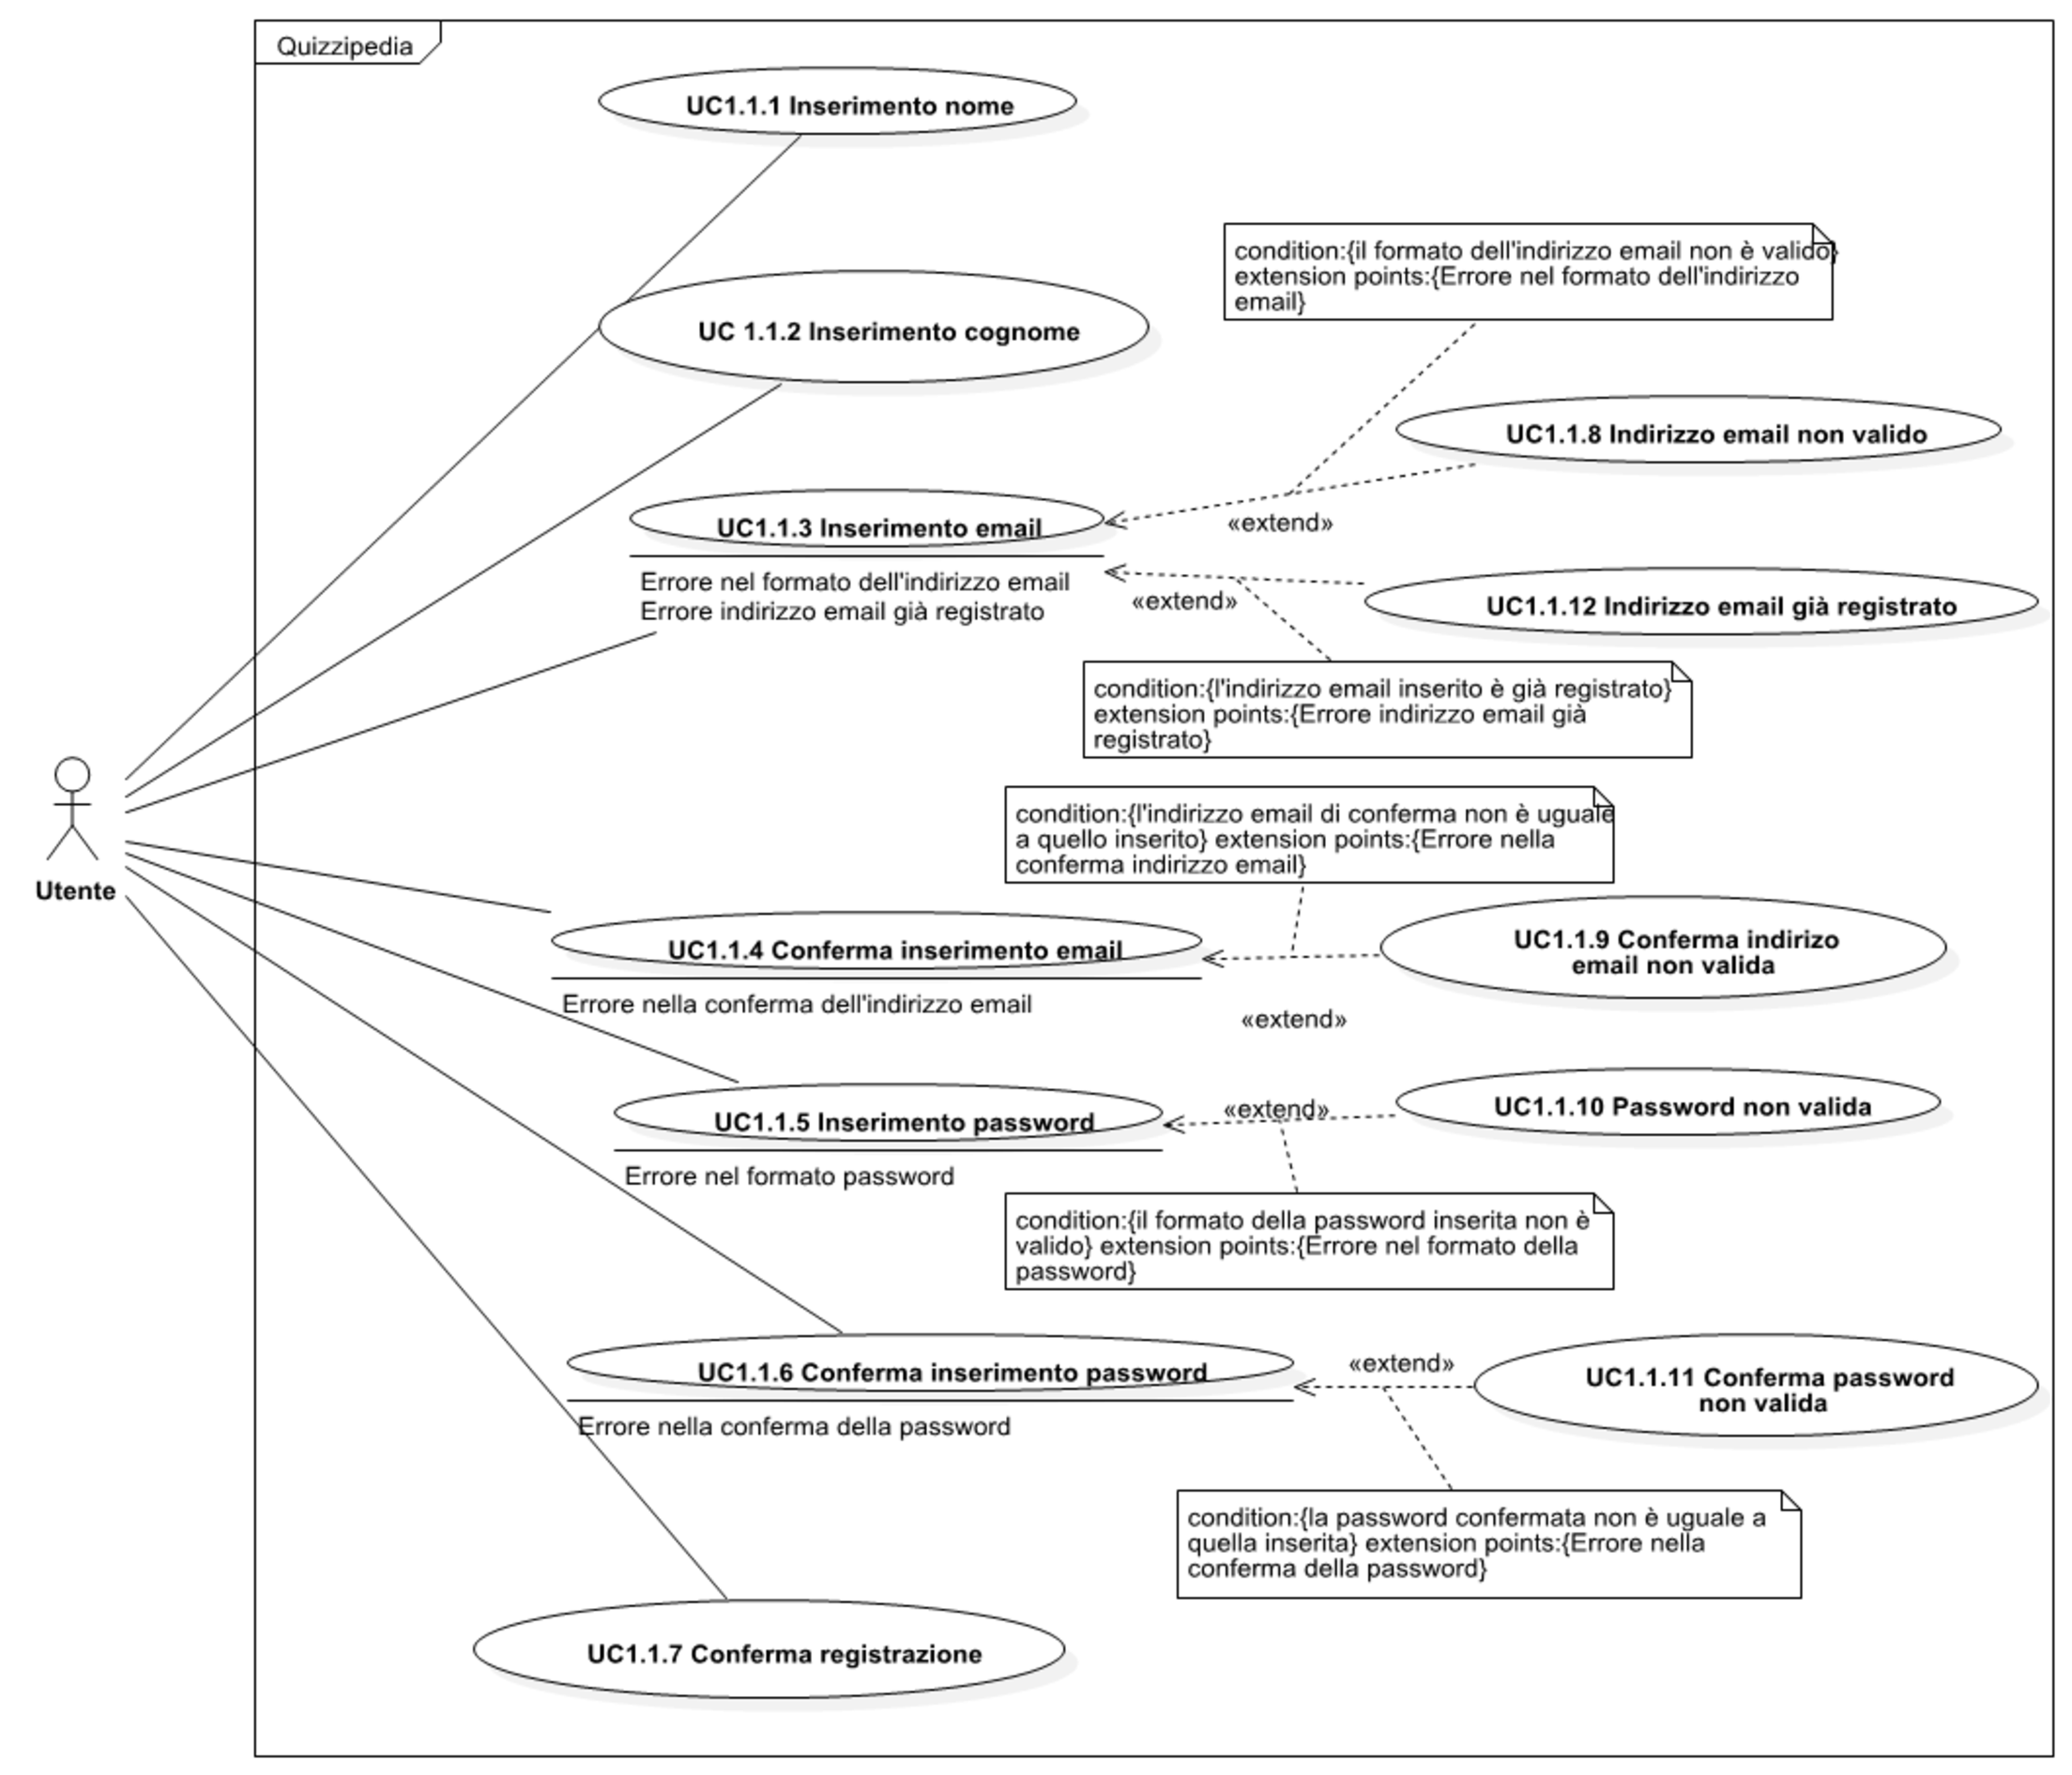
\includegraphics[width=\textwidth]{Img/UC Registrazione utente.pdf}}
\caption{UC1.1 Registrazione utente}
\end{figure}
\begin{itemize}
\item \textbf{Attori}: Utente.
\item \textbf{Scenario principale}:
\begin{enumerate}
\item Inserimento nome (UC1.1.1);
\item Inserimento cognome (UC1.1.2);
\item Inserimento email (UC1.1.3);
\item Conferma inserimento email (UC1.1.4);
\item Inserimento password (UC1.1.5);
\item Conferma inserimento password (UC1.1.6);
\item Conferma registrazione (UC1.1.7);
\item Indirizzo email non valido (UC1.1.8);
\item Conferma indirizzo email non valida (UC1.1.9);
\item Password non valida (UC1.1.10);
\item Conferma password non valida (UC1.1.11);
\item Indirizzo email già registrato (UC1.1.12).
\end{enumerate}
\item \textbf{Estensioni}:
\begin{itemize}
\item Errore in fase di registrazione (UC1.2);
\item Interruzione volontaria della registrazione (UC1.9).
\end{itemize}
\item \textbf{Descrizione}: l'utente crea un account Quizzipedia per poter usufruire delle funzionalità offerte dal sistema agli utenti registrati.
\item \textbf{Precondizione}: l'utente si è connesso al sito web di Quizzipedia attraverso un browser supportato e ha scelto di effettuare la registrazione.
\item \textbf{Postcondizione}: l'utente è stato registrato nel sistema con i dati immessi.
\end{itemize}
\subsubsection{UC1.1.1 Inserimento nome}
\begin{itemize}
\item \textbf{Attori}: Utente.
\item \textbf{Scenario principale}: l'utente inserisce il proprio nome.
\item \textbf{Descrizione}: per portare a termine la registrazione, l'utente deve inserire il proprio nome.
\item \textbf{Precondizione}: l'utente si trova nella pagina di registrazione e deve ancora inserire il proprio nome.
\item \textbf{Postcondizione}: l'utente ha inserito il nome.
\end{itemize}
\subsubsection{UC1.1.2 Inserimento cognome}
\begin{itemize}
\item \textbf{Attori}: Utente.
\item \textbf{Scenario principale}: l'utente inserisce il proprio cognome.
\item \textbf{Descrizione}: per portare a termine la registrazione, l'utente deve inserire il proprio cognome.
\item \textbf{Precondizione}: l'utente si trova nella pagina di registrazione e deve ancora inserire il proprio cognome.
\item \textbf{Postcondizione}: l'utente ha inserito il cognome.
\end{itemize}
\subsubsection{UC1.1.3 Inserimento email}
\begin{itemize}
\item \textbf{Attori}: Utente.
\item \textbf{Scenario principale}: l'utente inserisce il proprio indirizzo email.
\item \textbf{Estensioni}:
\begin{itemize}
\item Indirizzo email non valido (UC1.1.8).
\end{itemize}
\item \textbf{Descrizione}: per portare a termine la registrazione, l'utente deve inserire il proprio indirizzo email.
\item \textbf{Precondizione}: l'utente si trova nella pagina di registrazione e deve ancora inserire l'indirizzo email.
\item \textbf{Postcondizione}: l'utente ha inserito un indirizzo email valido.
\end{itemize}
\subsubsection{UC1.1.4 Conferma inserimento email}
\begin{itemize}
\item \textbf{Attori}: Utente.
\item \textbf{Scenario principale}: l'utente conferma l'inserimento del proprio indirizzo email.
\item \textbf{Estensioni}:
\begin{itemize}
\item Conferma indirizzo email non valida (UC1.1.9).
\end{itemize}
\item \textbf{Descrizione}: per portare a termine la registrazione, l'utente deve confermare il proprio indirizzo email.
\item \textbf{Precondizione}: l'utente si trova nella pagina di registrazione, ha inserito l'indirizzo email e deve ancora confermarlo.
\item \textbf{Postcondizione}: l'utente ha confermato un indirizzo email valido e uguale a quello inserito.
\end{itemize}
\subsubsection{UC1.1.5 Inserimento password}
\begin{itemize}
\item \textbf{Attori}: Utente.
\item \textbf{Scenario principale}: l'utente inserisce la propria password.
\item \textbf{Estensioni}:
\begin{itemize}
\item Password non valida (UC1.1.10).
\end{itemize}
\item \textbf{Descrizione}: per portare a termine la registrazione, l'utente deve inserire la propria password.
\item \textbf{Precondizione}: l'utente si trova nella pagina di registrazione e deve ancora inserire la password.
\item \textbf{Postcondizione}: l'utente ha inserito una password valida.
\end{itemize}
\subsubsection{UC1.1.6 Conferma inserimento password}
\begin{itemize}
\item \textbf{Attori}: Utente.
\item \textbf{Scenario principale}: l'utente conferma l'inserimento della propria password.
\item \textbf{Estensioni}:
\begin{itemize}
\item Conferma password non valida (UC1.1.11).
\end{itemize}
\item \textbf{Descrizione}: per portare a termine la registrazione, l'utente deve confermare la propria password.
\item \textbf{Precondizione}: l'utente si trova nella pagina di registrazione, ha inserito la password e deve ancora confermarla.
\item \textbf{Postcondizione}: l'utente ha confermato una password valida e uguale a quella inserita.
\end{itemize}
\subsubsection{UC1.1.7 Conferma registrazione}
\begin{itemize}
\item \textbf{Attori}: Utente.
\item \textbf{Scenario principale}: l'utente conferma la registrazione.
\item \textbf{Descrizione}: per portare a termine la registrazione, l'utente deve confermare i dati precedentemente inseriti.
\item \textbf{Precondizione}: l'utente si trova in una pagina del sito web che gli permette di confermare i dati precedentemente inseriti.
\item \textbf{Postcondizione}: L'utente ha scelto di continuare la registrazione con i dati immessi.
\end{itemize}
\subsubsection{UC1.1.8 Indirizzo email non valido}
\begin{itemize}
\item \textbf{Attori}: Utente.
\item \textbf{Scenario principale}: l'utente inserisce nuovamente l'indirizzo email.
\item \textbf{Descrizione}: l'indirizzo email non è valido e deve essere inserito nuovamente.
\item \textbf{Precondizione}: L'utente sta effettuando la registrazione e ha inserito un indirizzo email non valido.
\item \textbf{Postcondizione}: L'utente ha visualizzato un messaggio di errore che indica che l'indirizzo email inserito non è valido.
\end{itemize}
\subsubsection{UC1.1.9 Conferma indirizzo email non valida}
\begin{itemize}
\item \textbf{Attori}: Utente.
\item \textbf{Scenario principale}: l'utente conferma nuovamente l'indirizzo email.
\item \textbf{Descrizione}: l'indirizzo email non è uguale a quello precedentemente inserito.
\item \textbf{Precondizione}: L'utente sta effettuando la registrazione e ha confermato l'indirizzo email in modo errato.
\item \textbf{Postcondizione}: L'utente ha visualizzato un messaggio di errore che indica che l'indirizzo email confermato non è uguale a quello precedentemente inserito.
\end{itemize}
\subsubsection{UC1.1.10 Password non valida}
\begin{itemize}
\item \textbf{Attori}: Utente.
\item \textbf{Scenario principale}: l'utente inserisce nuovamente la password.
\item \textbf{Descrizione}: la password inserita non è valida e quindi deve essere inserita nuovamente.
\item \textbf{Precondizione}: l'utente si trova nella pagina di registrazione e ha inserito una password non valida.
\item \textbf{Postcondizione}: l'utente ha visualizzato un messaggio di errore che indica che la password inserita non è valida.
\end{itemize}
\subsubsection{UC1.1.11 Conferma password non valida}
\begin{itemize}
\item \textbf{Attori}: Utente.
\item \textbf{Scenario principale}: l'utente conferma la password nuovamente.
\item \textbf{Descrizione}: la password non è uguale a quella precedentemente inserita.
\item \textbf{Precondizione}: l'utente si trova nella pagina di registrazione e ha confermato la password in maniera errata.
\item \textbf{Postcondizione}: l'utente ha visualizzato un messaggio di errore che indica che la password confermata non è uguale a quella precedentemente inserita.
\end{itemize}
\subsubsection{UC1.1.12 Indirizzo email già registrato}
\begin{itemize}
\item \textbf{Attori}: Utente.
\item \textbf{Scenario principale}: l'utente inserisce nuovamente l'indirizzo email.
\item \textbf{Descrizione}: l'indirizzo email inserito è già registrato.
\item \textbf{Precondizione}: l'utente sta effettuando la registrazione e ha inserito un indirizzo email già registrato.
\item \textbf{Postcondizione}: L'utente ha visualizzato un messaggio di errore che indica che l'indirizzo email inserito è già registrato.
\end{itemize}
\subsubsection{UC1.2 Errore in fase di registrazione}
\begin{itemize}
\item \textbf{Attori}: Utente.
\item \textbf{Scenario principale}: l'utente visualizza il messaggio di errore.
\item \textbf{Descrizione}: l'utente visualizza un messaggio di errore che lo avvisa che il tentativo di autenticazione non è andato a buon termine.
\item \textbf{Precondizione}: si è verificata una delle seguenti condizioni: l'indirizzo email inserito non è associato a un account registrato, oppure la combinazione di indirizzo email e password immessa è errata.
\item \textbf{Postcondizione}: l'utente ha visualizzato il messaggio di errore.
\end{itemize}
\subsubsection{UC1.3 Autenticazione utente}
\begin{figure}[H]
\centering
\noindent\makebox[\textwidth]{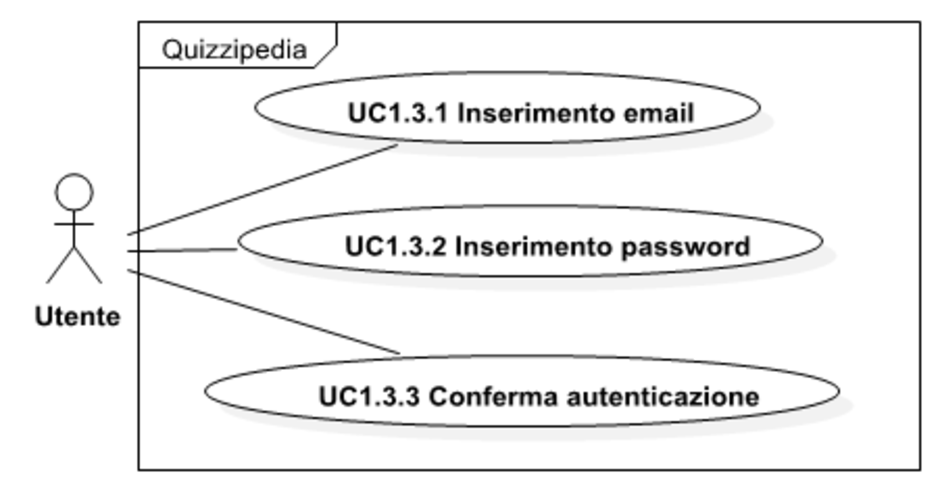
\includegraphics[width=\textwidth]{Img/UC Autenticazione utente.pdf}}
\caption{UC1.3 Autenticazione utente}
\end{figure}
\begin{itemize}
\item \textbf{Attori}: Utente.
\item \textbf{Scenario principale}:
\begin{enumerate}
\item Inserimento email (UC1.3.1);
\item Inserimento password (UC1.3.2);
\item Conferma autenticazione (UC1.3.3).
\end{enumerate}
\item \textbf{Estensioni}:
\begin{itemize}
\item Errore in fase di autenticazione (UC1.4);
\item Interruzione volontaria dell'autenticazione (UC1.10).
\end{itemize}
\item \textbf{Descrizione}: l'utente, se in possesso di un account Quizzipedia, deve avere la possibilità di autenticarsi.
\item \textbf{Precondizione}: l'utente si è connesso al sito web di Quizzipedia attraverso un browser supportato e ha scelto di effettuare l'autenticazione.
\item \textbf{Postcondizione}: il sistema ha autenticato l'utente.
\end{itemize}
\subsubsection{UC1.3.1 Inserimento email}
\begin{itemize}
\item \textbf{Attori}: Utente.
\item \textbf{Scenario principale}: l'utente inserisce il proprio indirizzo email.
\item \textbf{Descrizione}: per portare a termine l'autenticazione, l'utente deve inserire il proprio indirizzo email.
\item \textbf{Precondizione}: l'utente si trova in una pagina di autenticazione e deve ancora inserire il proprio indirizzo email.
\item \textbf{Postcondizione}: l'utente ha inserito il proprio indirizzo email.
\end{itemize}
\subsubsection{UC1.3.2 Inserimento password}
\begin{itemize}
\item \textbf{Attori}: Utente.
\item \textbf{Scenario principale}: l'utente inserisce la propria password.
\item \textbf{Descrizione}: per portare a termine l'autenticazione, l'utente deve inserire la password.
\item \textbf{Precondizione}: l'utente si trova in una pagina di autenticazione e deve ancora inserire la password.
\item \textbf{Postcondizione}: l'utente ha inserito la password.
\end{itemize}
\subsubsection{UC1.3.3 Conferma autenticazione}
\begin{itemize}
\item \textbf{Attori}: Utente.
\item \textbf{Scenario principale}: l'utente conferma l'autenticazione.
\item \textbf{Descrizione}: per portare a termine l'autenticazione, l'utente deve confermare l'autenticazione con l'indirizzo email e  la password immessi.
\item \textbf{Precondizione}: l'utente si trova in una pagina del sito web che gli permette di confermare l'autenticazione.
\item \textbf{Postcondizione}: l'utente ha scelto di continuare l'autenticazione con i dati immessi.
\end{itemize}
\subsubsection{UC1.4 Errore in fase di autenticazione}
\begin{itemize}
\item \textbf{Attori}: Utente.
\item \textbf{Scenario principale}: l'utente visualizza il messaggio di errore.
\item \textbf{Descrizione}: si è verificata una delle seguenti condizioni: l'indirizzo email inserito non è associato a un account registrato, oppure la combinazione di indirizzo email e password immessa è errata.
\item \textbf{Precondizione}: l'utente ha effettuato un tentativo di autenticazione che non è andato a buon termine.
\item \textbf{Postcondizione}: l'utente ha visualizzato il messaggio di errore.
\end{itemize}
\subsubsection{UC1.5 Recupero password}
\begin{figure}[H]
\centering
\noindent\makebox[\textwidth]{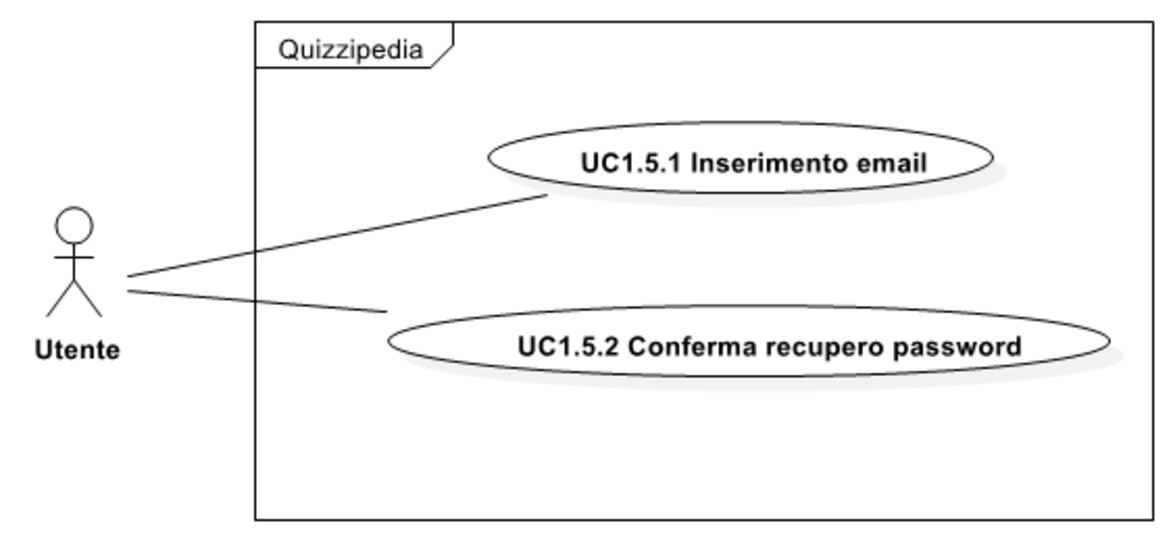
\includegraphics[width=\textwidth]{Img/UC Recupero password.pdf}}
\caption{UC1.5 Recupero password}
\end{figure}
\begin{itemize}
\item \textbf{Attori}: Utente.
\item \textbf{Scenario principale}:
\begin{enumerate}
\item Inserimento email (UC1.5.1);
\item Conferma recupero password (UC1.5.2).
\end{enumerate}
\item \textbf{Estensioni}:
\begin{itemize}
\item Errore in fase di recupero password (UC1.6);
\item Interruzione volontaria del recupero password (UC1.13).
\end{itemize}
\item \textbf{Descrizione}: l’utente in possesso di un account Quizzipedia deve avere la possibilità di accedere al sistema anche in caso di dimenticanza della propria password, a patto che ricordi l’indirizzo email a cui è associato il suo account.
\item \textbf{Precondizione}: l'utente si è connesso al sito web di Quizzipedia attraverso un browser supportato e vuole recuperare l‘accesso al proprio account Quizzipedia.
\item \textbf{Postcondizione}: l’utente ha recuperato l’accesso al proprio account Quizzipedia.
\end{itemize}
\subsubsection{UC1.5.1 Inserimento email}
\begin{itemize}
\item \textbf{Attori}: Utente.
\item \textbf{Scenario principale}: l'utente inserisce il suo indirizzo email.
\item \textbf{Descrizione}: per portare a termine l'operazione, l'utente deve inserire il proprio indirizzo email. Se l'indirizzo email è associato a un account registrato, gli verrà inviata una password temporanea o un link che consentirà all'utente di scegliere una nuova password senza dover ricordare la vecchia.
\item \textbf{Precondizione}: l'utente si trova nella pagina di recupero password e deve ancora inserire l'indirizzo email.
\item \textbf{Postcondizione}: l'utente ha inserito il proprio indirizzo email.
\end{itemize}
\subsubsection{UC1.5.2 Conferma recupero password}
\begin{itemize}
\item \textbf{Attori}: Utente.
\item \textbf{Scenario principale}: l'utente conferma il recupero della password.
\item \textbf{Descrizione}: per portare a termine il recupero password, l'utente deve confermare l'operazione con l'indirizzo email immesso.
\item \textbf{Precondizione}: l'utente si trova in una pagina del sito web che gli permette di confermare il recupero password.
\item \textbf{Postcondizione}: l'utente ha scelto di continuare il recupero password con l'indirizzo email immesso.
\end{itemize}
\subsubsection{UC1.6 Errore in fase di recupero password}
\begin{itemize}
\item \textbf{Attori}: Utente.
\item \textbf{Scenario principale}: l'utente visualizza il messaggio di errore.
\item \textbf{Descrizione}: l'utente visualizza un messaggio di errore che lo avvisa che il tentativo di recupero password non è andato a buon termine.
\item \textbf{Precondizione}: si è verificata la seguente condizione: l'indirizzo email inserito non è associato a un account registrato.
\item \textbf{Postcondizione}: l'utente ha visualizzato il messaggio di errore.
\end{itemize}
\subsubsection{UC1.7 Svolgimento quiz}
\begin{figure}[H]
\centering
\noindent\makebox[\textwidth]{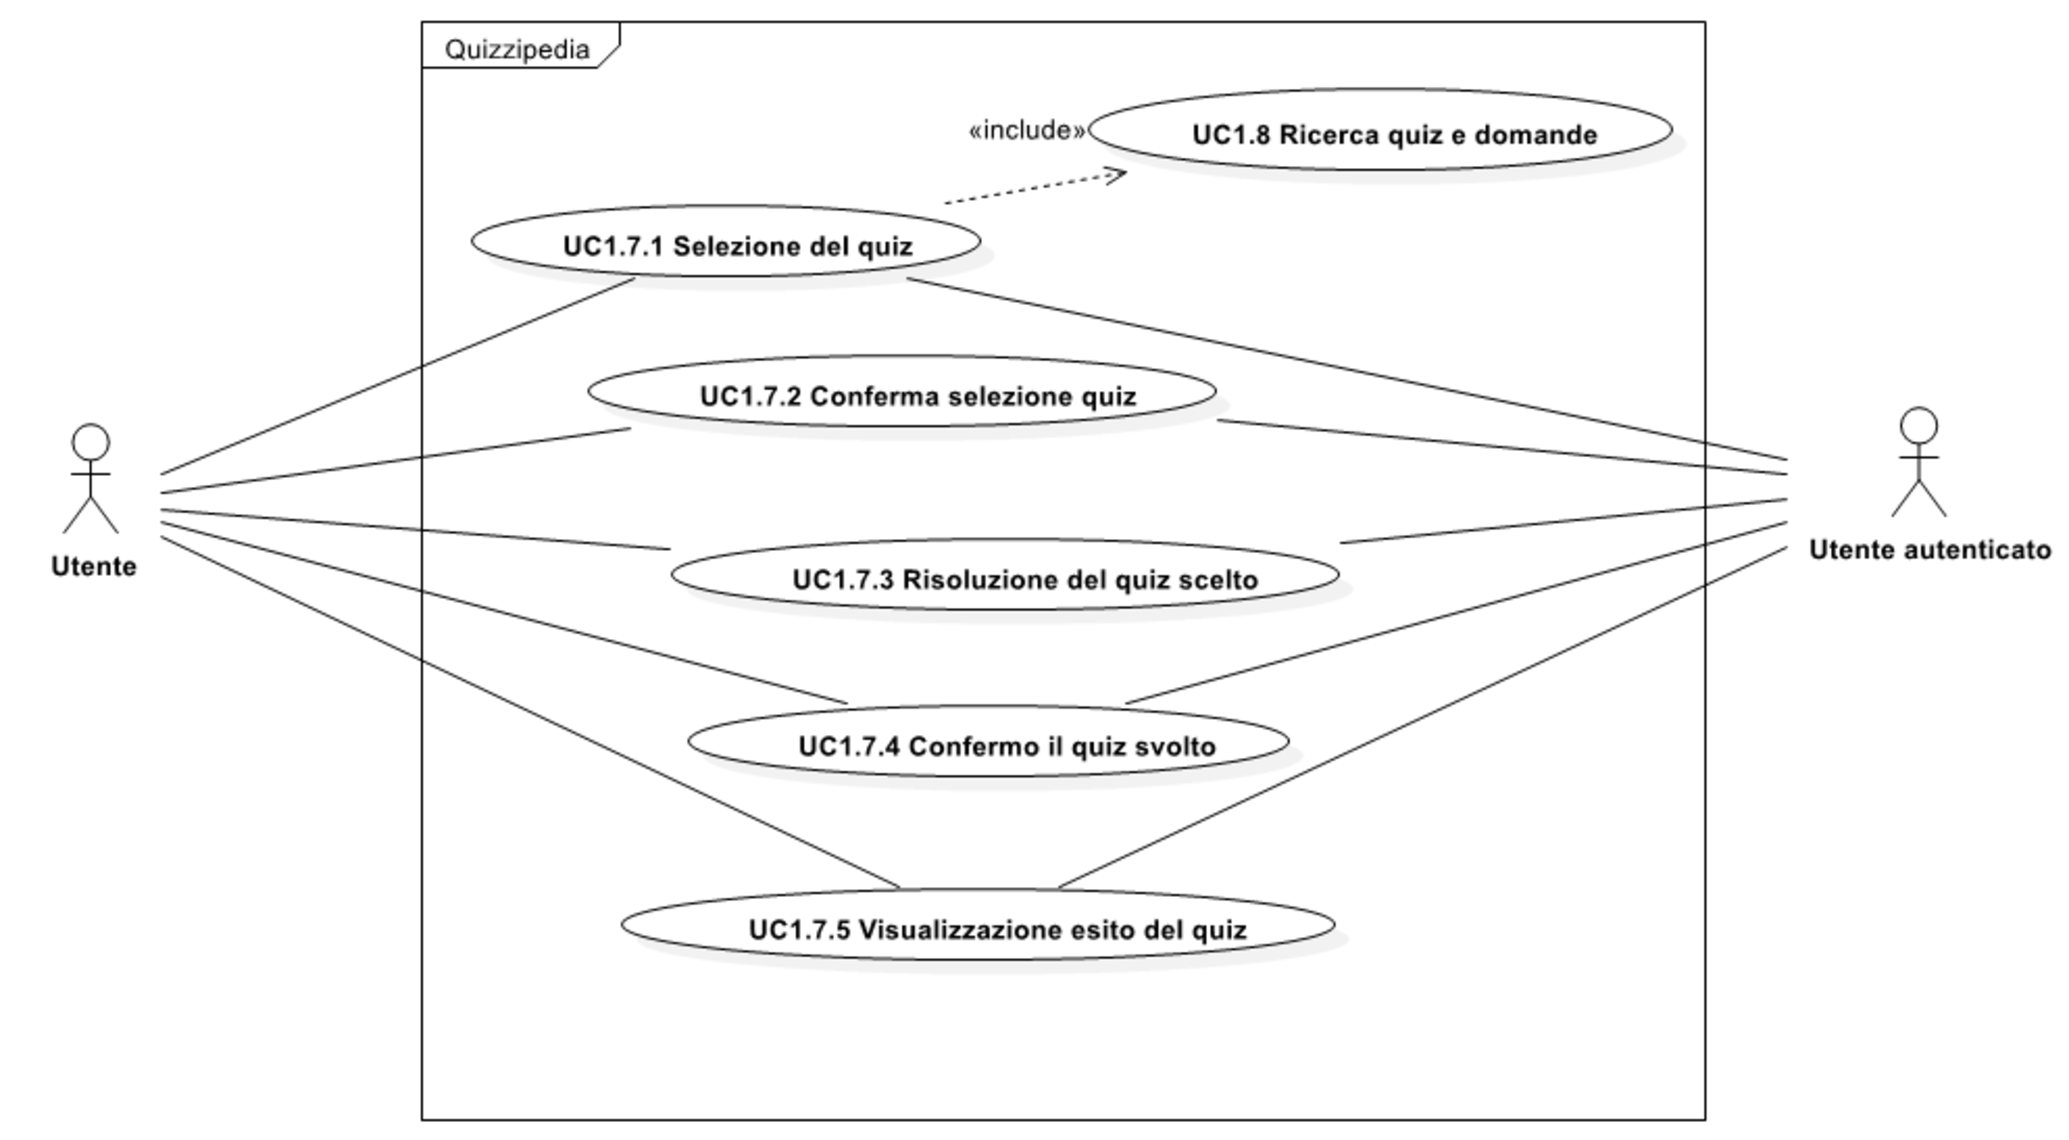
\includegraphics[width=\textwidth]{Img/UC Svolgimento quiz.pdf}}
\caption{UC1.7 Svolgimento quiz}
\end{figure}
\begin{itemize}
\item \textbf{Attori}: Utente, Utente Autenticato.
\item \textbf{Scenario principale}:
\begin{enumerate}
\item Selezione quiz (UC1.7.1);
\item Conferma selezione quiz (UC1.7.2);
\item Risoluzione quiz scelto (UC1.7.3);
\item Conferma risoluzione quiz (UC1.7.4);
\item Visualizzazione esito del quiz (UC1.7.5).
\end{enumerate}
\item \textbf{Estensioni}:
\begin{itemize}
\item Interruzione volontaria dello svolgimento del quiz (UC1.11).
\end{itemize}
\item \textbf{Descrizione}: l'utente deve poter svolgere un quiz conforme ai permessi dell'utente.
\item \textbf{Precondizione}: l'utente sta utilizzando il sistema.
\item \textbf{Postcondizione}: l'utente ha finito di svolgere un quiz.
\end{itemize}
\subsubsection{UC1.7.1 Selezione quiz}
\begin{itemize}
\item \textbf{Attori}: Utente, Utente Autenticato.
\item \textbf{Scenario principale}: l'utente seleziona il quiz da svolgere.
\item \textbf{Descrizione}: l'utente deve poter selezionare il quiz che intende svolgere.
\item \textbf{Precondizione}: l'utente ha scelto di svolgere un quiz e vuole selezionarne uno.
\item \textbf{Postcondizione}: l'utente ha selezionato il quiz.
\end{itemize}
\subsubsection{UC1.7.2 Conferma selezione quiz}
\begin{itemize}
\item \textbf{Attori}: Utente, Utente Autenticato.
\item \textbf{Scenario principale}: l'utente conferma la selezione del quiz.
\item \textbf{Descrizione}: l'utente deve confermare la selezione del quiz scelto per iniziarne lo svolgimento.
\item \textbf{Precondizione}: l'utente ha selezionato il quiz da svolgere e deve confermarlo.
\item \textbf{Postcondizione}: l'utente ha confermato la selezione del quiz.
\end{itemize}
\subsubsection{UC1.7.3 Risoluzione quiz scelto}
\begin{itemize}
\item \textbf{Attori}: Utente, Utente Autenticato.
\item \textbf{Scenario principale}: l'utente risolve il quiz scelto.
\item \textbf{Descrizione}: l'utente deve poter svolgere il quiz che ha selezionato, una domanda alla volta. È possibile spostarsi a piacimento fra le domande e rispondere a una domanda più volte, l'ultima risposta sovrascrive le precedenti.
\item \textbf{Precondizione}: l'utente ha selezionato e confermato un quiz da svolgere.
\item \textbf{Postcondizione}: l'utente ha concluso la risoluzione del quiz.
\end{itemize}
\subsubsection{UC1.7.4 Conferma risoluzione quiz}
\begin{itemize}
\item \textbf{Attori}: Utente, Utente Autenticato.
\item \textbf{Scenario principale}: l'utente conferma la risoluzione del quiz.
\item \textbf{Descrizione}: l'utente deve poter confermare la risoluzione del quiz, terminandone così lo svolgimento. Una volta confermata la risoluzione non sarà più possibile modificare le risposte.
\item \textbf{Precondizione}:  l'utente ha terminato la risoluzione del quiz e vuole riceverne l'esito.
\item \textbf{Postcondizione}: l'utente ha confermato la risoluzione del quiz con le risposte date.
\end{itemize}
\subsubsection{UC1.7.5 Visualizzazione esito del quiz}
\begin{itemize}
\item \textbf{Attori}: Utente, Utente Autenticato.
\item \textbf{Scenario principale}: l'utente visualizza l'esito del quiz svolto.
\item \textbf{Descrizione}: l'utente deve poter visualizzare l'esito del quiz svolto. L'esito può comprendere: il voto ricevuto, la soluzione corretta delle domande a cui è stata data una risposta errata.
\item \textbf{Precondizione}: l'utente ha confermato la risoluzione del quiz svolto.
\item \textbf{Postcondizione}: l'utente ha visualizzato l'esito.
\end{itemize}
\subsubsection{UC1.8 Ricerca quiz e domande}
\begin{figure}[H]
\centering
\noindent\makebox[\textwidth]{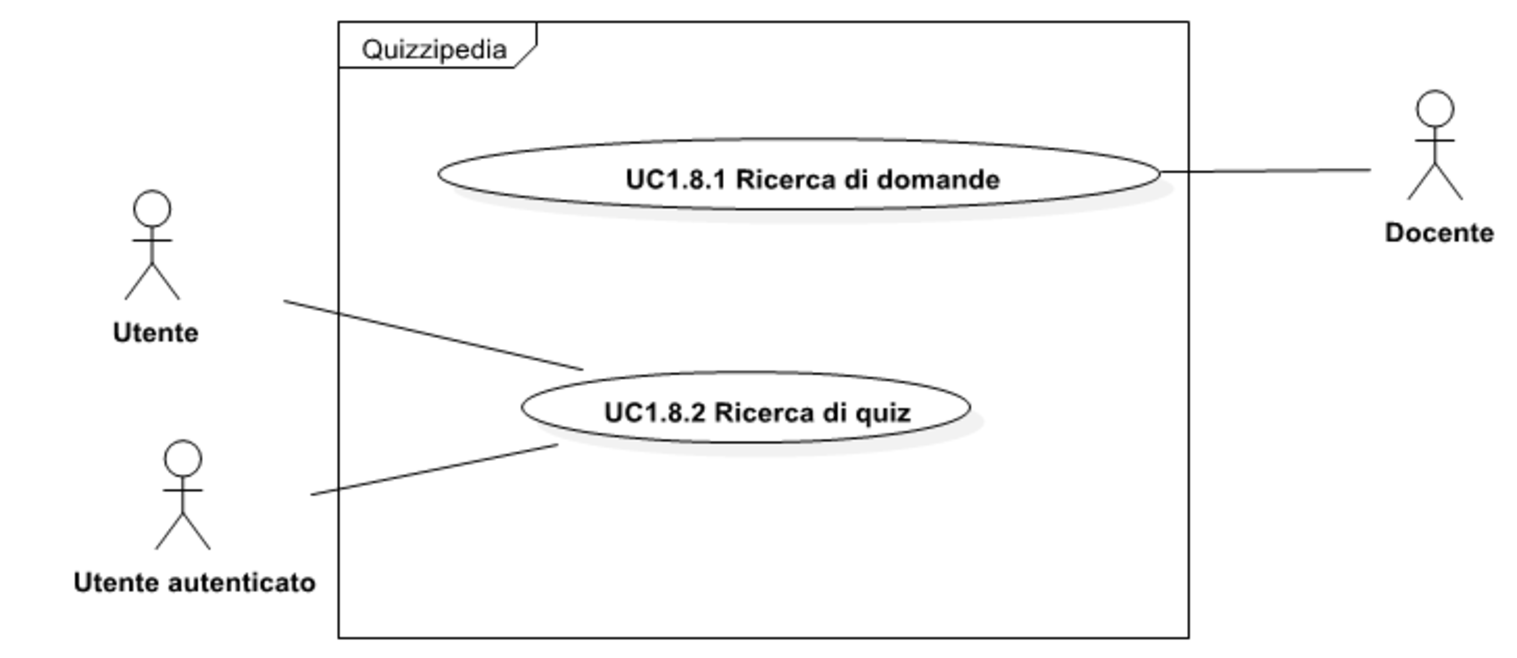
\includegraphics[width=\textwidth]{Img/UC Ricerca quiz e domande.pdf}}
\caption{UC1.8 Ricerca quiz e domande}
\end{figure}
\begin{itemize}
\item \textbf{Attori}: Docente, Utente, Utente Autenticato.
\item \textbf{Scenario principale}:
\begin{enumerate}
\item Ricerca di domande (UC1.8.1);
\item Ricerca di quiz (UC1.8.2).
\end{enumerate}
\item \textbf{Estensioni}:
\begin{itemize}
\item Interruzione volontaria della ricerca (UC1.12).
\end{itemize}
\item \textbf{Descrizione}: il docente e i vari tipi di utente possono effettuare una ricerca di quiz e domande presenti nel sistema. La ricerca è personalizzabile attraverso vari parametri di ricerca.
\item \textbf{Precondizione}: il docente e gli altri utenti registrati sono autenticati nel sistema, l'utente 'guest' non è autenticato.
\item \textbf{Postcondizione}: il docente e i vari tipi di utente hanno effettuato la ricerca.
\end{itemize}
\subsubsection{UC1.8.1 Ricerca di domande}
\begin{figure}[H]
\centering
\noindent\makebox[\textwidth]{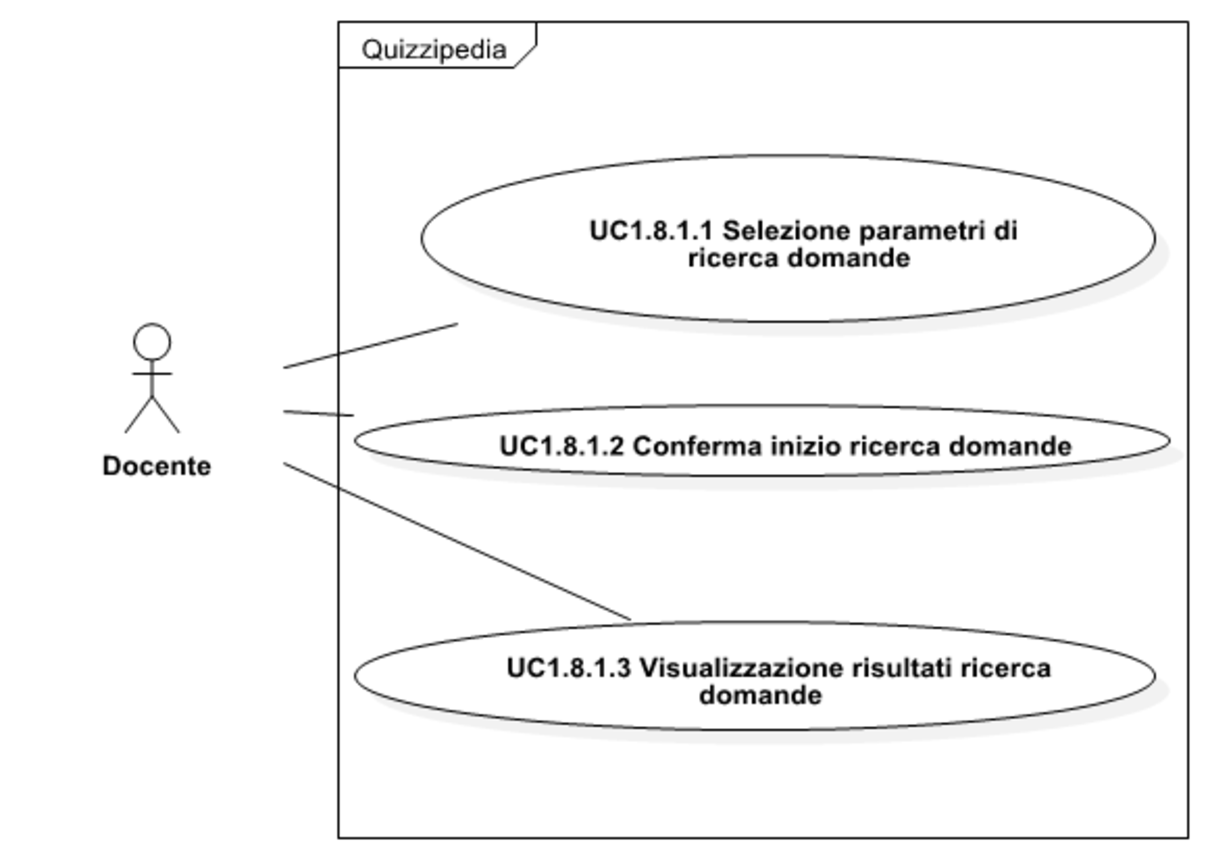
\includegraphics[width=\textwidth]{Img/UC Ricerca di domande.pdf}}
\caption{UC1.8.1 Ricerca di domande}
\end{figure}
\begin{itemize}
\item \textbf{Attori}: Docente.
\item \textbf{Scenario principale}:
\begin{enumerate}
\item Selezione parametri di ricerca domande (UC1.8.1.1);
\item Conferma inizio ricerca domande (UC1.8.1.2);
\item Visualizzazione risultati ricerca domande (UC1.8.1.3).
\end{enumerate}
\item \textbf{Scenario principale}: il docente cerca delle domande.
\item \textbf{Descrizione}: il docente deve poter cercare domande.
\item \textbf{Precondizione}: il docente sta effettuando una ricerca.
\item \textbf{Postcondizione}: il docente ha effettuato la ricerca di domande.
\end{itemize}
\subsubsection{UC1.8.1.1 Selezione parametri di ricerca domande}
\begin{figure}[H]
\centering
\noindent\makebox[\textwidth]{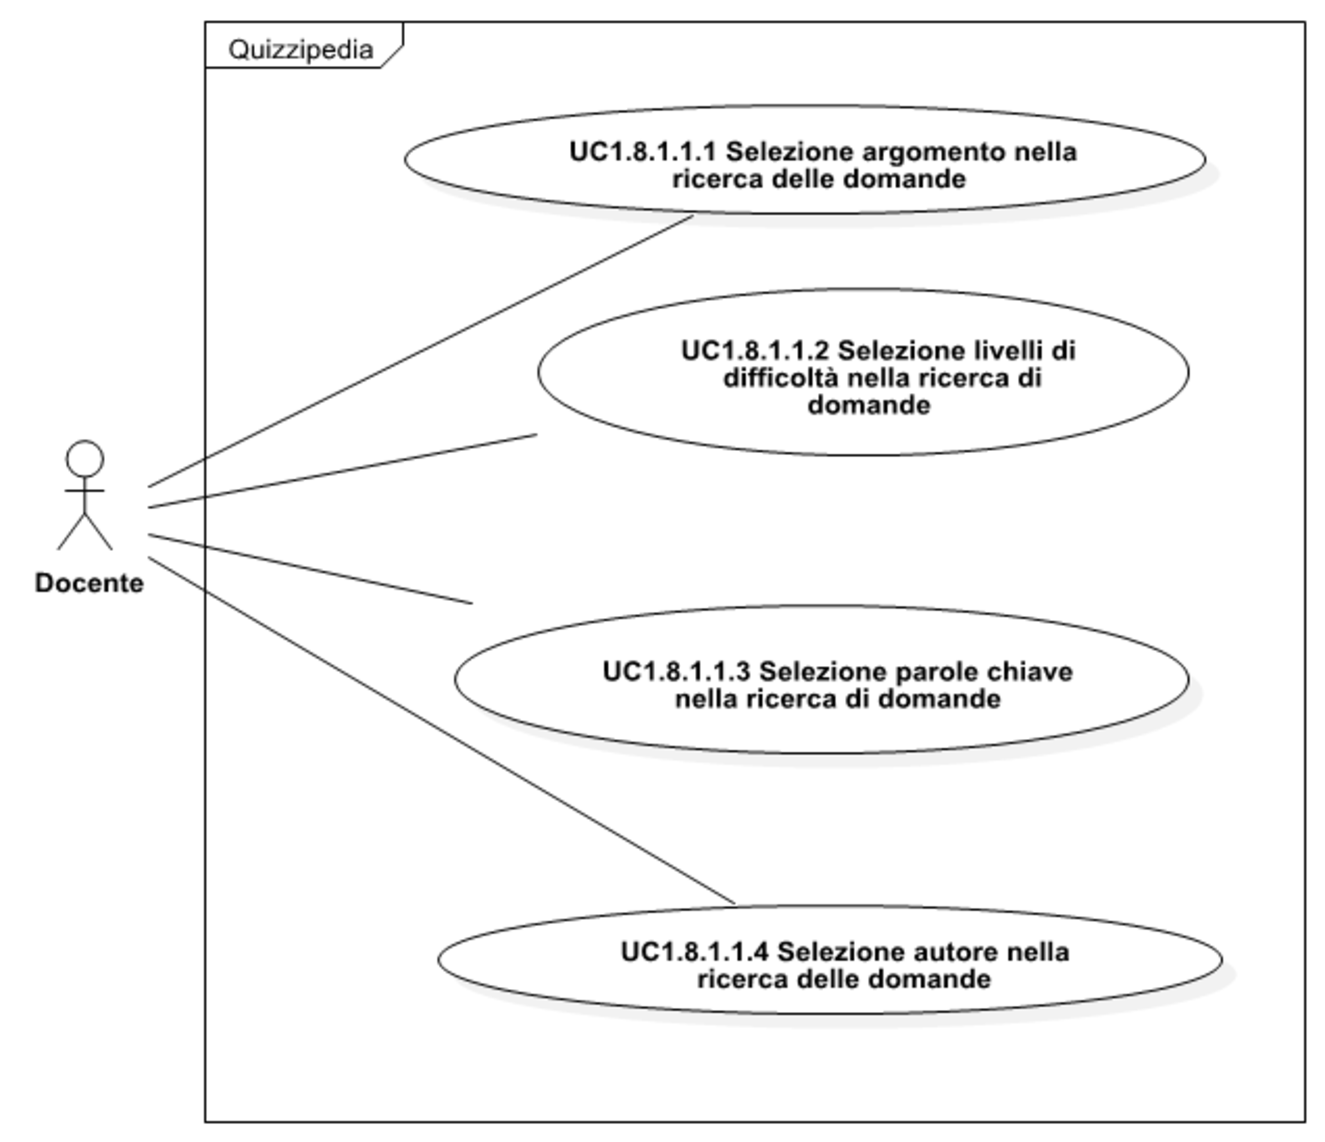
\includegraphics[width=\textwidth]{Img/UC Selezione parametri di ricerca domande.pdf}}
\caption{UC1.8.1.1 Selezione parametri di ricerca domande}
\end{figure}
\begin{itemize}
\item \textbf{Attori}: Docente.
\item \textbf{Scenario principale}:
\begin{enumerate}
\item Selezione argomenti nella ricerca delle domande (UC1.8.1.1.1);
\item Selezione livelli di difficoltà nella ricerca delle domande (UC1.8.1.1.2);
\item Selezione parole chiave nella ricerca di domande (UC1.8.1.1.3);
\item Selezione autore nella ricerca di domande (UC1.8.1.1.4).
\end{enumerate}
\item \textbf{Descrizione}: il docente deve poter personalizzare la ricerca di domande attraverso diversi parametri.
\item \textbf{Precondizione}: il docente ha scelto di effettuare una ricerca di domande.
\item \textbf{Postcondizione}: il docente ha selezionato i parametri desiderati nella ricerca di domande.
\end{itemize}
\subsubsection{UC1.8.1.1.1 Selezione argomenti nella ricerca delle domande}
\begin{itemize}
\item \textbf{Attori}: Docente.
\item \textbf{Scenario principale}: il docente seleziona/deseleziona gli argomenti delle domande.
\item \textbf{Descrizione}: il docente deve poter selezionare/deselezionare uno o più argomenti, escludendo domande di argomenti non selezionati dalla ricerca.
\item \textbf{Precondizione}: il docente sta personalizzando la ricerca di domande attraverso dei parametri.
\item \textbf{Postcondizione}: il docente ha selezionato/deselezionato gli argomenti delle domande.
\end{itemize}
\subsubsection{UC1.8.1.1.2 Selezione livelli di difficoltà nella ricerca delle domande}
\begin{itemize}
\item \textbf{Attori}: Docente.
\item \textbf{Scenario principale}: il docente seleziona/deseleziona i livelli di difficoltà delle domande.
\item \textbf{Descrizione}: il docente deve poter selezionare/deselezionare uno o più livelli di difficoltà, escludendo domande di livello di difficoltà non selezionato.
\item \textbf{Precondizione}: il docente sta personalizzando la ricerca di domande attraverso dei parametri.
\item \textbf{Postcondizione}: il docente ha selezionato/deselezionato i livelli di difficoltà delle domande.
\end{itemize}
\subsubsection{UC1.8.1.1.3 Selezione parole chiave nella ricerca di domande}
\begin{itemize}
\item \textbf{Attori}: Docente.
\item \textbf{Scenario principale}: il docente seleziona/deseleziona le parole chiave delle domande.
\item \textbf{Descrizione}: il docente deve poter selezionare/deselezionare una o più parole chiave, escludendo le domande in cui le parole chiave immesse non compaiono nel titolo o nella descrizione.
\item \textbf{Precondizione}: il docente sta personalizzando la ricerca delle domande attraverso dei parametri.
\item \textbf{Postcondizione}: il docente ha selezionato/deselezionato le parole chiave delle domande.
\end{itemize}
\subsubsection{UC1.8.1.1.4 Selezione autore nella ricerca di domande}
\begin{itemize}
\item \textbf{Attori}: Docente.
\item \textbf{Scenario principale}: il docente inserisce il nome dell'autore delle domande che vuole trovare.
\item \textbf{Descrizione}: il docente deve poter cercare le domande attraverso il nome del loro autore.
\item \textbf{Precondizione}: il docente sta personalizzando la ricerca delle domande attraverso dei parametri.
\item \textbf{Postcondizione}: il docente ha inserito il nome dell'autore delle domande che vuole cercare.
\end{itemize}
\subsubsection{UC1.8.1.2 Conferma inizio ricerca domande}
\begin{itemize}
\item \textbf{Attori}: Docente.
\item \textbf{Scenario principale}: il docente conferma l'inizio della ricerca di domande.
\item \textbf{Descrizione}: il docente deve poter confermare l'inizio della ricerca di domande. Se sono stati inseriti dei parametri, questi dovranno essere tenuti in considerazione.
\item \textbf{Precondizione}: il docente ha scelto di effettuare una ricerca di domande e selezionato eventuali parametri.
\item \textbf{Postcondizione}: il docente ha confermato l'inizio della ricerca delle domande.
\end{itemize}
\subsubsection{UC1.8.1.3 Visualizzazione risultati ricerca domande}
\begin{itemize}
\item \textbf{Attori}: Docente.
\item \textbf{Scenario principale}: il docente visualizza la lista dei risultati prodotti dalla ricerca di domande.
\item \textbf{Descrizione}: il docente deve poter visualizzare la lista dei risultati prodotti dalla ricerca di domande effettuata.
\item \textbf{Precondizione}: il docente ha scelto di effettuare una ricerca di domande, selezionato eventuali parametri e confermato l'avvio della ricerca.
\item \textbf{Postcondizione}: il docente ha visualizzato i risultati prodotti dalla ricerca di domande effettuata.
\end{itemize}
\subsubsection{UC1.8.2 Ricerca di quiz}
\begin{figure}[H]
\centering
\noindent\makebox[\textwidth]{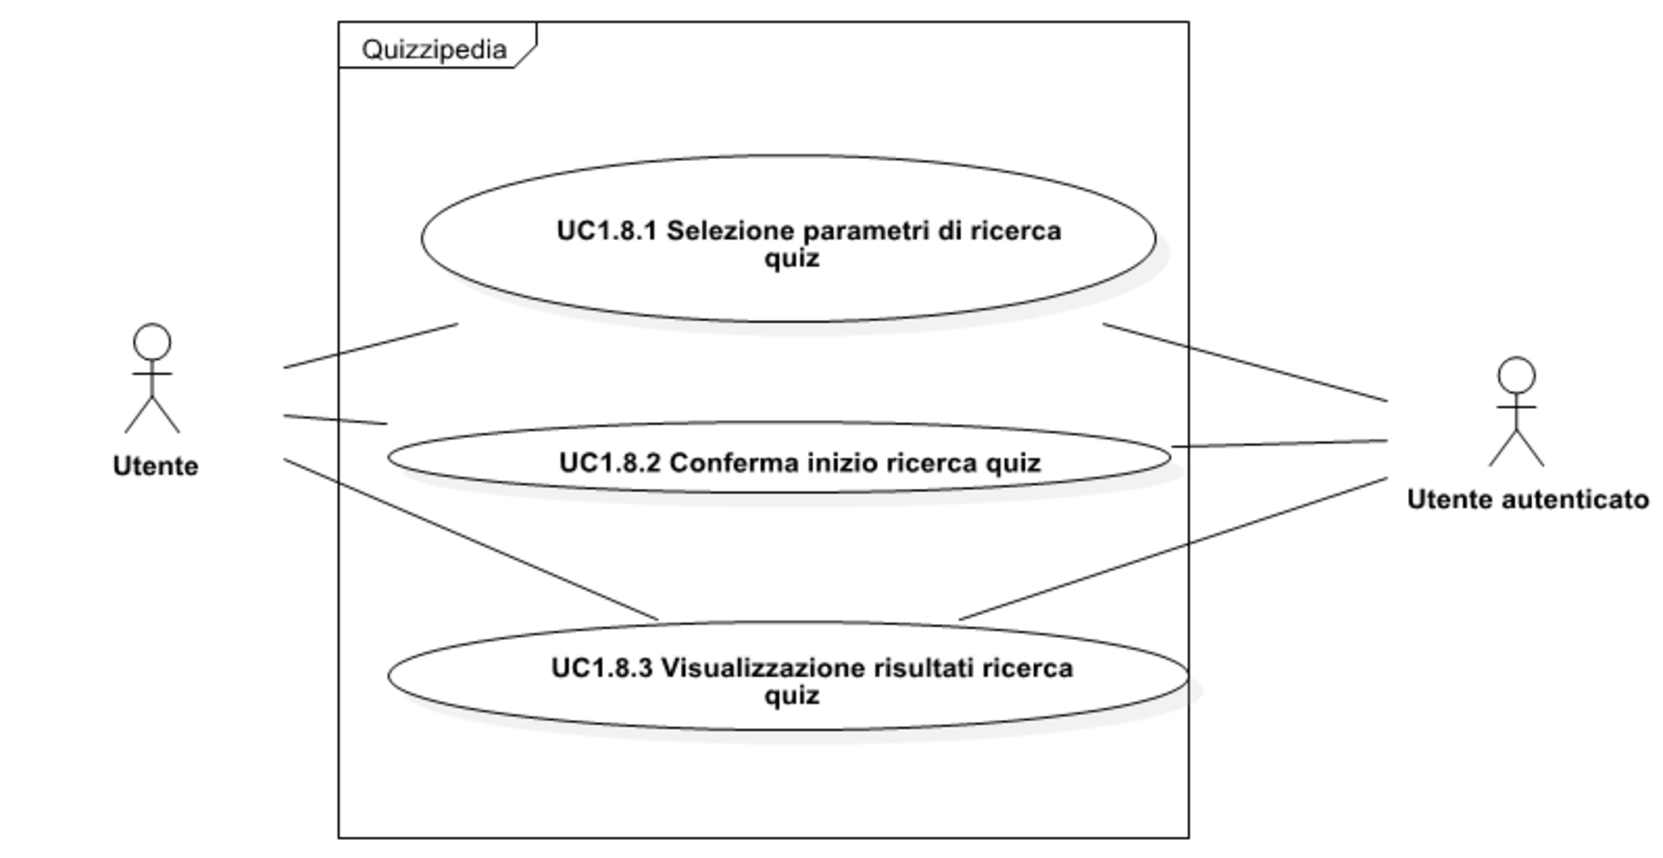
\includegraphics[width=\textwidth]{Img/UC Ricerca di quiz.pdf}}
\caption{UC1.8.2 Ricerca di quiz}
\end{figure}
\begin{itemize}
\item \textbf{Attori}: Utente, Utente Autenticato.
\item \textbf{Scenario principale}:
\begin{enumerate}
\item Selezione parametri di ricerca quiz (UC1.8.2.1);
\item Conferma inizio ricerca quiz (UC1.8.2.2);
\item Visualizzazione risultati ricerca quiz (UC1.8.2.3).
\end{enumerate}
\item \textbf{Descrizione}: l'utente deve poter cercare dei quiz.
\item \textbf{Precondizione}: l'utente sta effettuando una ricerca.
\item \textbf{Postcondizione}: l'utente ha effettuato la ricerca di quiz.
\end{itemize}
\subsubsection{UC1.8.2.1 Selezione parametri di ricerca quiz}
\begin{figure}[H]
\centering
\noindent\makebox[\textwidth]{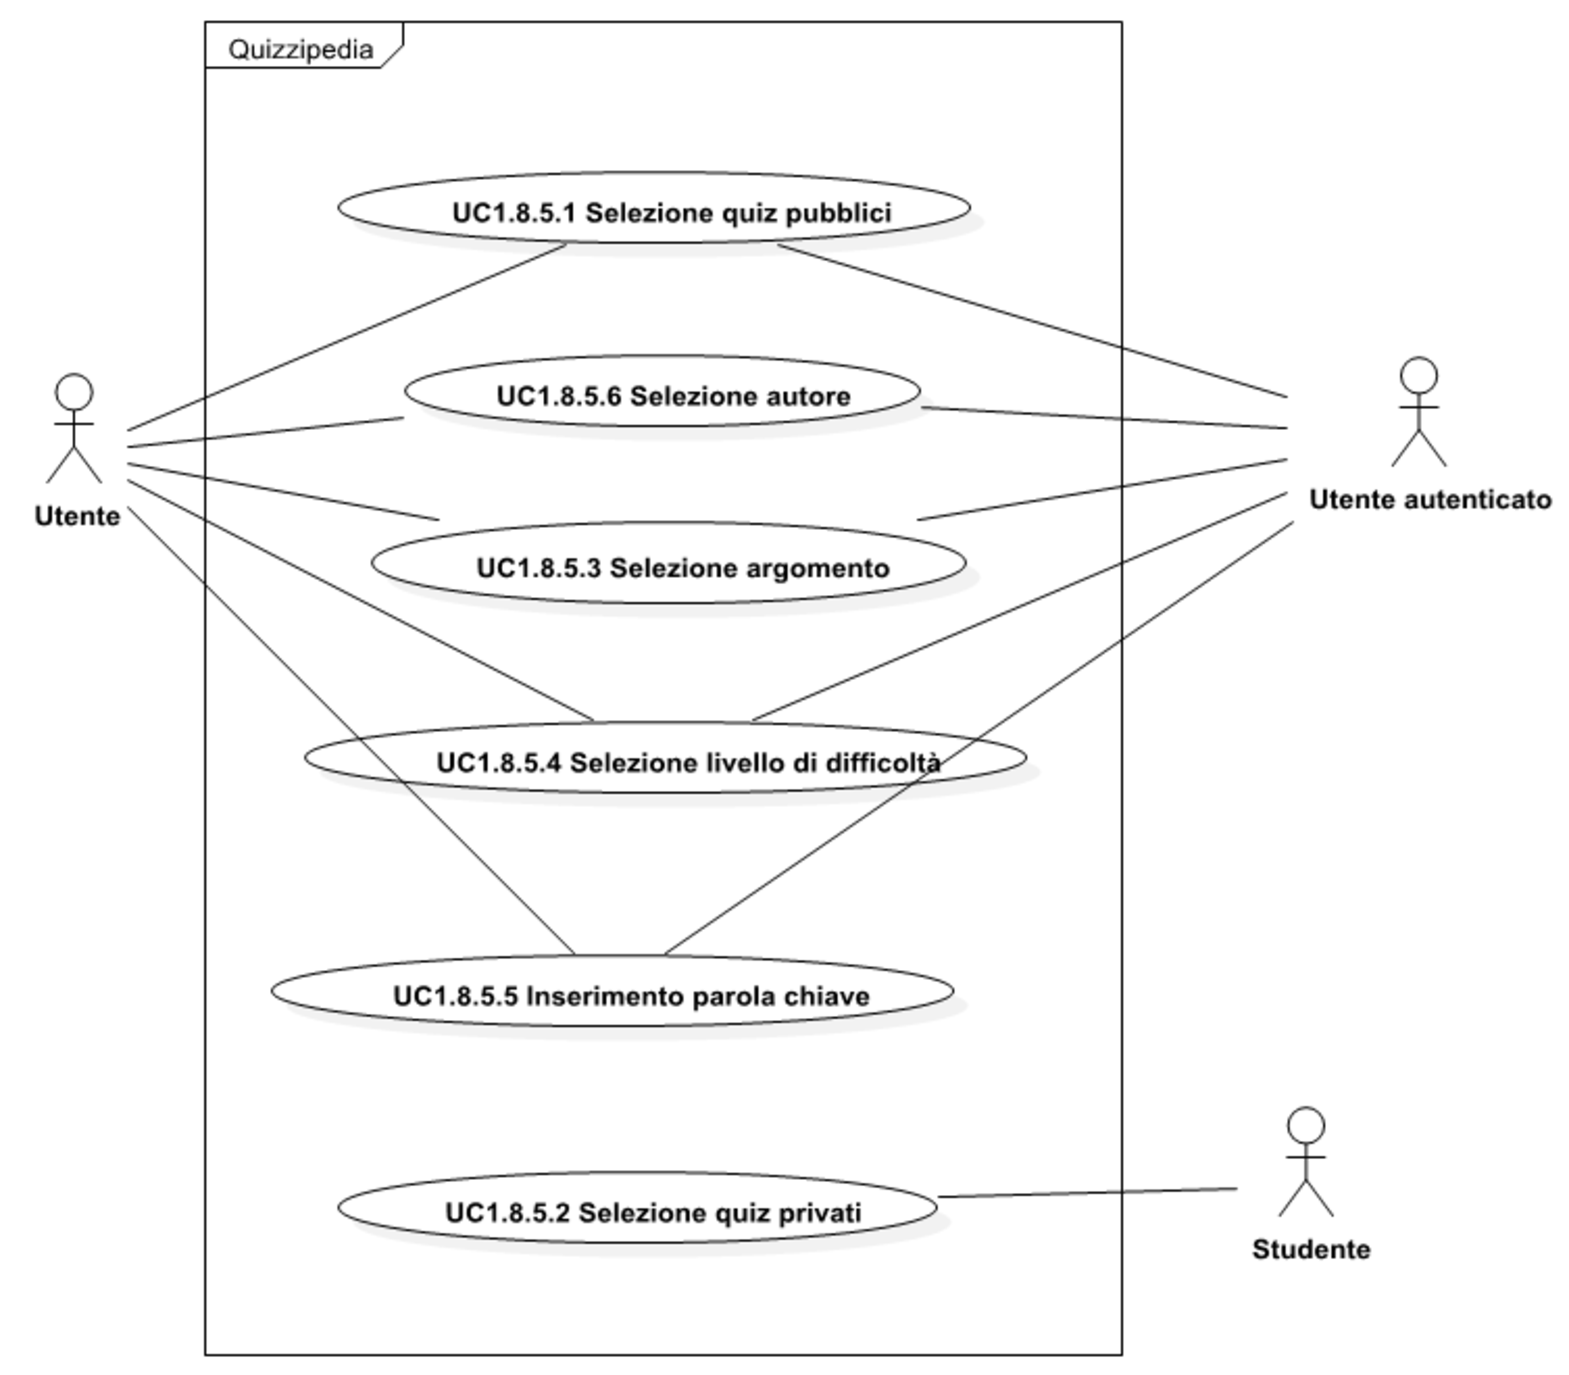
\includegraphics[width=\textwidth]{Img/UC Selezione parametri di ricerca quiz.pdf}}
\caption{UC1.8.2.1 Selezione parametri di ricerca quiz}
\end{figure}
\begin{itemize}
\item \textbf{Attori}: Studente, Utente, Utente Autenticato.
\item \textbf{Scenario principale}:
\begin{enumerate}
\item Selezione quiz pubblici (UC1.8.2.1.1);
\item Selezione quiz privati (UC1.8.2.1.2);
\item Selezione argomenti nella ricerca di quiz (UC1.8.2.1.3);
\item Selezione livelli di difficoltà nella ricerca di quiz (UC1.8.2.1.4);
\item Selezione parole chiave nella ricerca di quiz (UC1.8.2.1.5);
\item Selezione autore nella ricerca di quiz (UC1.8.2.1.6).
\end{enumerate}
\item \textbf{Descrizione}: l'utente deve poter personalizzare la ricerca di quiz attraverso diversi parametri.
\item \textbf{Precondizione}: l'utente ha scelto di effettuare una ricerca di quiz.
\item \textbf{Postcondizione}: l'utente ha selezionato i parametri desiderati nella ricerca di quiz.
\end{itemize}
\subsubsection{UC1.8.2.1.1 Selezione quiz pubblici}
\begin{itemize}
\item \textbf{Attori}: Utente, Utente Autenticato.
\item \textbf{Scenario principale}: l'utente seleziona/deseleziona l'opzione 'quiz pubblico'.
\item \textbf{Descrizione}: l'utente deve poter selezionare/deselezionare l'opzione 'quiz pubblico', che escluderà dalla ricerca i quiz privati.
\item \textbf{Precondizione}: l'utente sta personalizzando la ricerca attraverso dei parametri.
\item \textbf{Postcondizione}: l'utente ha selezionato/deselezionato il parametro 'quiz pubblico'.
\end{itemize}
\subsubsection{UC1.8.2.1.2 Selezione quiz privati}
\begin{figure}[H]
\centering
\noindent\makebox[\textwidth]{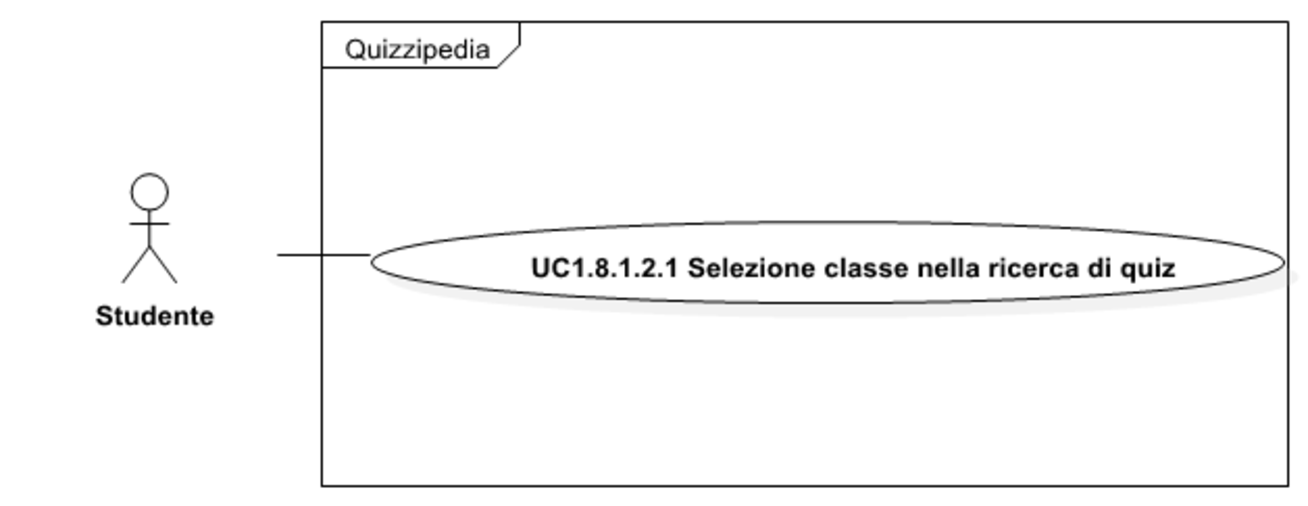
\includegraphics[width=\textwidth]{Img/UC Selezione quiz privati.pdf}}
\caption{UC1.8.2.1.2 Selezione quiz privati}
\end{figure}
\begin{itemize}
\item \textbf{Attori}: Studente.
\item \textbf{Scenario principale}:
\begin{enumerate}
\item Selezione classe nella ricerca di quiz (UC1.8.2.1.2.1).
\end{enumerate}
\item \textbf{Scenario principale}: lo studente seleziona/deseleziona l'opzione 'quiz privato'.
\item \textbf{Descrizione}: lo studente deve poter selezionare/deselezionare l'opzione 'quiz privato', che escluderà dalla ricerca i quiz pubblici.
\item \textbf{Precondizione}: lo studente  sta personalizzando la ricerca attraverso dei parametri.
\item \textbf{Postcondizione}: lo studente  ha selezionato/deselezionato il parametro 'quiz privato'.
\end{itemize}
\subsubsection{UC1.8.2.1.2.1 Selezione classe nella ricerca di quiz}
\begin{itemize}
\item \textbf{Attori}: Studente.
\item \textbf{Descrizione}: lo studente deve poter selezionare/deselezionare una classe a cui appartiene per visualizzarne i quiz disponibili.
\item \textbf{Precondizione}: lo studente ha selezionato 'quiz privati' come parametro della sua ricerca.
\item \textbf{Postcondizione}: lo studente ha selezionato/deselezionato la classe come parametro della sua ricerca di quiz.
\end{itemize}
\subsubsection{UC1.8.2.1.3 Selezione argomenti nella ricerca di quiz}
\begin{itemize}
\item \textbf{Attori}: Utente, Utente Autenticato.
\item \textbf{Scenario principale}: l'utente seleziona/deseleziona gli argomenti dei quiz.
\item \textbf{Descrizione}: l'utente deve poter selezionare/deselezionare uno o più argomenti, escludento quiz di argomenti non selezionati dalla ricerca.
\item \textbf{Precondizione}: l'utente sta effettuando una ricerca si quiz.
\item \textbf{Postcondizione}: l'utente ha selezionato/deselezionato gli argomenti dei quiz.
\end{itemize}
\subsubsection{UC1.8.2.1.4 Selezione livelli di difficoltà nella ricerca di quiz}
\begin{itemize}
\item \textbf{Attori}: Utente, Utente Autenticato.
\item \textbf{Scenario principale}: l'utente seleziona/deseleziona i livelli di difficoltà dei quiz.
\item \textbf{Descrizione}: l'utente deve poter selezionare/deselezionare uno o più livelli di difficoltà, escludento quiz di argomenti non selezionati dalla ricerca.
\item \textbf{Precondizione}: l'utente sta personalizzando la ricerca di quiz attraverso dei parametri.
\item \textbf{Postcondizione}: l'utente ha selezionato/deselezionato i livelli di difficoltà dei quiz.
\end{itemize}
\subsubsection{UC1.8.2.1.5 Selezione parole chiave nella ricerca di quiz}
\begin{itemize}
\item \textbf{Attori}: Utente, Utente Autenticato.
\item \textbf{Scenario principale}: l'utente seleziona/deseleziona le parole chiave dei quiz.
\item \textbf{Descrizione}: l'utente deve poter selezionare/deselezionare una o più parole chiave, escludento quiz di argomenti non selezionati dalla ricerca.
\item \textbf{Precondizione}: l'utente sta personalizzando la ricerca dei quiz attraverso dei parametri.
\item \textbf{Postcondizione}: l'utente ha selezionato/deselezionato le parole chiave dei quiz.
\end{itemize}
\subsubsection{UC1.8.2.1.6 Selezione autore nella ricerca di quiz}
\begin{itemize}
\item \textbf{Attori}: Utente, Utente Autenticato.
\item \textbf{Scenario principale}: l'utente seleziona/deseleziona l'autore del quiz.
\item \textbf{Descrizione}: l'utente deve poter selezionare/deselezionare l'autore dei quiz che sta cercando.
\item \textbf{Precondizione}: l'utente sta personalizzando la ricerca dei quiz attraverso dei parametri.
\item \textbf{Postcondizione}: l'utente ha selezionato/deselezionato l'autore dei quiz.
\end{itemize}
\subsubsection{UC1.8.2.2 Conferma inizio ricerca quiz}
\begin{itemize}
\item \textbf{Attori}: Utente, Utente Autenticato.
\item \textbf{Scenario principale}: l'utente conferma l'inizio della ricerca di quiz.
\item \textbf{Descrizione}: l'utente deve poter confermare l'inizio della ricerca di  quiz. Se sono stati inseriti dei parametri, questi dovranno essere tenuti in considerazione.
\item \textbf{Precondizione}: l'utente ha scelto di effettuare una ricerca di quiz e selezionato eventuali parametri.
\item \textbf{Postcondizione}: l'utente ha confermato l'inizio della ricerca dei quiz.
\end{itemize}
\subsubsection{UC1.8.2.3 Visualizzazione risultati ricerca quiz}
\begin{itemize}
\item \textbf{Attori}: Utente, Utente Autenticato.
\item \textbf{Scenario principale}: l'utente visualizza la lista dei risultati prodotti dalla ricerca di quiz.
\item \textbf{Descrizione}: l'utente deve poter visualizzare la lista dei risultati prodotti dalla ricerca di quiz effettuata.
\item \textbf{Precondizione}: l'utente ha scelto di effettuare una ricerca di quiz, selezionato eventuali parametri e confermato l'avvio della ricerca.
\item \textbf{Postcondizione}: l'utente ha visualizzato i risultati prodotti dalla ricerca di quiz effettuata.
\end{itemize}
\subsubsection{UC1.9 Interruzione volontaria della registrazione}
\begin{itemize}
\item \textbf{Attori}: Utente.
\item \textbf{Scenario principale}: l'utente interrompe la ricerca.
\item \textbf{Descrizione}: L'utente può interrompere volontariamente la registrazione.
\item \textbf{Precondizione}: L'utente sta svolgendo la registrazione.
\item \textbf{Postcondizione}: La registrazione non è stata completata.
\end{itemize}
\subsubsection{UC1.10 Interruzione volontaria dell'autenticazione}
\begin{itemize}
\item \textbf{Attori}: Utente.
\item \textbf{Scenario principale}: l'utente interrompe l'autenticazione.
\item \textbf{Descrizione}: l'utente interrompe volontariamente l'autenticazione.
\item \textbf{Precondizione}: L'utente sta svolgendo l'autenticazione.
\item \textbf{Postcondizione}: L'autenticazione non è stata completata.
\end{itemize}
\subsubsection{UC1.11 Interruzione volontaria dello svolgimento del quiz}
\begin{itemize}
\item \textbf{Attori}: Utente, Utente Autenticato.
\item \textbf{Scenario principale}: l'utente interrompe lo svolgimento del quiz.
\item \textbf{Descrizione}: l'utente ha interrotto lo svolgimento del quiz.
\item \textbf{Precondizione}: l'utente sta svolgendo un quiz.
\item \textbf{Postcondizione}: l'utente non ha completato lo svolgimento del quiz.
\end{itemize}
\subsubsection{UC1.12 Interruzione volontaria della ricerca}
\begin{itemize}
\item \textbf{Attori}: Utente, Utente Autenticato.
\item \textbf{Scenario principale}: l'utente interrompe la ricerca.
\item \textbf{Descrizione}: l'utente ha interrotto la ricerca.
\item \textbf{Precondizione}: l'utente sta effettuando una ricerca.
\item \textbf{Postcondizione}: l'utente non ha portato a termine la ricerca.
\end{itemize}
\subsubsection{UC1.13 Interruzione volontaria del recupero password}
\begin{itemize}
\item \textbf{Attori}: Utente.
\item \textbf{Scenario principale}: l'utente interrompe il recupero della password.
\item \textbf{Descrizione}: L'utente interrompe volontariamente il recupero della password.
\item \textbf{Precondizione}: l'utente sta effettuando il recupero della password.
\item \textbf{Postcondizione}: l'utente non ha completato il recupero della password.
\end{itemize}
\subsubsection{UC2 Caso d'uso privato}
\begin{figure}[H]
\centering
\noindent\makebox[\textwidth]{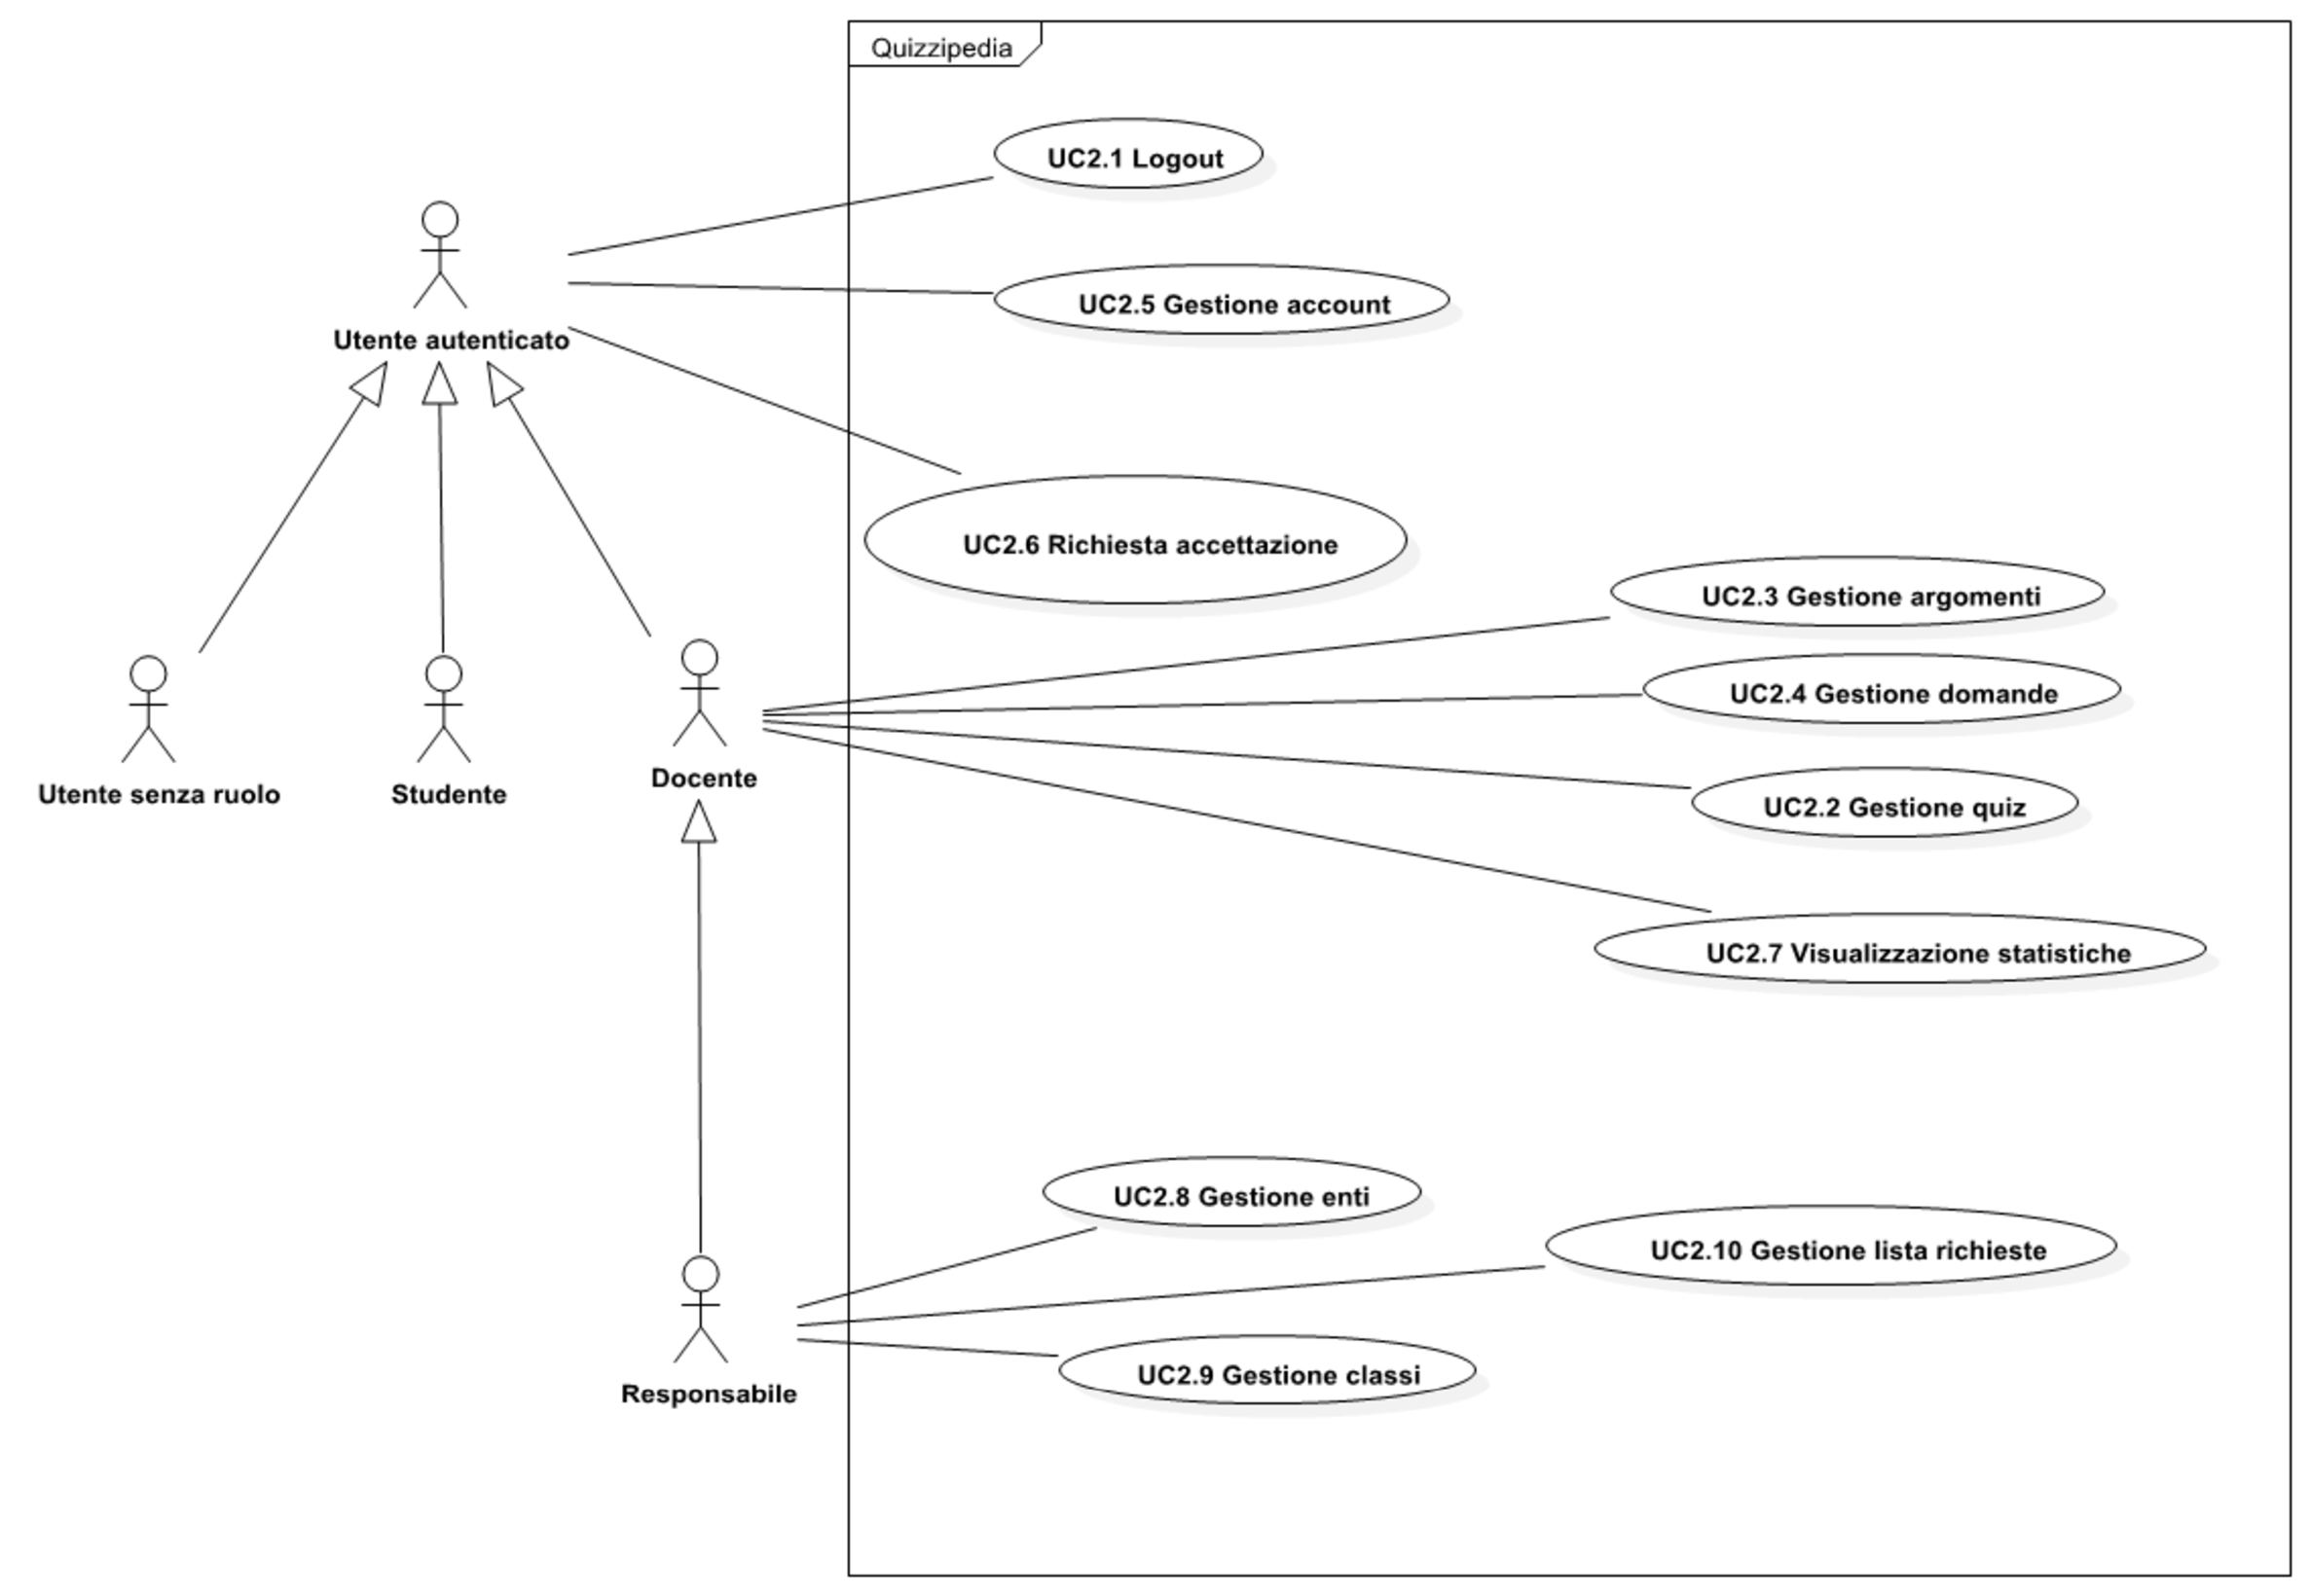
\includegraphics[width=\textwidth]{Img/UC Caso d'uso privato.pdf}}
\caption{UC2 Caso d'uso privato}
\end{figure}
\begin{itemize}
\item \textbf{Attori}: Utente Autenticato.
\item \textbf{Scenario principale}:
\begin{enumerate}
\item Logout (UC2.1);
\item Gestione quiz (UC2.2);
\item Gestione argomenti (UC2.3);
\item Gestione account (UC2.4);
\item Richiesta accettazione (UC2.5);
\item Visualizzazione statistiche (UC2.6);
\item Modifica ente (UC2.7);
\item Gestione classi (UC2.8);
\item Gestione richieste (UC2.9);
\item Gestione domande (UC2.10).
\end{enumerate}
\item \textbf{Descrizione}: l'utente autenticato può accedere ad aree private a seconda dei permessi di cui dispone.
\item \textbf{Precondizione}: l'utente è in possesso di un account Quizzipedia e si è precedentemente autenticato.
\item \textbf{Postcondizione}: l'utente ha scelto l'operazione da intraprendere.
\end{itemize}
\subsubsection{UC2.1 Logout}
\begin{itemize}
\item \textbf{Attori}: Utente Autenticato.
\item \textbf{Descrizione}: l’utente può effettuare il logout dall’area privata.
\item \textbf{Precondizione}: l’utente è in possesso di un account Quizzipedia e si è precedentemente autenticato.
\item \textbf{Postcondizione}: l’utente ha effettuato il logout e ora non è più autenticato.
\end{itemize}
\subsubsection{UC2.2 Gestione quiz}
\begin{figure}[H]
\centering
\noindent\makebox[\textwidth]{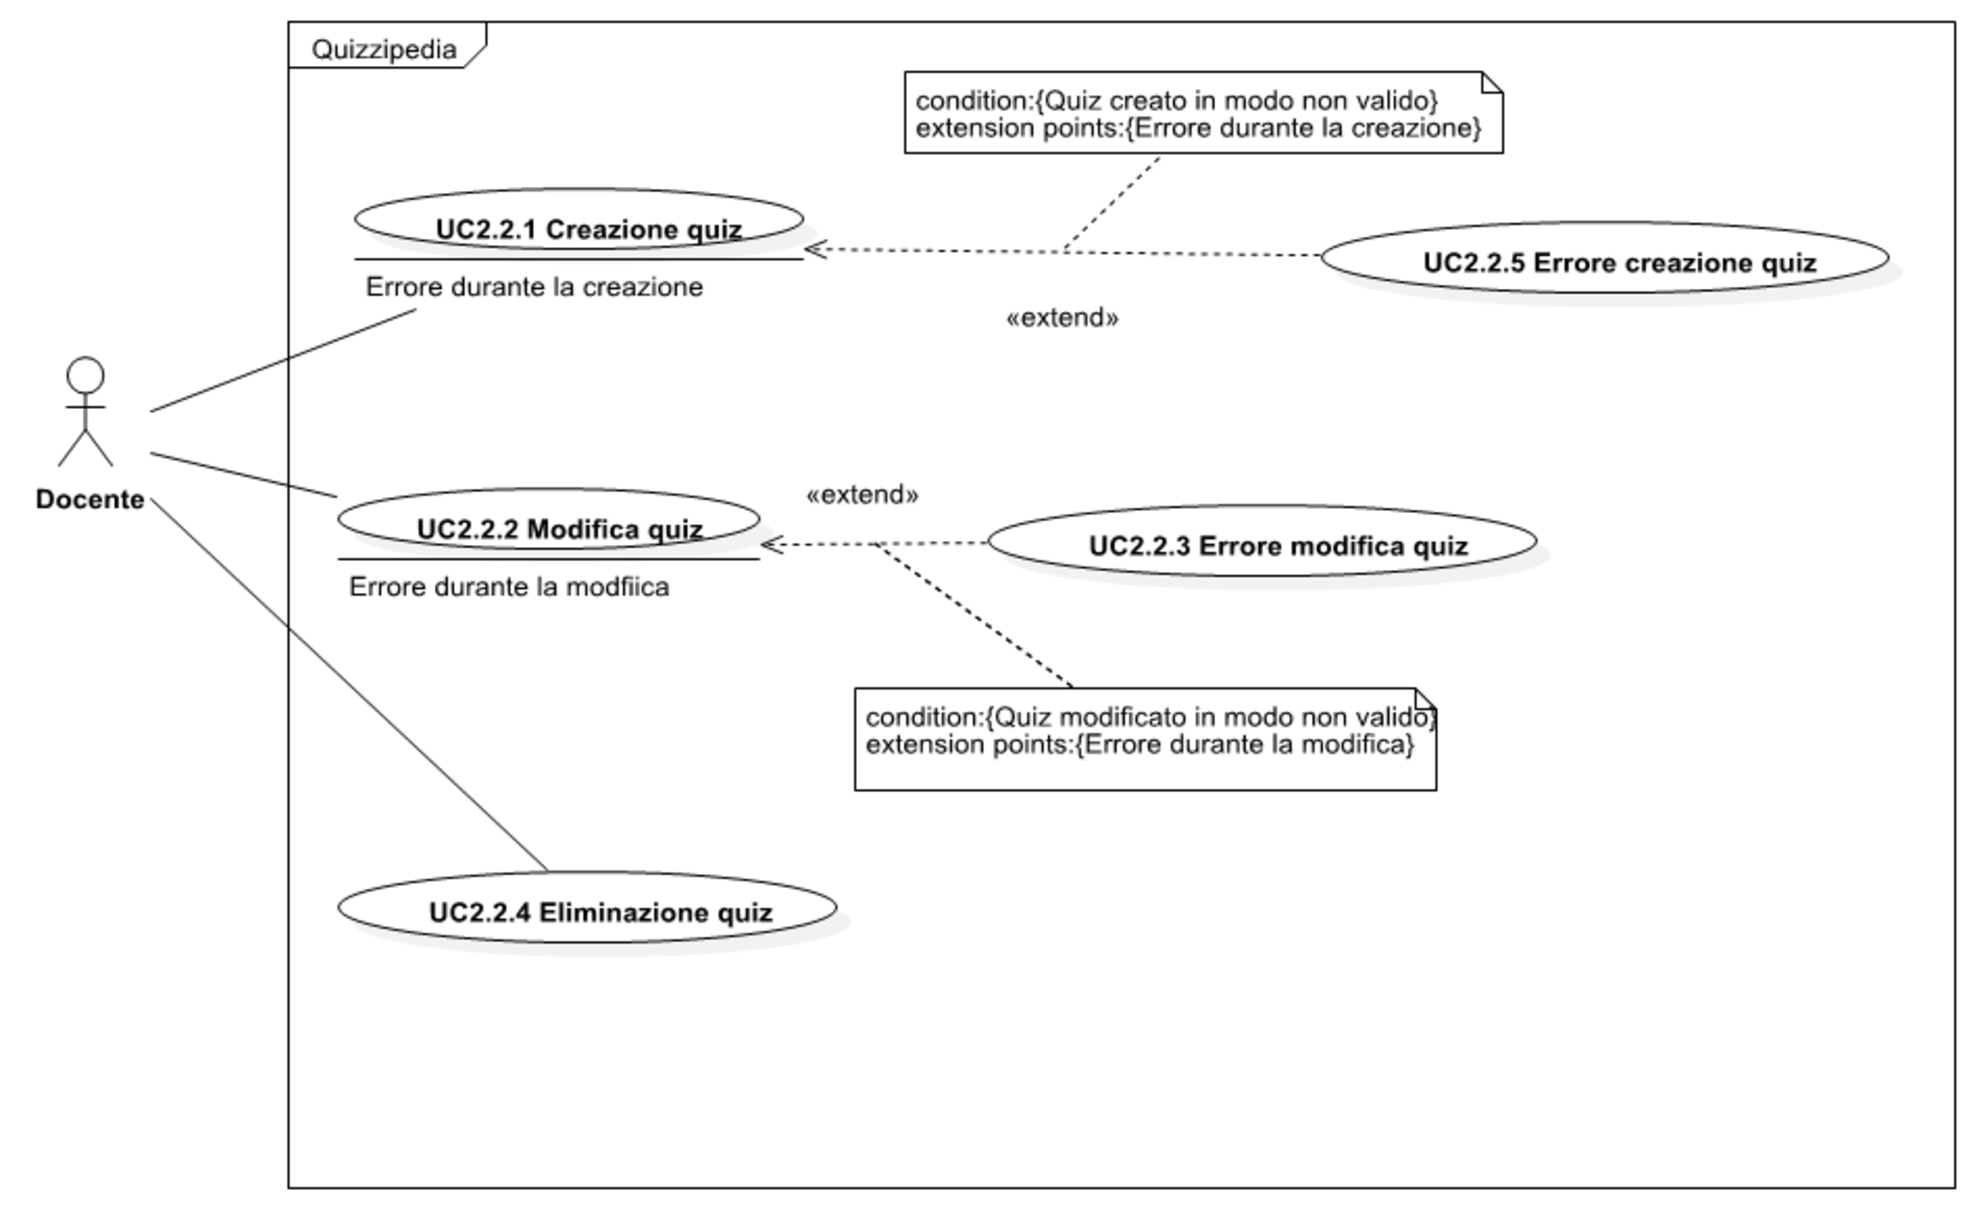
\includegraphics[width=\textwidth]{Img/UC Gestione quiz.pdf}}
\caption{UC2.2 Gestione quiz}
\end{figure}
\begin{itemize}
\item \textbf{Attori}: Docente.
\item \textbf{Scenario principale}:
\begin{enumerate}
\item Creazione quiz (UC2.2.1);
\item Modifica quiz (UC2.2.2);
\item Errore durante la modifica del quiz (UC2.2.3);
\item Eliminazione quiz (UC2.2.4);
\item Interruzione volontaria della creazione del quiz (UC2.2.5);
\item Interruzione volontaria della modifica del quiz (UC2.2.6);
\item Errore durante la creazione del quiz (UC2.2.7).
\end{enumerate}
\item \textbf{Descrizione}: il docente deve poter effettuare varie operazioni di gestione di quiz, in particolare deve poter creare quiz nuovi e modificare o eliminare quiz esistenti.
\item \textbf{Precondizione}: il docente è autenticato nel sistema e desidera effettuare operazioni sui quiz.
\item \textbf{Postcondizione}: il docente ha effettuato le operazioni desiderate sui quiz.
\end{itemize}
\subsubsection{UC2.2.1 Creazione quiz}
\begin{figure}[H]
\centering
\noindent\makebox[\textwidth]{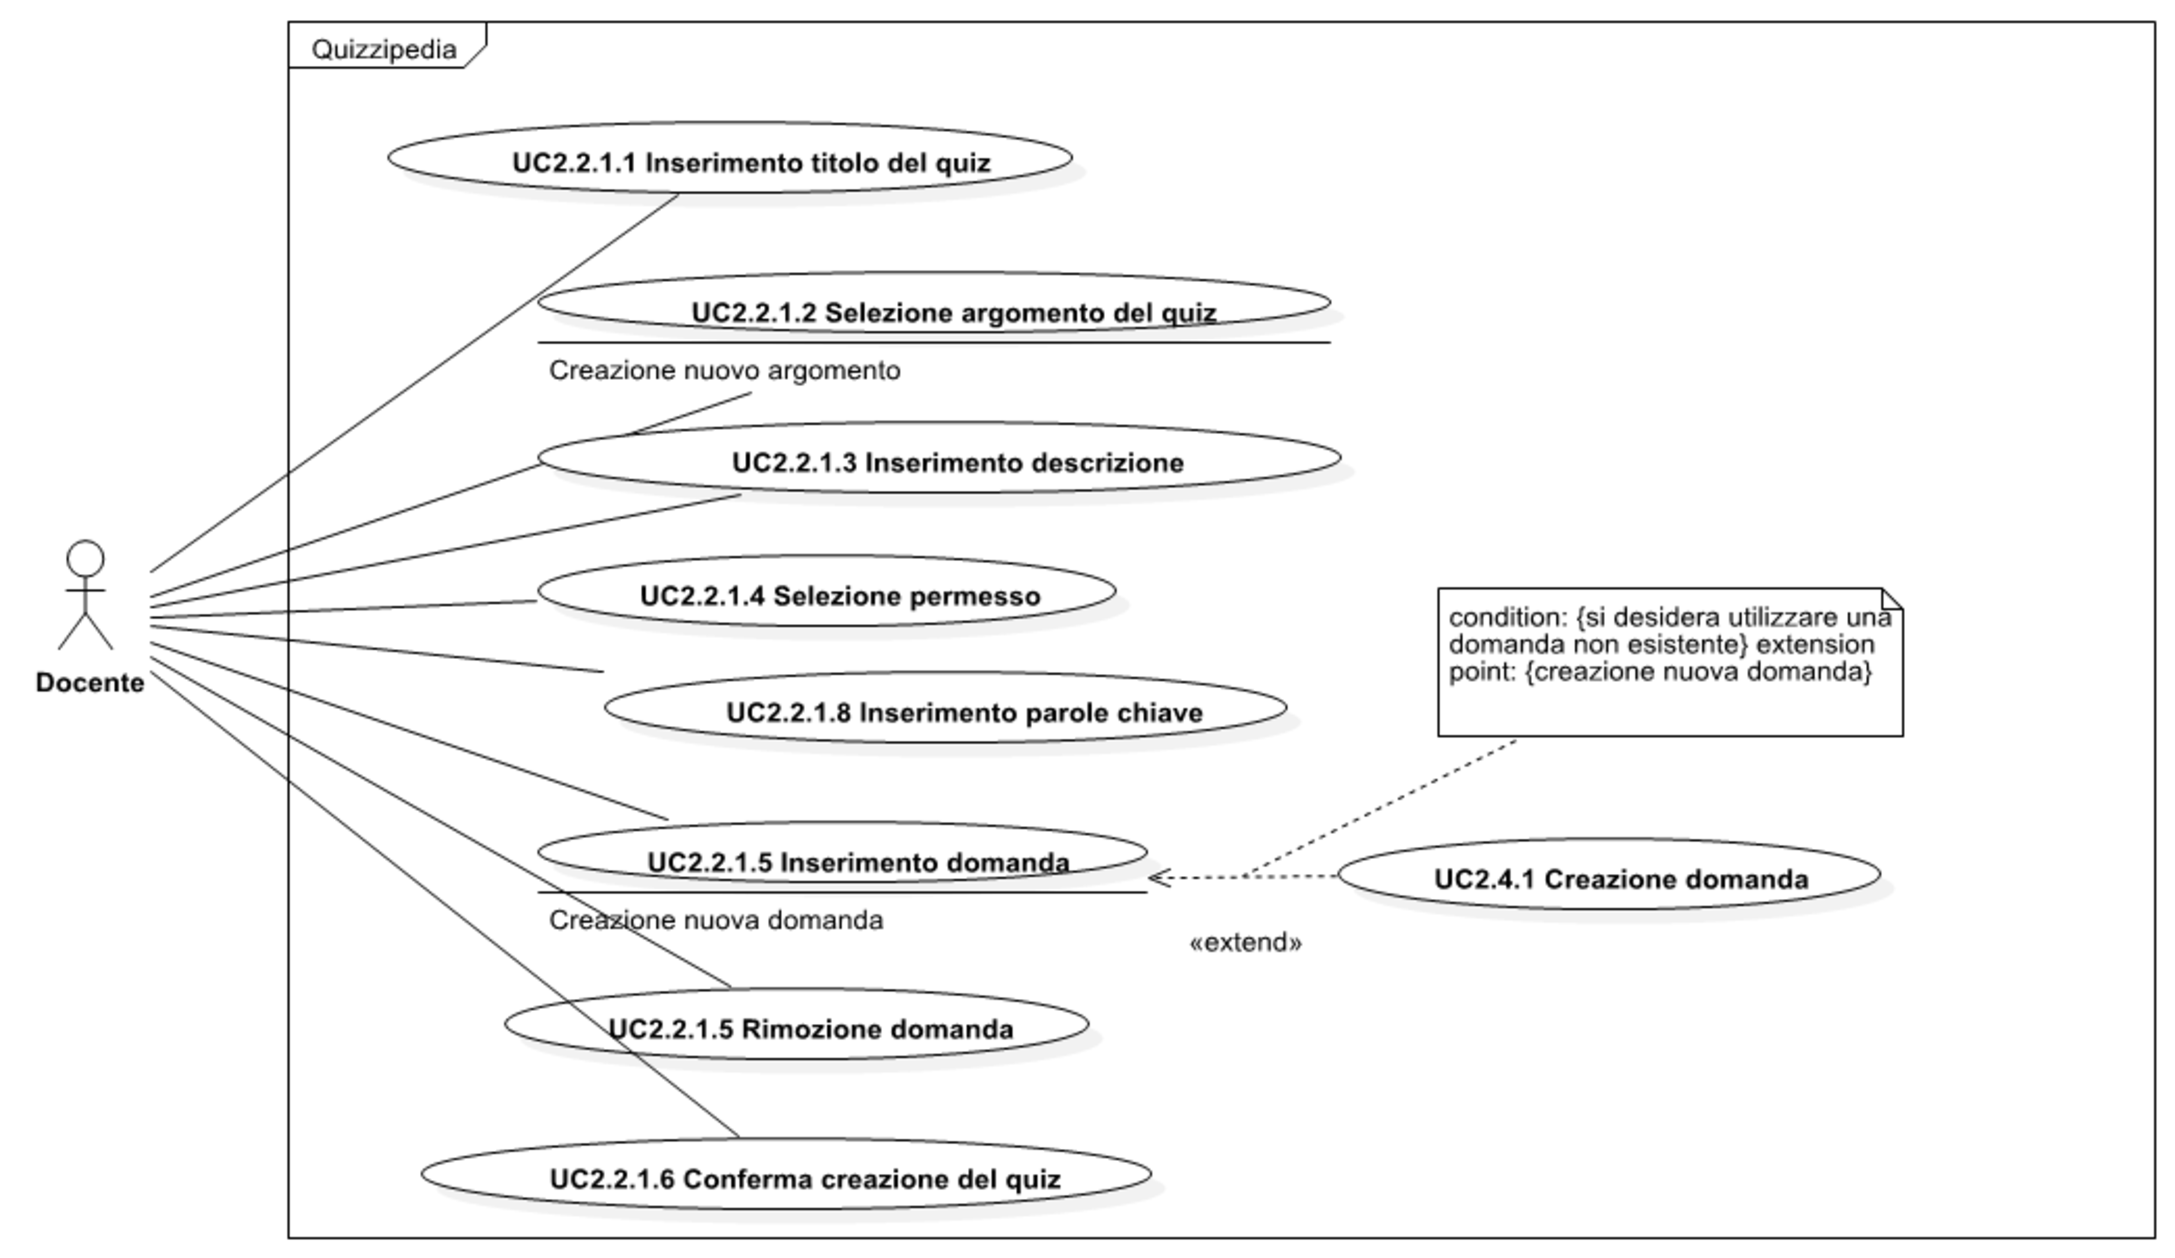
\includegraphics[width=\textwidth]{Img/UC Creazione quiz.pdf}}
\caption{UC2.2.1 Creazione quiz}
\end{figure}
\begin{itemize}
\item \textbf{Attori}: Docente.
\item \textbf{Scenario principale}:
\begin{enumerate}
\item Inserimento titolo del quiz (UC2.2.1.1);
\item Selezione argomento del quiz (UC2.2.1.2);
\item Inserimento descrizione (UC2.2.1.3);
\item Selezione permesso (UC2.2.1.4);
\item Inserimento domanda nel quiz (UC2.2.1.5);
\item Rimozione domanda dal quiz (UC2.2.1.6);
\item Conferma creazione quiz (UC2.2.1.7);
\item Inserimento parole chiave (UC2.2.1.8).
\end{enumerate}
\item \textbf{Estensioni}:
\begin{itemize}
\item Interruzione volontaria della creazione del quiz (UC2.2.5).
\end{itemize}
\item \textbf{Descrizione}: il docente deve poter creare un nuovo quiz.
\item \textbf{Precondizione}: il docente è autenticato nel sistema e desidera creare un nuovo quiz.
\item \textbf{Postcondizione}: il docente ha creato il nuovo quiz.
\end{itemize}
\subsubsection{UC2.2.1.1 Inserimento titolo del quiz}
\begin{itemize}
\item \textbf{Attori}: Docente.
\item \textbf{Scenario principale}: il docente inserisce il titolo del quiz.
\item \textbf{Descrizione}: il docente deve poter inserire il titolo del quiz che sta creando.
\item \textbf{Precondizione}: il docente sta creando un nuovo quiz e deve ancora inserire il titolo.
\item \textbf{Postcondizione}: il docente ha inserito il titolo del quiz.
\end{itemize}
\subsubsection{UC2.2.1.2 Selezione argomento del quiz}
\begin{itemize}
\item \textbf{Attori}: Docente.
\item \textbf{Scenario principale}: il docente deleziona l'argomento del quiz.
\item \textbf{Descrizione}: il docente deve poter selezionare l'argomento del quiz da una lista di argomenti, o creare un nuovo argomento se è mancante.
\item \textbf{Precondizione}: il docente sta creando un nuovo quiz e deve selezionare l'argomento.
\item \textbf{Postcondizione}: il docente ha selezionato l'argomento del quiz.
\end{itemize}
\subsubsection{UC2.2.1.3 Inserimento descrizione}
\begin{itemize}
\item \textbf{Attori}: Docente.
\item \textbf{Scenario principale}: il docente inserisce la descrizione del quiz.
\item \textbf{Descrizione}: il docente deve poter inserire la descrizione del quiz che sta creando.
\item \textbf{Precondizione}: il docente sta creando un nuovo quiz e deve ancora inserire la descrizione.
\item \textbf{Postcondizione}: il docente ha inserito la descrizione del quiz.
\end{itemize}
\subsubsection{UC2.2.1.4 Selezione permesso}
\begin{figure}[H]
\centering
\noindent\makebox[\textwidth]{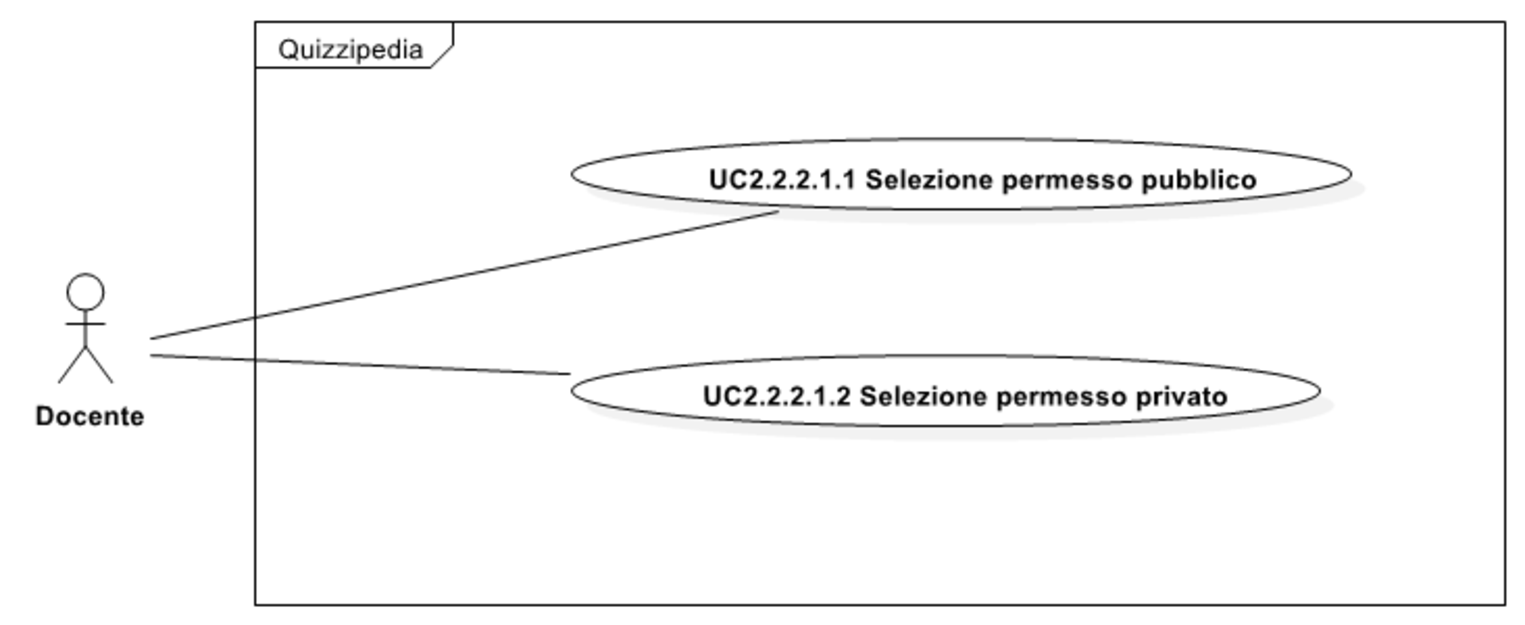
\includegraphics[width=\textwidth]{Img/UC Selezione permesso.pdf}}
\caption{UC2.2.1.4 Selezione permesso}
\end{figure}
\begin{itemize}
\item \textbf{Attori}: Docente.
\item \textbf{Scenario principale}:
\begin{enumerate}
\item Selezione permesso pubblico (UC2.2.1.4.1);
\item Selezione permesso privato (UC2.2.1.4.2).
\end{enumerate}
\item \textbf{Descrizione}: il docente deve selezionare il permesso del quiz.
\item \textbf{Precondizione}: il docente sta creando un nuovo quiz e deve ancora selezionarne il permesso.
\item \textbf{Postcondizione}: il docente ha selezionato il permesso del quiz.
\end{itemize}
\subsubsection{UC2.2.1.4.1 Selezione permesso pubblico}
\begin{itemize}
\item \textbf{Attori}: Docente.
\item \textbf{Scenario principale}: il docente seleziona il permesso 'pubblico'.
\item \textbf{Descrizione}: il docente deve poter selezionare il permesso 'pubblico' per il quiz.
\item \textbf{Precondizione}: il docente sta selezionando il permesso del quiz che sta creando.
\item \textbf{Postcondizione}: il docente ha selezionato il permesso 'pubblico'.
\end{itemize}
\subsubsection{UC2.2.1.4.2 Selezione permesso privato}
\begin{figure}[H]
\centering
\noindent\makebox[\textwidth]{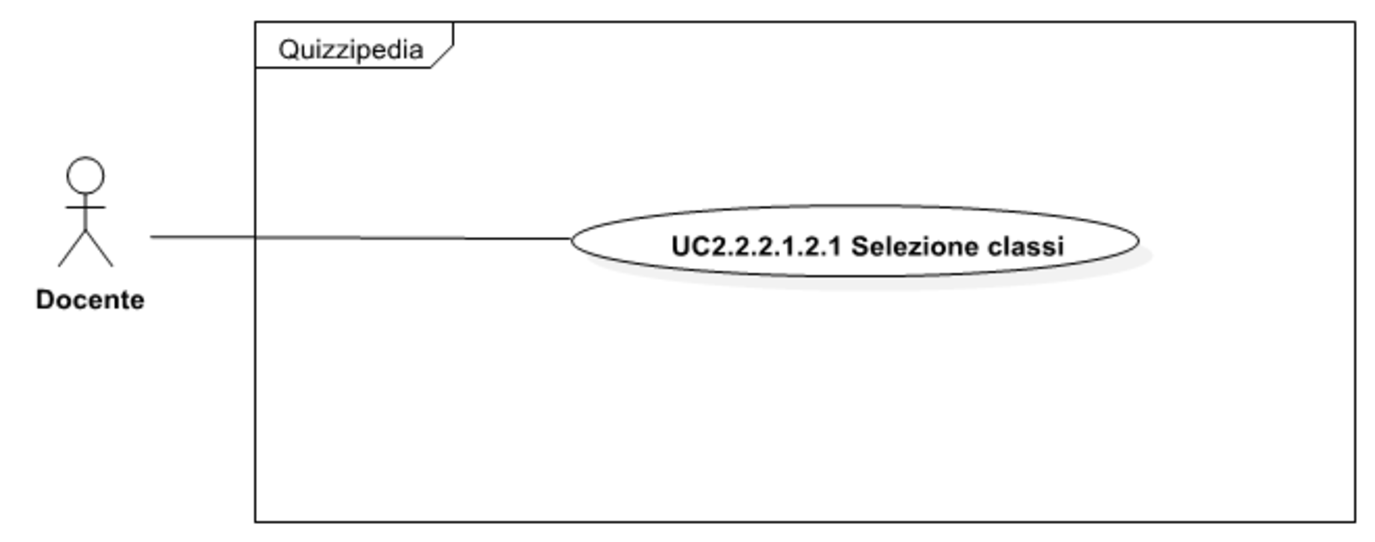
\includegraphics[width=\textwidth]{Img/UC Selezione permesso privato.pdf}}
\caption{UC2.2.1.4.2 Selezione permesso privato}
\end{figure}
\begin{itemize}
\item \textbf{Attori}: Docente.
\item \textbf{Scenario principale}:
\begin{enumerate}
\item Selezione classi (UC2.2.1.4.2.1).
\end{enumerate}
\item \textbf{Descrizione}: il docente deve poter selezionare il permesso 'privato' per il quiz.
\item \textbf{Precondizione}: il docente sta selezionando il permesso del quiz che sta creando.
\item \textbf{Postcondizione}: il docente ha selezionato il permesso 'privato'.
\end{itemize}
\subsubsection{UC2.2.1.4.2.1 Selezione classi}
\begin{itemize}
\item \textbf{Attori}: Docente.
\item \textbf{Scenario principale}: il docente seleziona le classi a cui assegnare il quiz privato.
\item \textbf{Descrizione}: il docente può assegnare il quiz privato a una o più classi di studenti, i cui partecipanti avranno il diritto di svolgerlo.
\item \textbf{Precondizione}: il docente ha selezionato il permesso 'privato' per il quiz che sta creando.
\item \textbf{Postcondizione}: il docente ha assegnato le classi a cui assegnare il quiz che sta creando.
\end{itemize}
\subsubsection{UC2.2.1.5 Inserimento domanda nel quiz}
\begin{itemize}
\item \textbf{Attori}: Docente.
\item \textbf{Scenario principale}: il docente inserisce una domanda nel quiz.
\item \textbf{Descrizione}: il docente deve poter inserire una domanda nel quiz.
\item \textbf{Precondizione}: il docente sta creando un quiz e vuole inserire una domanda.
\item \textbf{Postcondizione}: il docente ha inserito la domanda nel quiz.
\end{itemize}
\subsubsection{UC2.2.1.6 Rimozione domanda dal quiz}
\begin{itemize}
\item \textbf{Attori}: Docente.
\item \textbf{Scenario principale}: il docente rimuove una domanda dal quiz.
\item \textbf{Descrizione}: il docente deve poter rimuovere una domanda dal quiz (la domanda non sarà cancellata ma soltanto rimossa dal quiz).
\item \textbf{Precondizione}: il docente sta creando un quiz e vuole rimuovere una domanda.
\item \textbf{Postcondizione}: il docente ha rimosso la domanda.
\end{itemize}
\subsubsection{UC2.2.1.7 Conferma creazione quiz}
\begin{itemize}
\item \textbf{Attori}: Docente.
\item \textbf{Scenario principale}: il docente conferma la creazione del quiz.
\item \textbf{Descrizione}: il docente deve confermare la creazione del nuovo quiz per portarla a termine.
\item \textbf{Precondizione}: il docente sta creando un nuovo quiz e deve ancora confermare la sua creazione.
\item \textbf{Postcondizione}: il docente ha confermato la creazione del quiz.
\end{itemize}
\subsubsection{UC2.2.1.8 Inserimento parole chiave}
\begin{itemize}
\item \textbf{Attori}: Docente.
\item \textbf{Scenario principale}: il docente specifica le parole chiave del quiz.
\item \textbf{Descrizione}: il docente deve poter specificare le parole chiave del quiz durante la sua creazione.
\item \textbf{Precondizione}: il docente sta creando un quiz.
\item \textbf{Postcondizione}: il docente ha specificato le parole chiave del quiz.
\end{itemize}
\subsubsection{UC2.2.2 Modifica quiz}
\begin{figure}[H]
\centering
\noindent\makebox[\textwidth]{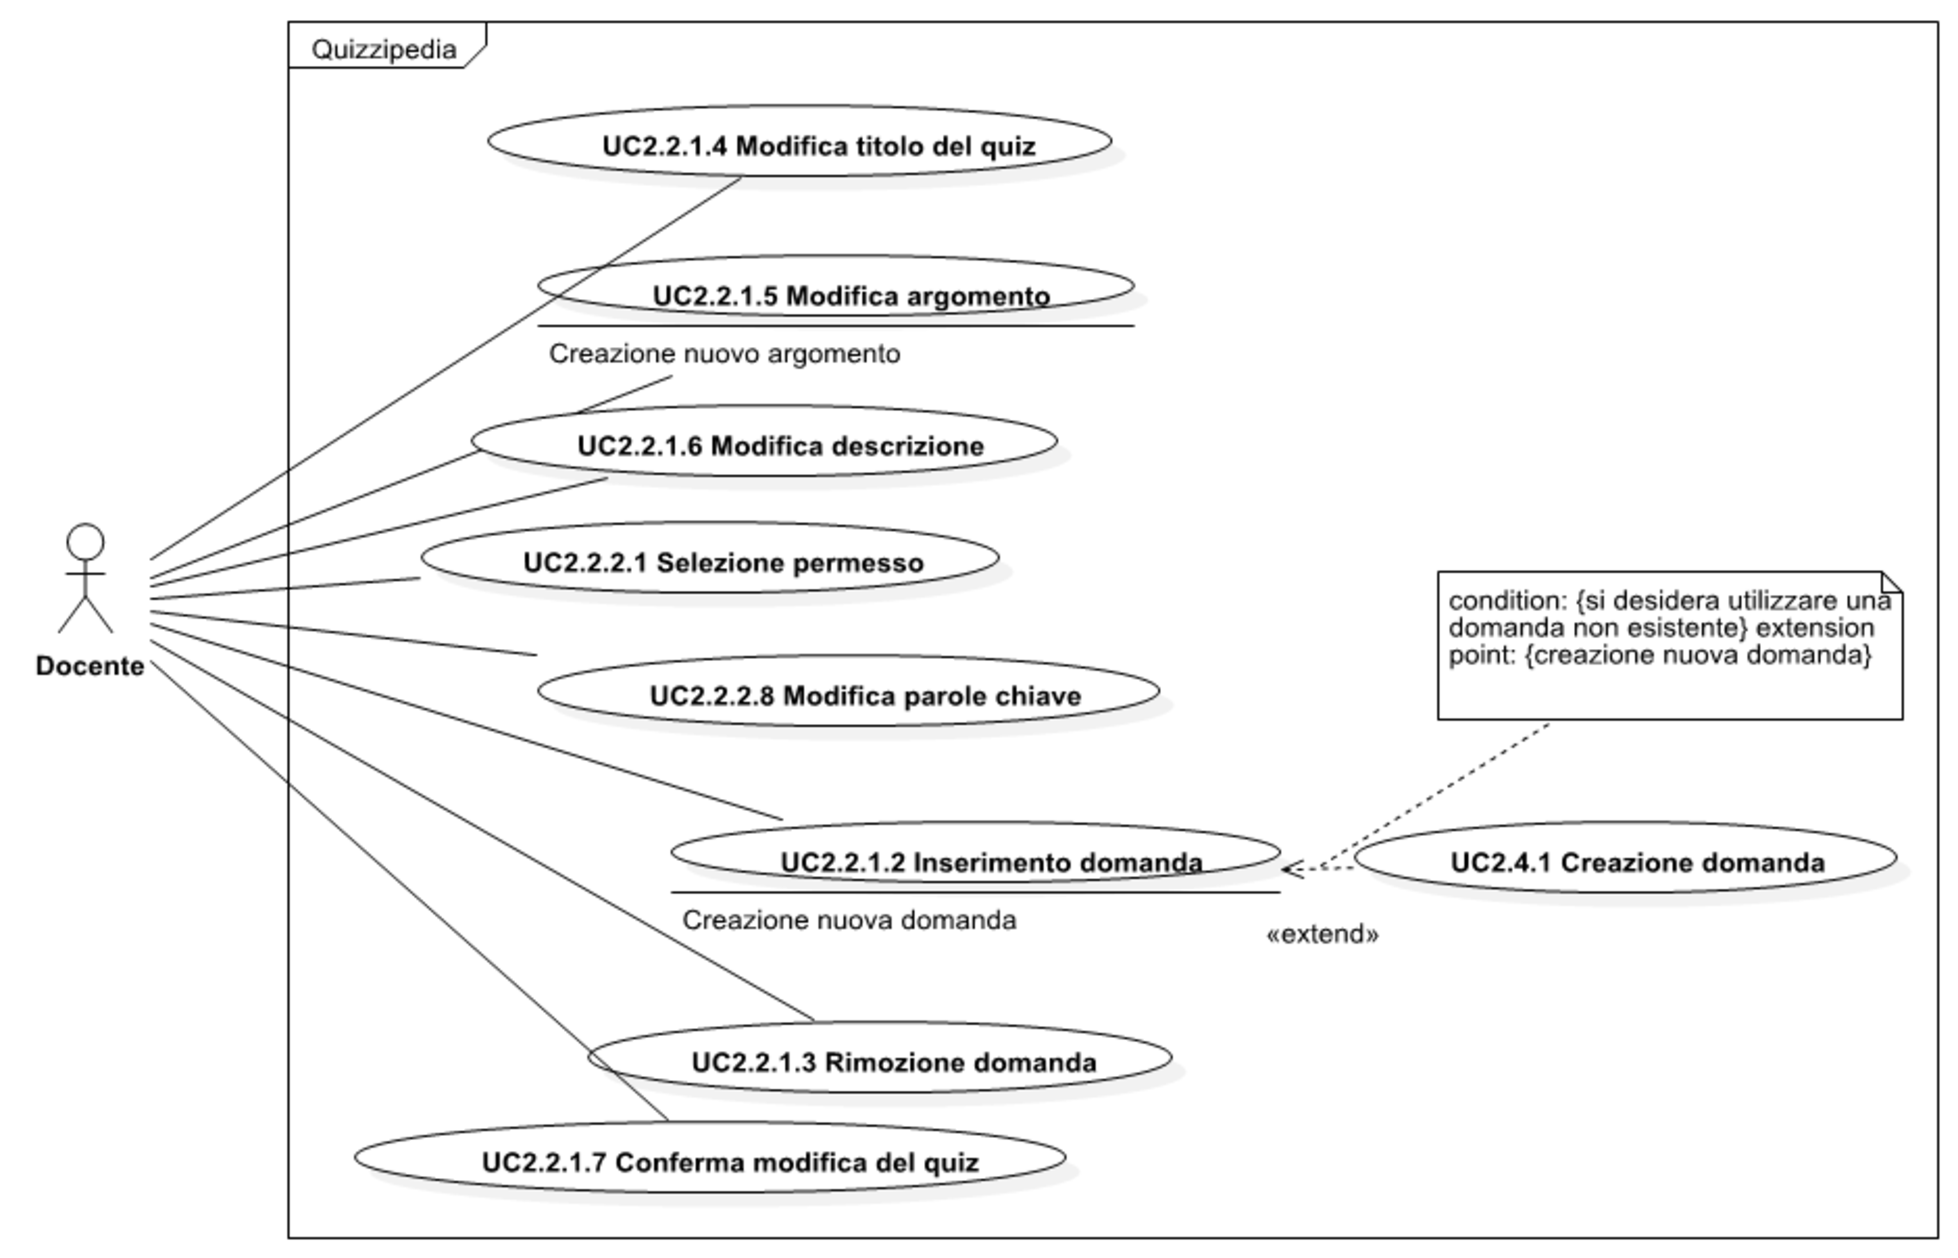
\includegraphics[width=\textwidth]{Img/UC Modifica quiz.pdf}}
\caption{UC2.2.2 Modifica quiz}
\end{figure}
\begin{itemize}
\item \textbf{Attori}: Docente.
\item \textbf{Scenario principale}:
\begin{enumerate}
\item Selezione permesso (UC2.2.2.1);
\item Inserimento domanda nel quiz (UC2.2.2.2);
\item Rimozione domanda dal quiz (UC2.2.2.3);
\item Modifica titolo del quiz (UC2.2.2.4);
\item Modifica argomento del quiz (UC2.2.2.5);
\item Modifica descrizione (UC2.2.2.6);
\item Conferma modifica quiz (UC2.2.2.7);
\item Modifica parole chiave (UC2.2.2.8).
\end{enumerate}
\item \textbf{Estensioni}:
\begin{itemize}
\item Errore durante la modifica del quiz (UC2.2.3);
\item Interruzione volontaria della modifica del quiz (UC2.2.6).
\end{itemize}
\item \textbf{Descrizione}: il docente deve poter modificare un quiz.
\item \textbf{Precondizione}: il docente è autenticato nel sistema e desidera modificare un quiz.
\item \textbf{Postcondizione}: il docente ha modificato il quiz.
\end{itemize}
\subsubsection{UC2.2.2.1 Selezione permesso}
\begin{figure}[H]
\centering
\noindent\makebox[\textwidth]{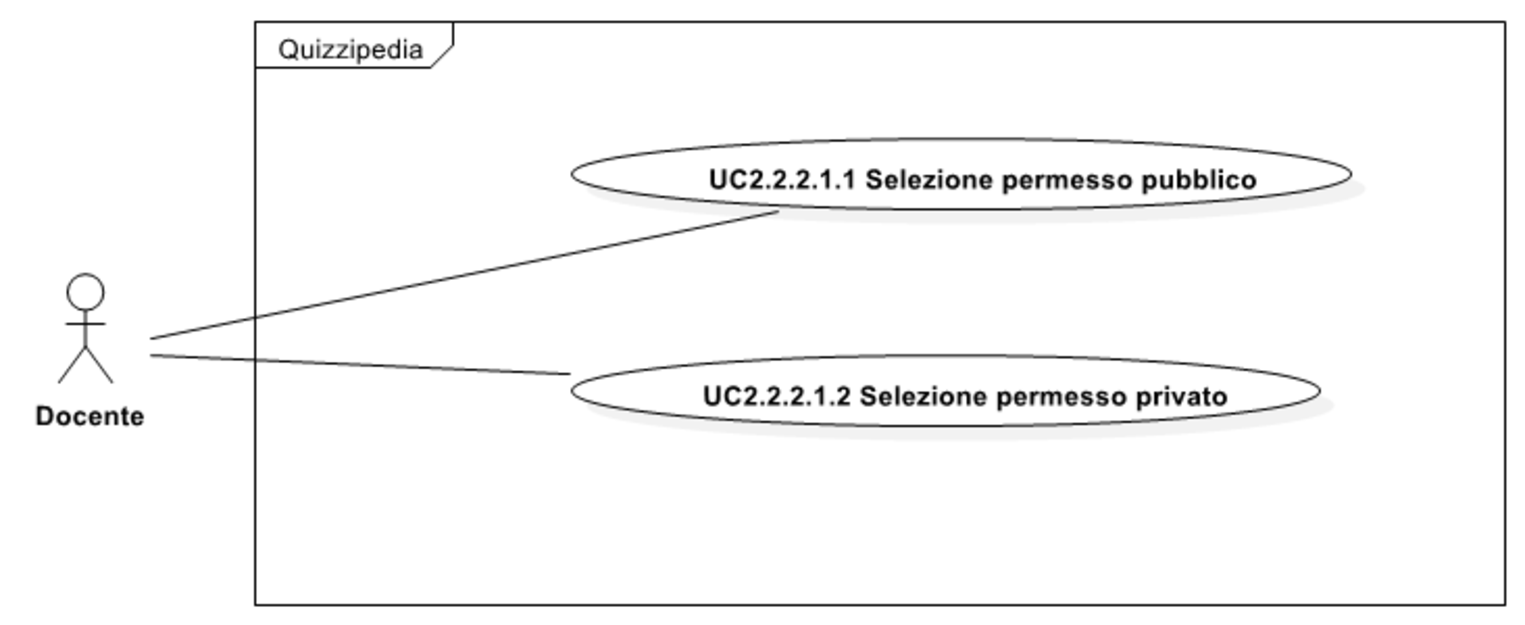
\includegraphics[width=\textwidth]{Img/UC Selezione permesso.pdf}}
\caption{UC2.2.2.1 Selezione permesso}
\end{figure}
\begin{itemize}
\item \textbf{Attori}: Docente.
\item \textbf{Scenario principale}:
\begin{enumerate}
\item Selezione permesso pubblico (UC2.2.2.1.1);
\item Selezione permesso privato (UC2.2.2.1.2).
\end{enumerate}
\item \textbf{Descrizione}: il docente deve poter scegliere il permesso del quiz.
\item \textbf{Precondizione}: il docente sta modificando un quiz.
\item \textbf{Postcondizione}: il docente ha specificato il permesso del quiz.
\end{itemize}
\subsubsection{UC2.2.2.1.1 Selezione permesso pubblico}
\begin{itemize}
\item \textbf{Attori}: Responsabile.
\item \textbf{Scenario principale}: il docente seleziona il permesso 'pubblico' per il quiz.
\item \textbf{Descrizione}: il docente ha scelto un permesso 'pubblico' per il quiz, permettendo a tutti gli utenti di svolgerlo senza restrizioni.
\item \textbf{Precondizione}: il docente sta selezionando il permesso di un quiz.
\item \textbf{Postcondizione}: il docente ha scelto il permesso 'pubblico'.
\end{itemize}
\subsubsection{UC2.2.2.1.2 Selezione permesso privato}
\begin{figure}[H]
\centering
\noindent\makebox[\textwidth]{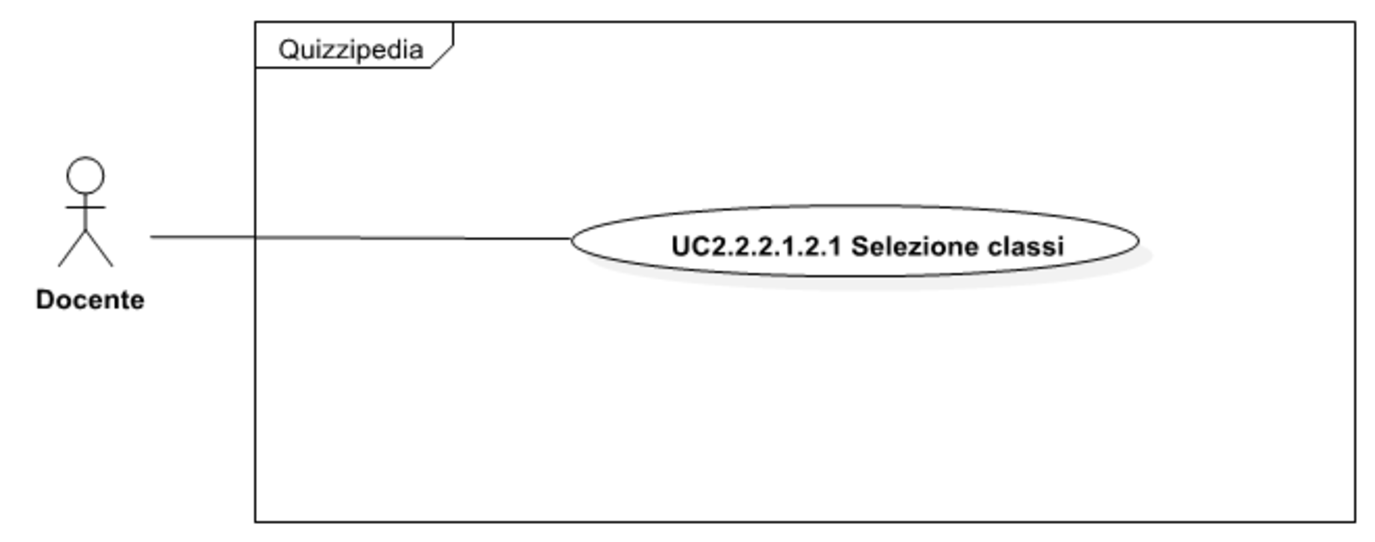
\includegraphics[width=\textwidth]{Img/UC Selezione permesso privato.pdf}}
\caption{UC2.2.2.1.2 Selezione permesso privato}
\end{figure}
\begin{itemize}
\item \textbf{Attori}: Docente.
\item \textbf{Scenario principale}:
\begin{enumerate}
\item Selezione classi (UC2.2.2.1.2.1).
\end{enumerate}
\item \textbf{Descrizione}: il docente ha scelto un permesso privato per il quiz, limitando il suo accesso e svolgimento a una cerchia ristretta di studenti.
\item \textbf{Precondizione}: il docente sta selezionando il permesso di un quiz.
\item \textbf{Postcondizione}: il docente ha scelto il permesso privato.
\end{itemize}
\subsubsection{UC2.2.2.1.2.1 Selezione classi}
\begin{itemize}
\item \textbf{Attori}: Docente.
\item \textbf{Scenario principale}: il docente seleziona le classi a cui assegnare il quiz privato.
\item \textbf{Descrizione}: il docente può assegnare il quiz privato a una o più classi di studenti, i cui partecipanti avranno diritto di svolgerlo.
\item \textbf{Precondizione}: il docente ha selezionato il permesso 'privato' per il quiz che sta modificando.
\item \textbf{Postcondizione}: il docente ha selezionato le classi a cui assegnare il quiz che sta modificando.
\end{itemize}
\subsubsection{UC2.2.2.2 Inserimento domanda nel quiz}
\begin{itemize}
\item \textbf{Attori}: Docente.
\item \textbf{Scenario principale}: il docente inserisce una domanda nel quiz.
\item \textbf{Descrizione}: il docente deve poter inserire una domanda nel quiz.
\item \textbf{Precondizione}: il docente sta modificando un quiz e vuole inserire una domanda.
\item \textbf{Postcondizione}: il docente ha inserito la domanda.
\end{itemize}
\subsubsection{UC2.2.2.3 Rimozione domanda dal quiz}
\begin{itemize}
\item \textbf{Attori}: Docente.
\item \textbf{Scenario principale}: il docente rimuove una domanda dal quiz.
\item \textbf{Descrizione}: il docente deve poter rimuovere una domanda nel quiz (la domanda non sarà cancellata ma soltanto rimossa dal quiz).
\item \textbf{Precondizione}: il docente sta modificando il quiz e vuole rimuovere una domanda.
\item \textbf{Postcondizione}: il docente ha rimosso la domanda.
\end{itemize}
\subsubsection{UC2.2.2.4 Modifica titolo del quiz}
\begin{itemize}
\item \textbf{Attori}: Docente.
\item \textbf{Scenario principale}: il docente modifica il titolo del quiz.
\item \textbf{Descrizione}: il docente deve poter modificare il titolo del quiz.
\item \textbf{Precondizione}: il docente sta modificando un nuovo quiz.
\item \textbf{Postcondizione}: il docente ha modificato il titolo del quiz.
\end{itemize}
\subsubsection{UC2.2.2.5 Modifica argomento del quiz}
\begin{itemize}
\item \textbf{Attori}: Docente.
\item \textbf{Scenario principale}: il docente modifica l'argomento del quiz.
\item \textbf{Estensioni}:
\begin{itemize}
\item Creazione argomento (UC2.3.1).
\end{itemize}
\item \textbf{Descrizione}: il docente deve poter selezionare l'argomento del quiz da una lista di argomenti, o creare un nuovo argomento se è mancante.
\item \textbf{Precondizione}: il docente sta modificando un quiz.
\item \textbf{Postcondizione}: il docente ha modificato l'argomento del quiz.
\end{itemize}
\subsubsection{UC2.2.2.6 Modifica descrizione}
\begin{itemize}
\item \textbf{Attori}: Docente.
\item \textbf{Scenario principale}: il docente modifica la descrizione del quiz.
\item \textbf{Descrizione}: il docente deve poter modificare la descrizione del quiz.
\item \textbf{Precondizione}: il docente sta modificando un quiz.
\item \textbf{Postcondizione}: il docente ha modificato la descrizione del quiz.
\end{itemize}
\subsubsection{UC2.2.2.7 Conferma modifica quiz}
\begin{itemize}
\item \textbf{Attori}: Docente.
\item \textbf{Scenario principale}: il docente conferma la modifica del quiz.
\item \textbf{Descrizione}: il docente deve confermare la modifica del quiz per portarla a termine.
\item \textbf{Precondizione}: il docente sta modificando un quiz e deve ancora confermare la sua modifica.
\item \textbf{Postcondizione}: il docente ha confermato la modifica del quiz.
\end{itemize}
\subsubsection{UC2.2.2.8 Modifica parole chiave}
\begin{itemize}
\item \textbf{Attori}: Docente.
\item \textbf{Scenario principale}: il docente modifica le parole chiave del quiz.
\item \textbf{Descrizione}: il docente deve poter modificare le parole chiave del quiz durante la sua modifica.
\item \textbf{Precondizione}: il docente sta modificando le parole chiave del quiz.
\item \textbf{Postcondizione}: il docente ha modificato le parole chiave del quiz.
\end{itemize}
\subsubsection{UC2.2.3 Errore durante la modifica del quiz}
\begin{itemize}
\item \textbf{Attori}: Docente.
\item \textbf{Scenario principale}: il docente visualizza il messaggio di errore.
\item \textbf{Descrizione}: il docente ha modificato il quiz in modo non valido.
\item \textbf{Precondizione}: si è verificata una delle seguenti condizioni: numero di domande scorretto; campi obbligatori lasciati vuoti.
\item \textbf{Postcondizione}: il docente ha visualizzato il messaggio di errore.
\end{itemize}
\subsubsection{UC2.2.4 Eliminazione quiz}
\begin{figure}[H]
\centering
\noindent\makebox[\textwidth]{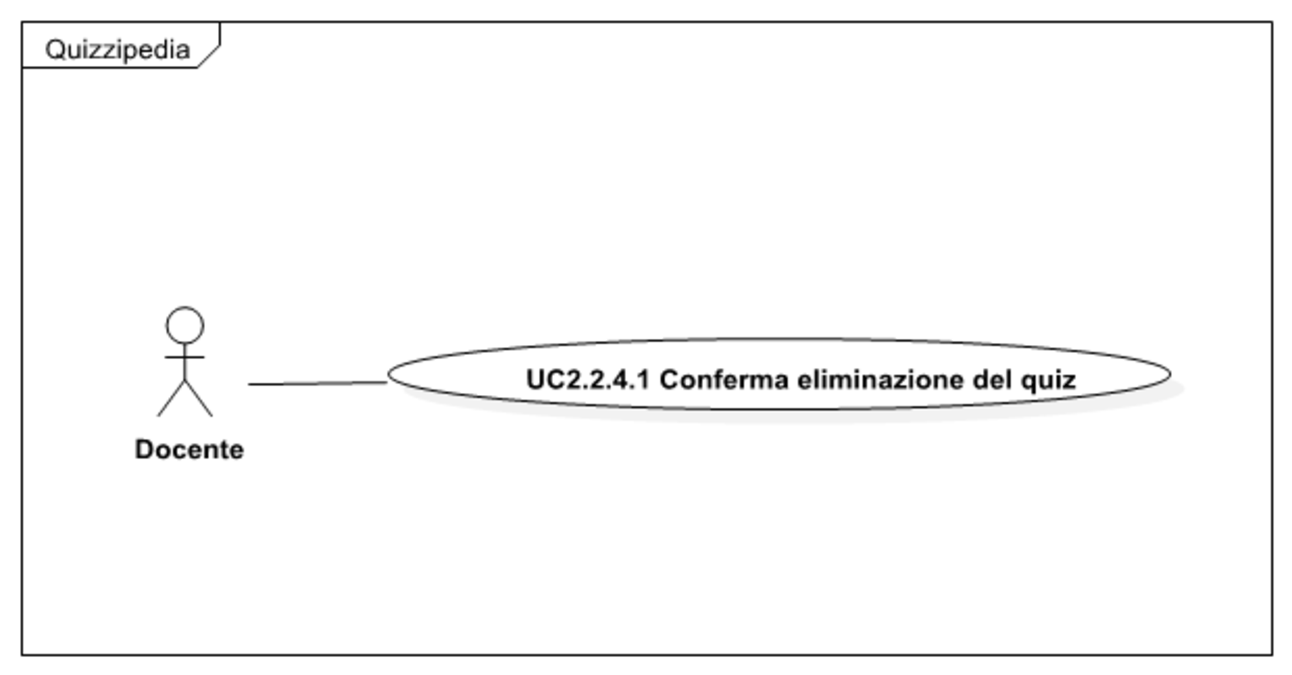
\includegraphics[width=\textwidth]{Img/UC Eliminazione quiz.pdf}}
\caption{UC2.2.4 Eliminazione quiz}
\end{figure}
\begin{itemize}
\item \textbf{Attori}: Docente.
\item \textbf{Scenario principale}:
\begin{enumerate}
\item Conferma eliminazione del quiz (UC2.2.4.1).
\end{enumerate}
\item \textbf{Descrizione}: il docente deve poter eliminare un quiz. Questo non causerà l’eliminazione delle domande contenute nel quiz.
\item \textbf{Precondizione}: il docente è autenticato nel sistema e desidera eliminare un quiz esistente.
\item \textbf{Postcondizione}: il docente ha eliminato il quiz.
\end{itemize}
\subsubsection{UC2.2.4.1 Conferma eliminazione del quiz}
\begin{itemize}
\item \textbf{Attori}: Docente.
\item \textbf{Scenario principale}: il docente conferma l'eliminazione del quiz.
\item \textbf{Descrizione}: il docente dovrà confermare l'eliminazione del quiz.
\item \textbf{Precondizione}: il docente ha richiesto l'eliminazione di un quiz e deve ancora effettuare la conferma.
\item \textbf{Postcondizione}: il docente ha confermato l'eliminazione del quiz.
\end{itemize}
\subsubsection{UC2.2.5 Interruzione volontaria della creazione del quiz}
\begin{itemize}
\item \textbf{Attori}: Docente.
\item \textbf{Scenario principale}: il docente interrompe la creazione del quiz.
\item \textbf{Descrizione}: Il docente interrompe la creazione del quiz.
\item \textbf{Precondizione}: Il docente sta creando un quiz.
\item \textbf{Postcondizione}: Il docente non completa la creazione del quiz.
\end{itemize}
\subsubsection{UC2.2.6 Interruzione volontaria della modifica del quiz}
\begin{itemize}
\item \textbf{Attori}: Docente.
\item \textbf{Scenario principale}: il docente interrompe la modifica del quiz.
\item \textbf{Descrizione}: Il docente interrompe la modifica del quiz.
\item \textbf{Precondizione}: Il docente sta modificando un quiz.
\item \textbf{Postcondizione}: Il docente non ha completato la modifica del quiz.
\end{itemize}
\subsubsection{UC2.2.7 Errore durante la creazione del quiz}
\begin{itemize}
\item \textbf{Attori}: Docente.
\item \textbf{Scenario principale}: il docente visualizza un messaggio di errore.
\item \textbf{Descrizione}: il docente ha creato un quiz non valido.
\item \textbf{Precondizione}: si è verificata una delle seguenti condizioni nella creazione del quiz: numero di domande scorretto; campi obbligatori lasciati vuoti.
\item \textbf{Postcondizione}: il docente ha visualizzato il messaggio di errore.
\end{itemize}
\subsubsection{UC2.3 Gestione argomenti}
\begin{figure}[H]
\centering
\noindent\makebox[\textwidth]{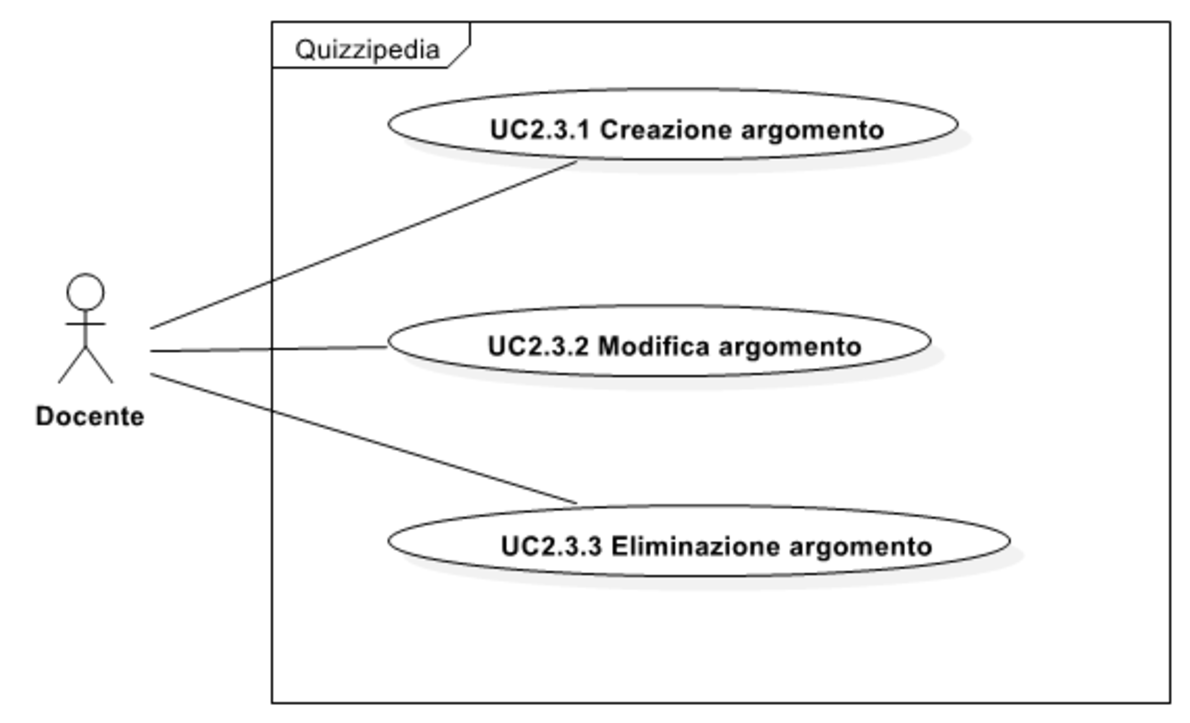
\includegraphics[width=\textwidth]{Img/UC Gestione argomenti.pdf}}
\caption{UC2.3 Gestione argomenti}
\end{figure}
\begin{itemize}
\item \textbf{Attori}: Responsabile.
\item \textbf{Scenario principale}:
\begin{enumerate}
\item Creazione argomento (UC2.3.1);
\item Rimozione argomento (UC2.3.2).
\end{enumerate}
\item \textbf{Descrizione}: il responsabile  deve poter gestire gli argomenti di quiz e domande, in particolare può inserire nuovi argomenti e eliminare argomenti esistenti.
\item \textbf{Precondizione}: il responsabile è autenticato e desidera effettuare operazioni sugli argomenti.
\item \textbf{Postcondizione}: il responsabile ha effettuato le operazioni sugli argomenti.
\end{itemize}
\subsubsection{UC2.3.1 Creazione argomento}
\begin{figure}[H]
\centering
\noindent\makebox[\textwidth]{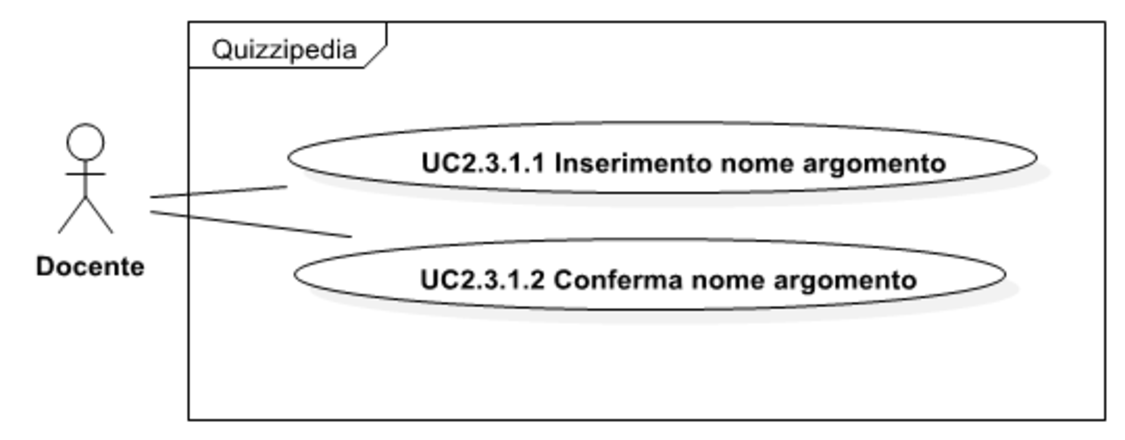
\includegraphics[width=\textwidth]{Img/UC Creazione argomento.pdf}}
\caption{UC2.3.1 Creazione argomento}
\end{figure}
\begin{itemize}
\item \textbf{Attori}: Responsabile.
\item \textbf{Scenario principale}:
\begin{enumerate}
\item Inserimento nome argomento (UC2.3.1.1);
\item Conferma creazione argomento (UC2.3.1.2).
\end{enumerate}
\item \textbf{Descrizione}: il responsabile deve poter creare un nuovo argomento.
\item \textbf{Precondizione}: il responsabile è autenticato e vuole creare un nuovo argomento.
\item \textbf{Postcondizione}: il responsabile ha creato il nuovo argomento.
\end{itemize}
\subsubsection{UC2.3.1.1 Inserimento nome argomento}
\begin{itemize}
\item \textbf{Attori}: Responsabile.
\item \textbf{Scenario principale}: il docente inserisce il nome dell'argomento.
\item \textbf{Descrizione}: il docente deve poter inserire il nome dell'argomento.
\item \textbf{Precondizione}: il docente sta creando un nuovo argomento e deve ancora inserire il nome.
\item \textbf{Postcondizione}: il docente ha inserito il nome dell'argomento.
\end{itemize}
\subsubsection{UC2.3.1.2 Conferma creazione argomento}
\begin{itemize}
\item \textbf{Attori}: Responsabile.
\item \textbf{Scenario principale}: il docente conferma la creazione dell'argomento.
\item \textbf{Descrizione}: il docente deve poter confermare la creazione dell'argomento.
\item \textbf{Precondizione}: il docente ha inserito un nuovo argomento e deve ancora confermare.
\item \textbf{Postcondizione}: il docente ha confermato il nuovo argomento.
\end{itemize}
\subsubsection{UC2.3.2 Rimozione argomento}
\begin{figure}[H]
\centering
\noindent\makebox[\textwidth]{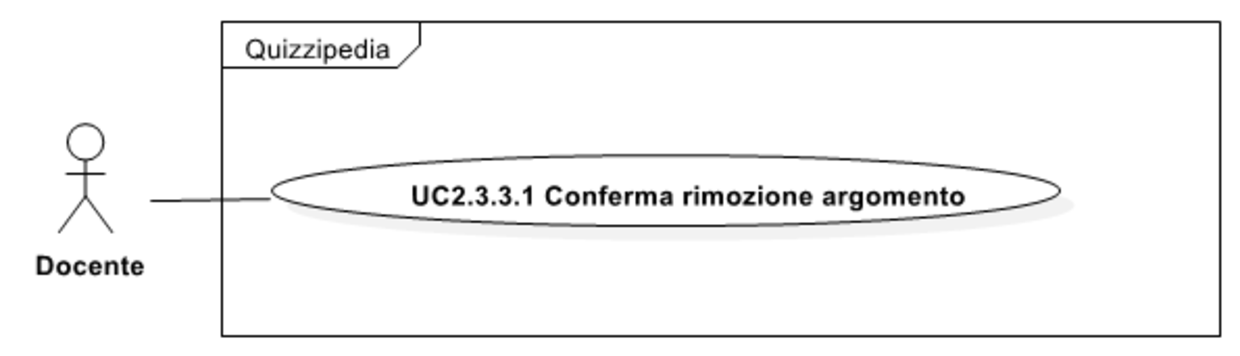
\includegraphics[width=\textwidth]{Img/UC Rimozione argomento.pdf}}
\caption{UC2.3.2 Rimozione argomento}
\end{figure}
\begin{itemize}
\item \textbf{Attori}: Responsabile.
\item \textbf{Scenario principale}:
\begin{enumerate}
\item Conferma rimozione argomento (UC2.3.2.1).
\end{enumerate}
\item \textbf{Descrizione}: il responsabile deve poter rimuovere un argomento.
\item \textbf{Precondizione}: il responsabile è nella gestione degli argomenti e vuole eliminare un argomento.
\item \textbf{Postcondizione}: il responsabile ha eliminato l'argomento.
\end{itemize}
\subsubsection{UC2.3.2.1 Conferma rimozione argomento}
\begin{itemize}
\item \textbf{Attori}: Responsabile.
\item \textbf{Scenario principale}: il responsabile conferma la rimozione dell'argomento.
\item \textbf{Descrizione}: il responsabile deve poter confermare la rimozione dell'argomento.
\item \textbf{Precondizione}: il responsabile ha selezionato l'argomento da eliminare e deve ancora confermare.
\item \textbf{Postcondizione}: il responsabile ha confermato l'eliminazione dell'argomento.
\end{itemize}
\subsubsection{UC2.4 Gestione account}
\begin{figure}[H]
\centering
\noindent\makebox[\textwidth]{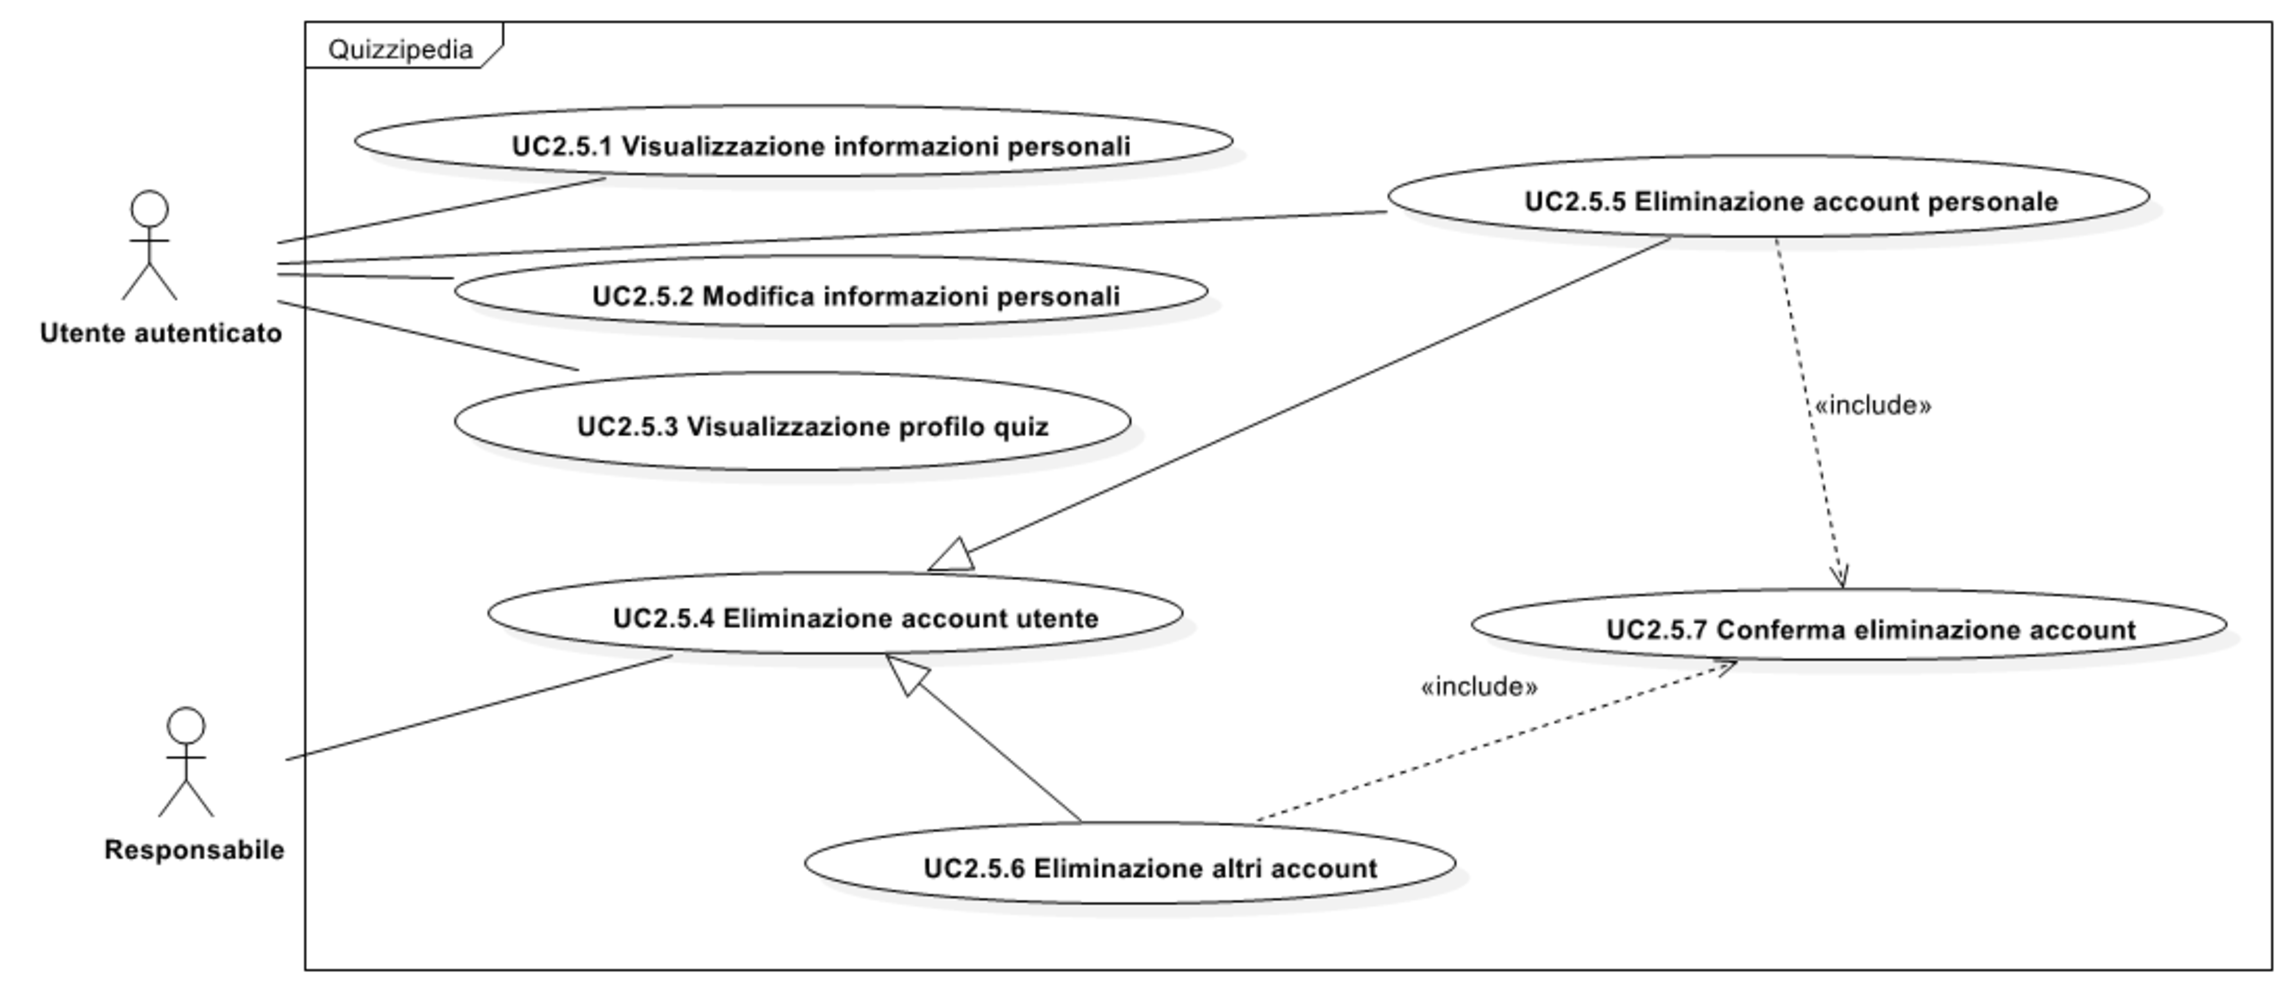
\includegraphics[width=\textwidth]{Img/UC Gestione account.pdf}}
\caption{UC2.4 Gestione account}
\end{figure}
\begin{itemize}
\item \textbf{Attori}: Responsabile, Utente Autenticato.
\item \textbf{Scenario principale}:
\begin{enumerate}
\item Visualizzazione informazioni personali (UC2.4.1);
\item Modifica informazioni personali (UC2.4.2);
\item Visualizzazione profilo quiz (UC2.4.3);
\item Eliminazione account (UC2.4.4);
\item Interruzione volontaria della modifica delle informazioni personali (UC2.4.5).
\end{enumerate}
\item \textbf{Descrizione}: L'utente autenticato può visualizzare e modificare le sue informazioni personali, visualizzare il proprio profilo quiz e la possibilità di eliminare il proprio account. Il responsabile in aggiunta può eliminare gli account degli utenti.
\item \textbf{Precondizione}: il responsabile o un utente autorizzato vuole modificare/visualizzare le informazioni del proprio account.
\item \textbf{Postcondizione}: l'utente autenticato o il responsabile hanno effettuato le modifiche opportune al proprio account.
\end{itemize}
\subsubsection{UC2.4.1 Visualizzazione informazioni personali}
\begin{figure}[H]
\centering
\noindent\makebox[\textwidth]{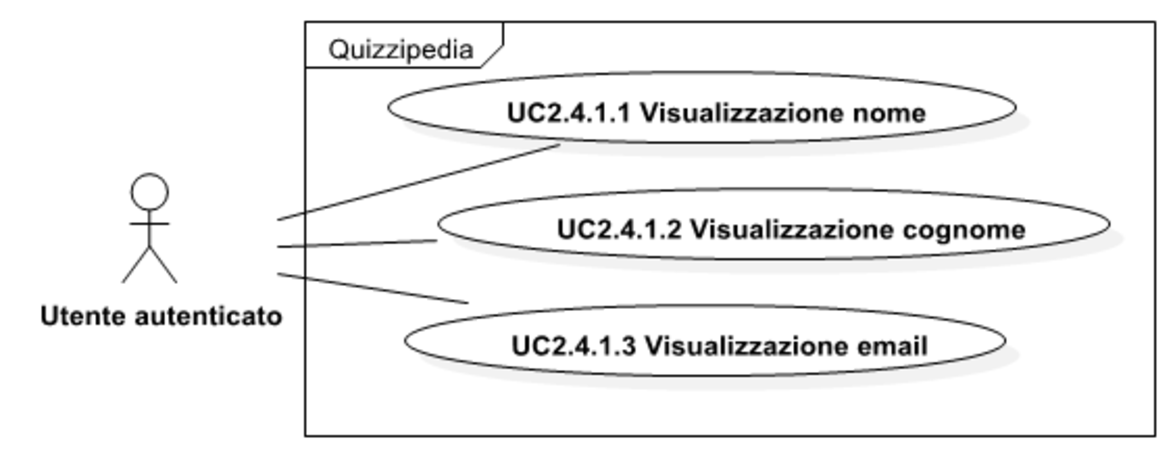
\includegraphics[width=\textwidth]{Img/UC Visualizzazione informazioni personali.pdf}}
\caption{UC2.4.1 Visualizzazione informazioni personali}
\end{figure}
\begin{itemize}
\item \textbf{Attori}: Utente Autenticato.
\item \textbf{Scenario principale}:
\begin{enumerate}
\item Visualizzazione nome (UC2.4.1.1);
\item Visualizzazione cognome (UC2.4.1.2);
\item Visualizzazione email (UC2.4.1.3).
\end{enumerate}
\item \textbf{Descrizione}: l’utente autenticato può visualizzare le sue informazioni personali.
\item \textbf{Precondizione}: l’utente autenticato ha l’accesso alla gestione dell’account.
\item \textbf{Postcondizione}: l’utente autenticato ha visualizzato le sue informazioni personali.
\end{itemize}
\subsubsection{UC2.4.1.1 Visualizzazione nome}
\begin{itemize}
\item \textbf{Attori}: Utente Autenticato.
\item \textbf{Scenario principale}: l'utente autenticato visualizza il proprio nome.
\item \textbf{Descrizione}: l'utente autenticato può visualizzare il suo nome.
\item \textbf{Precondizione}: l'utente è autenticato e sta visualizzando le sue informazioni personali.
\item \textbf{Postcondizione}: l'utente ha visualizzato il proprio nome.
\end{itemize}
\subsubsection{UC2.4.1.2 Visualizzazione cognome}
\begin{itemize}
\item \textbf{Attori}: Utente Autenticato.
\item \textbf{Scenario principale}: l'utente autenticato visualizza il proprio cognome.
\item \textbf{Descrizione}: l'utente autenticato può visualizzare il suo cognome.
\item \textbf{Precondizione}: l'utente è autenticato e sta visualizzando le sue informazioni personali.
\item \textbf{Postcondizione}: l'utente ha visualizzato il proprio cognome.
\end{itemize}
\subsubsection{UC2.4.1.3 Visualizzazione email}
\begin{itemize}
\item \textbf{Attori}: Utente Autenticato.
\item \textbf{Scenario principale}: l'utente autenticato visualizza il proprio indirizzo email.
\item \textbf{Descrizione}: l'utente autenticato può visualizzare la sua email.
\item \textbf{Precondizione}: l'utente è autenticato e sta visualizzando le sue informazioni personali.
\item \textbf{Postcondizione}: l'utente ha visualizzato la propria email.
\end{itemize}
\subsubsection{UC2.4.2 Modifica informazioni personali}
\begin{figure}[H]
\centering
\noindent\makebox[\textwidth]{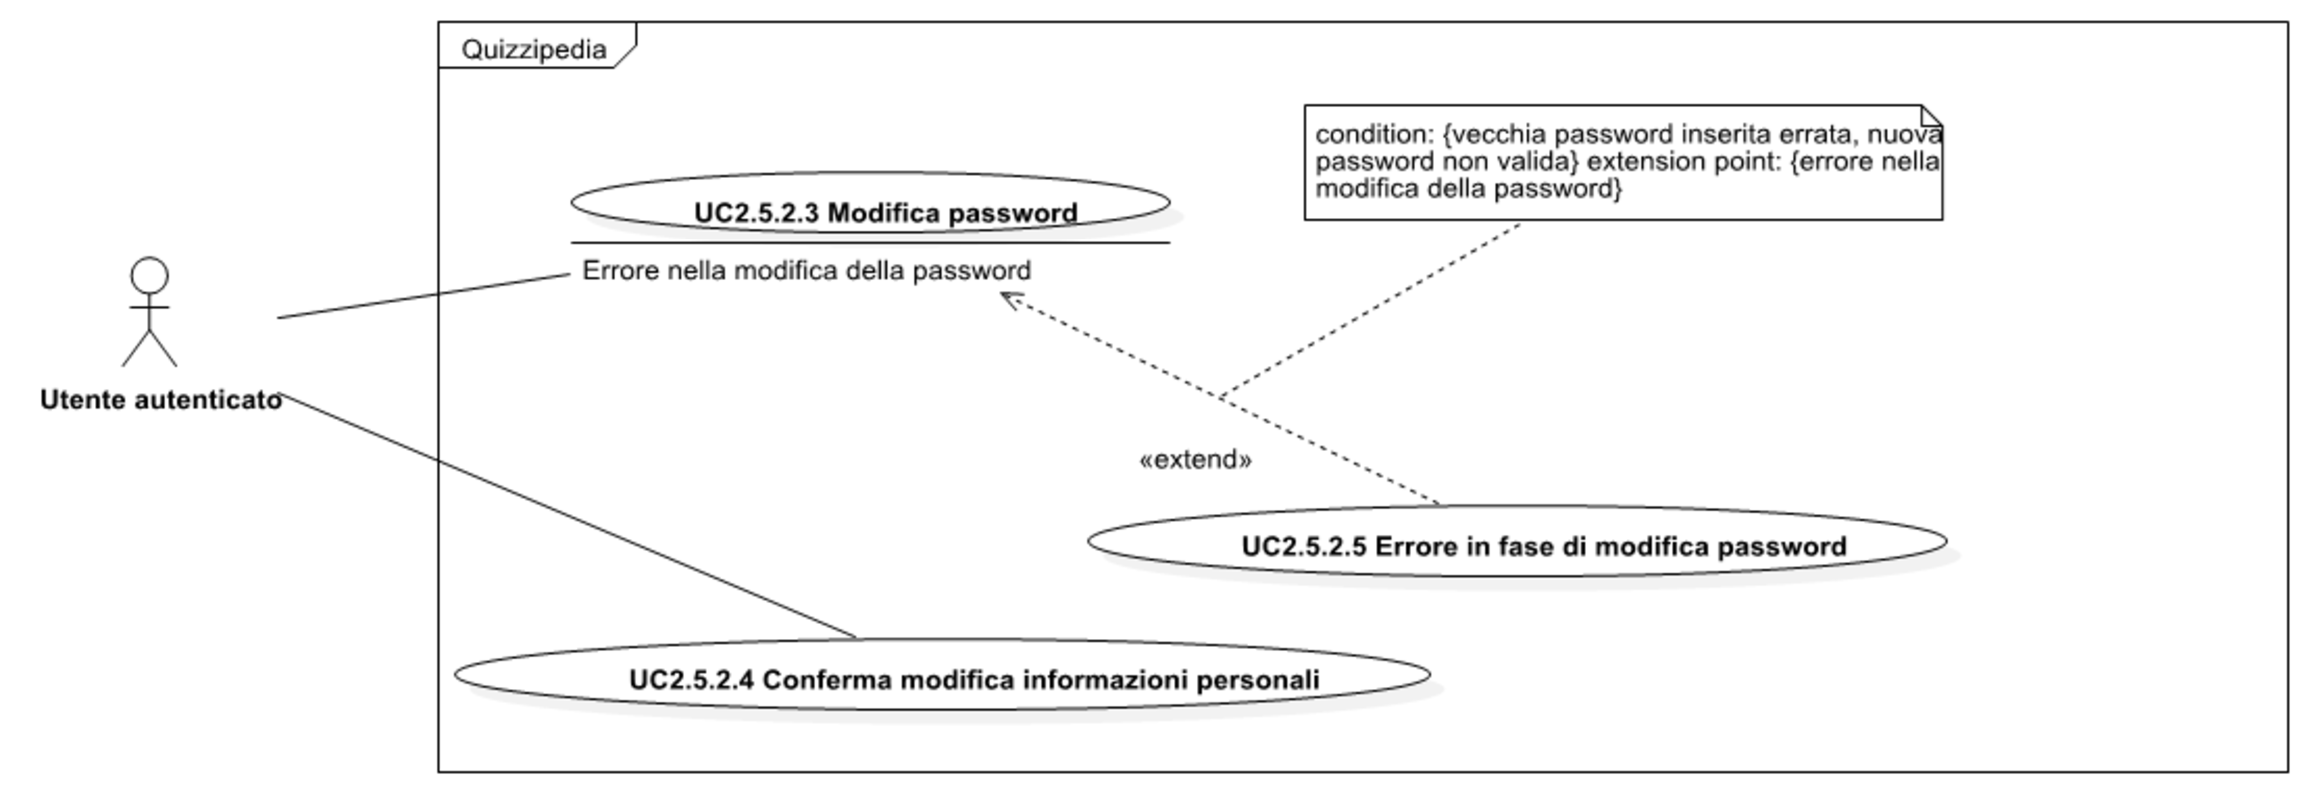
\includegraphics[width=\textwidth]{Img/UC Modifica informazioni personali.pdf}}
\caption{UC2.4.2 Modifica informazioni personali}
\end{figure}
\begin{itemize}
\item \textbf{Attori}: Utente Autenticato.
\item \textbf{Scenario principale}:
\begin{enumerate}
\item Modifica password (UC2.4.2.1);
\item Errore modifica password (UC2.4.2.2);
\item Conferma modifica informazioni personali (UC2.4.2.3).
\end{enumerate}
\item \textbf{Estensioni}:
\begin{itemize}
\item Interruzione volontaria della modifica delle informazioni personali (UC2.4.5).
\end{itemize}
\item \textbf{Descrizione}: l'utente autenticato vuole modificare le sue informazioni personali.
\item \textbf{Precondizione}: l'utente autenticato può modificare le sue informazioni personali.
\item \textbf{Postcondizione}: l'utente ha modificato le sue informazioni personali.
\end{itemize}
\subsubsection{UC2.4.2.1 Modifica password}
\begin{figure}[H]
\centering
\noindent\makebox[\textwidth]{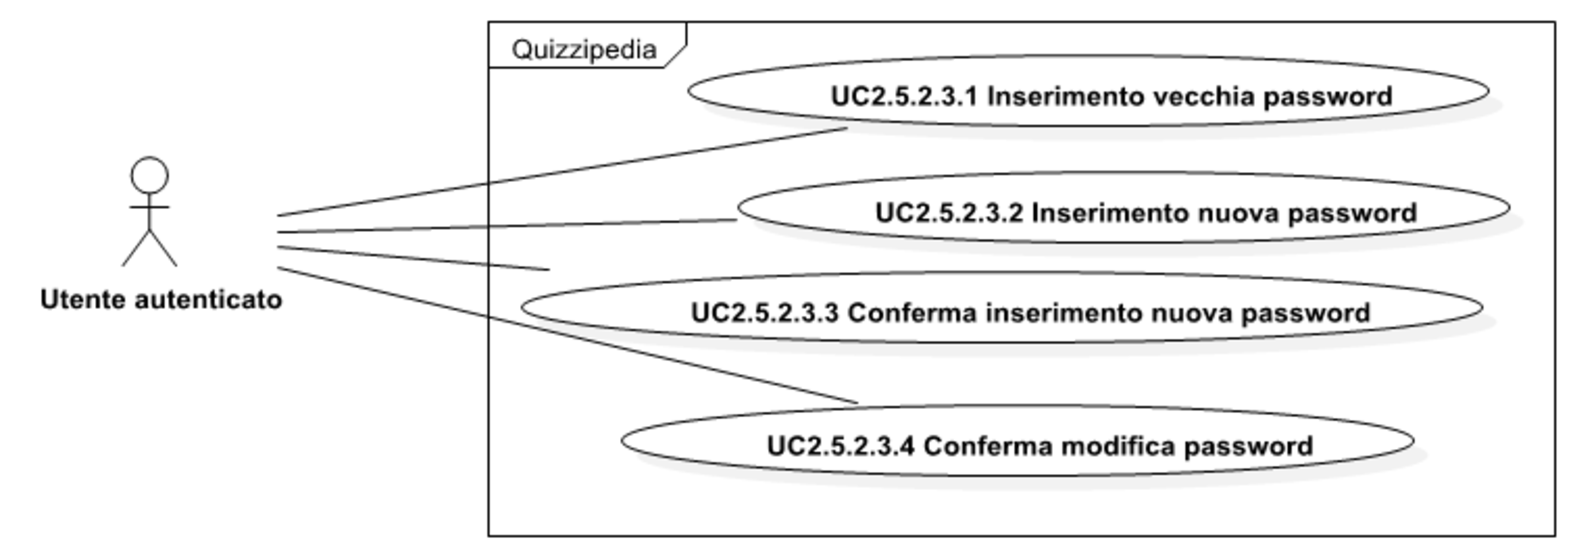
\includegraphics[width=\textwidth]{Img/UC Modifica password.pdf}}
\caption{UC2.4.2.1 Modifica password}
\end{figure}
\begin{itemize}
\item \textbf{Attori}: Utente Autenticato.
\item \textbf{Scenario principale}:
\begin{enumerate}
\item Inserimento vecchia password (UC2.4.2.1.1);
\item Inserimento nuova password (UC2.4.2.1.2);
\item Conferma inserimento nuova password (UC2.4.2.1.3);
\item Conferma modifica password (UC2.4.2.1.4).
\end{enumerate}
\item \textbf{Estensioni}:
\begin{itemize}
\item Errore modifica password (UC2.4.2.2).
\end{itemize}
\item \textbf{Descrizione}: l'utente autenticato può modificare la sua password.
\item \textbf{Precondizione}: l'utente autenticato modifica le sue informazioni personali.
\item \textbf{Postcondizione}: l'utente ha modificato la sua password.
\end{itemize}
\subsubsection{UC2.4.2.1.1 Inserimento vecchia password}
\begin{itemize}
\item \textbf{Attori}: Utente Autenticato.
\item \textbf{Scenario principale}: l'utente autenticato inserisce la sua vecchia password.
\item \textbf{Descrizione}: la modifica della password richiede l'inserimento della password corrente o di una password temporanea.
\item \textbf{Precondizione}: l'utente autenticato ha deciso di modificare la password e deve ancora inserire la vecchia password.
\item \textbf{Postcondizione}: l'utente autenticato ha inserito la vecchia password.
\end{itemize}
\subsubsection{UC2.4.2.1.2 Inserimento nuova password}
\begin{itemize}
\item \textbf{Attori}: Utente Autenticato.
\item \textbf{Scenario principale}: l'utente autenticato inserisce la nuova password.
\item \textbf{Descrizione}: la modifica della password richiede l'inserimento della nuova password.
\item \textbf{Precondizione}: l'utente autenticato ha deciso di modificare la password e deve ancora inserire la nuova password.
\item \textbf{Postcondizione}: l'utente autenticato ha inserito la nuova password.
\end{itemize}
\subsubsection{UC2.4.2.1.3 Conferma inserimento nuova password}
\begin{itemize}
\item \textbf{Attori}: Utente Autenticato.
\item \textbf{Scenario principale}: l'utente autenticato conferma l'inserimento della nuova password.
\item \textbf{Descrizione}: la modifica della password richiede la conferma dell'inserimento della nuova password.
\item \textbf{Precondizione}: l'utente autenticato ha deciso di modificare la password e deve ancora confermare l'inserimento della nuova password.
\item \textbf{Postcondizione}: l'utente autenticato ha confermato l'inserimento della nuova password.
\end{itemize}
\subsubsection{UC2.4.2.1.4 Conferma modifica password}
\begin{itemize}
\item \textbf{Attori}: Utente Autenticato.
\item \textbf{Scenario principale}: l'utente autenticato conferma la modifica della password.
\item \textbf{Descrizione}: La modifica della password richiede la conferma della modifica password.
\item \textbf{Precondizione}: l'utente autenticato ha inserito i campi necessari e deve ancora confermare la modifica della password.
\item \textbf{Postcondizione}: l'utente autenticato ha confermato la modifica della password.
\end{itemize}
\subsubsection{UC2.4.2.2 Errore modifica password}
\begin{itemize}
\item \textbf{Attori}: Utente Autenticato.
\item \textbf{Scenario principale}: l'utente visualizza il messaggio di errore.
\item \textbf{Descrizione}: si è verificato un errore durante la modifica della password.
\item \textbf{Precondizione}: l'utente autenticato ha inserito una password non valida.
\item \textbf{Postcondizione}: l'utente visualizza un messaggio di errore.
\end{itemize}
\subsubsection{UC2.4.2.3 Conferma modifica informazioni personali}
\begin{itemize}
\item \textbf{Attori}: Utente Autenticato.
\item \textbf{Scenario principale}: l'utente autenticato conferma la modifica delle informazioni personali.
\item \textbf{Descrizione}: l'utente autenticato deve confermare le modifiche effettuate.
\item \textbf{Precondizione}: l'utente autenticato ha modificato qualche informazione personale.
\item \textbf{Postcondizione}: l'utente autenticato ha confermato  le nuove informazioni personali.
\end{itemize}
\subsubsection{UC2.4.3 Visualizzazione profilo quiz}
\begin{itemize}
\item \textbf{Attori}: Utente Autenticato.
\item \textbf{Scenario principale}: l'utente autenticato visualizza il suo storico dei quiz e le risposte.
\item \textbf{Descrizione}: l'utente autenticato può visualizzare il suo storico dei quiz e rivedere le risposte date.
\item \textbf{Precondizione}: l'utente autenticato può visualizzare lo storico dei quiz.
\item \textbf{Postcondizione}: l'utente ha visualizzato il suo profilo quiz.
\end{itemize}
\subsubsection{UC2.4.4 Eliminazione account}
\begin{figure}[H]
\centering
\noindent\makebox[\textwidth]{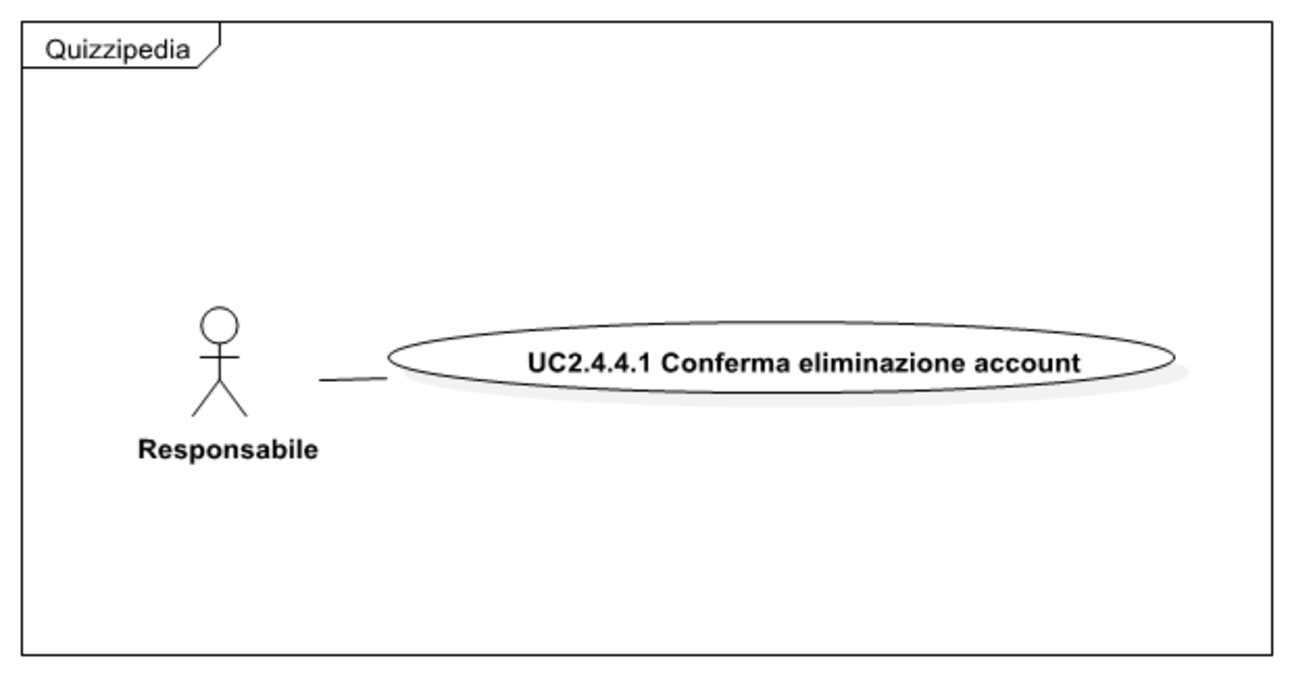
\includegraphics[width=\textwidth]{Img/UC Eliminazione account.pdf}}
\caption{UC2.4.4 Eliminazione account}
\end{figure}
\begin{itemize}
\item \textbf{Attori}: Responsabile.
\item \textbf{Scenario principale}:
\begin{enumerate}
\item Conferma eliminazione account (UC2.4.4.1).
\end{enumerate}
\item \textbf{Descrizione}: il responsabile può rimuovere dal proprio ente gli utenti che gestisce.
\item \textbf{Precondizione}: il responsabile è autenticato.
\item \textbf{Postcondizione}: il responsabile ha selezionato l'account da rimuovere.
\end{itemize}
\subsubsection{UC2.4.4.1 Conferma eliminazione account}
\begin{itemize}
\item \textbf{Attori}: Responsabile.
\item \textbf{Scenario principale}: il responsabile conferma l'eliminazione dell'account.
\item \textbf{Descrizione}: Il responsabile deve confermare la rimozione dell'utente.
\item \textbf{Precondizione}: Il responsabile si trova nella pagina di eliminazione di altri account.
\item \textbf{Postcondizione}: Il responsabile ha confermato la rimozione  dell'utente.
\end{itemize}
\subsubsection{UC2.4.5 Interruzione volontaria della modifica delle informazioni personali}
\begin{itemize}
\item \textbf{Attori}: Utente Autenticato.
\item \textbf{Scenario principale}: l'utente interrompe la modifica delle informazioni personali.
\item \textbf{Descrizione}: l'utente può interrompere la modifica delle informazioni personali.
\item \textbf{Precondizione}: l'utente sta modificando le proprie informazioni personali.
\item \textbf{Postcondizione}: l'utente non ha completato la modifica delle informazioni personali.
\end{itemize}
\subsubsection{UC2.5 Richiesta accettazione}
\begin{figure}[H]
\centering
\noindent\makebox[\textwidth]{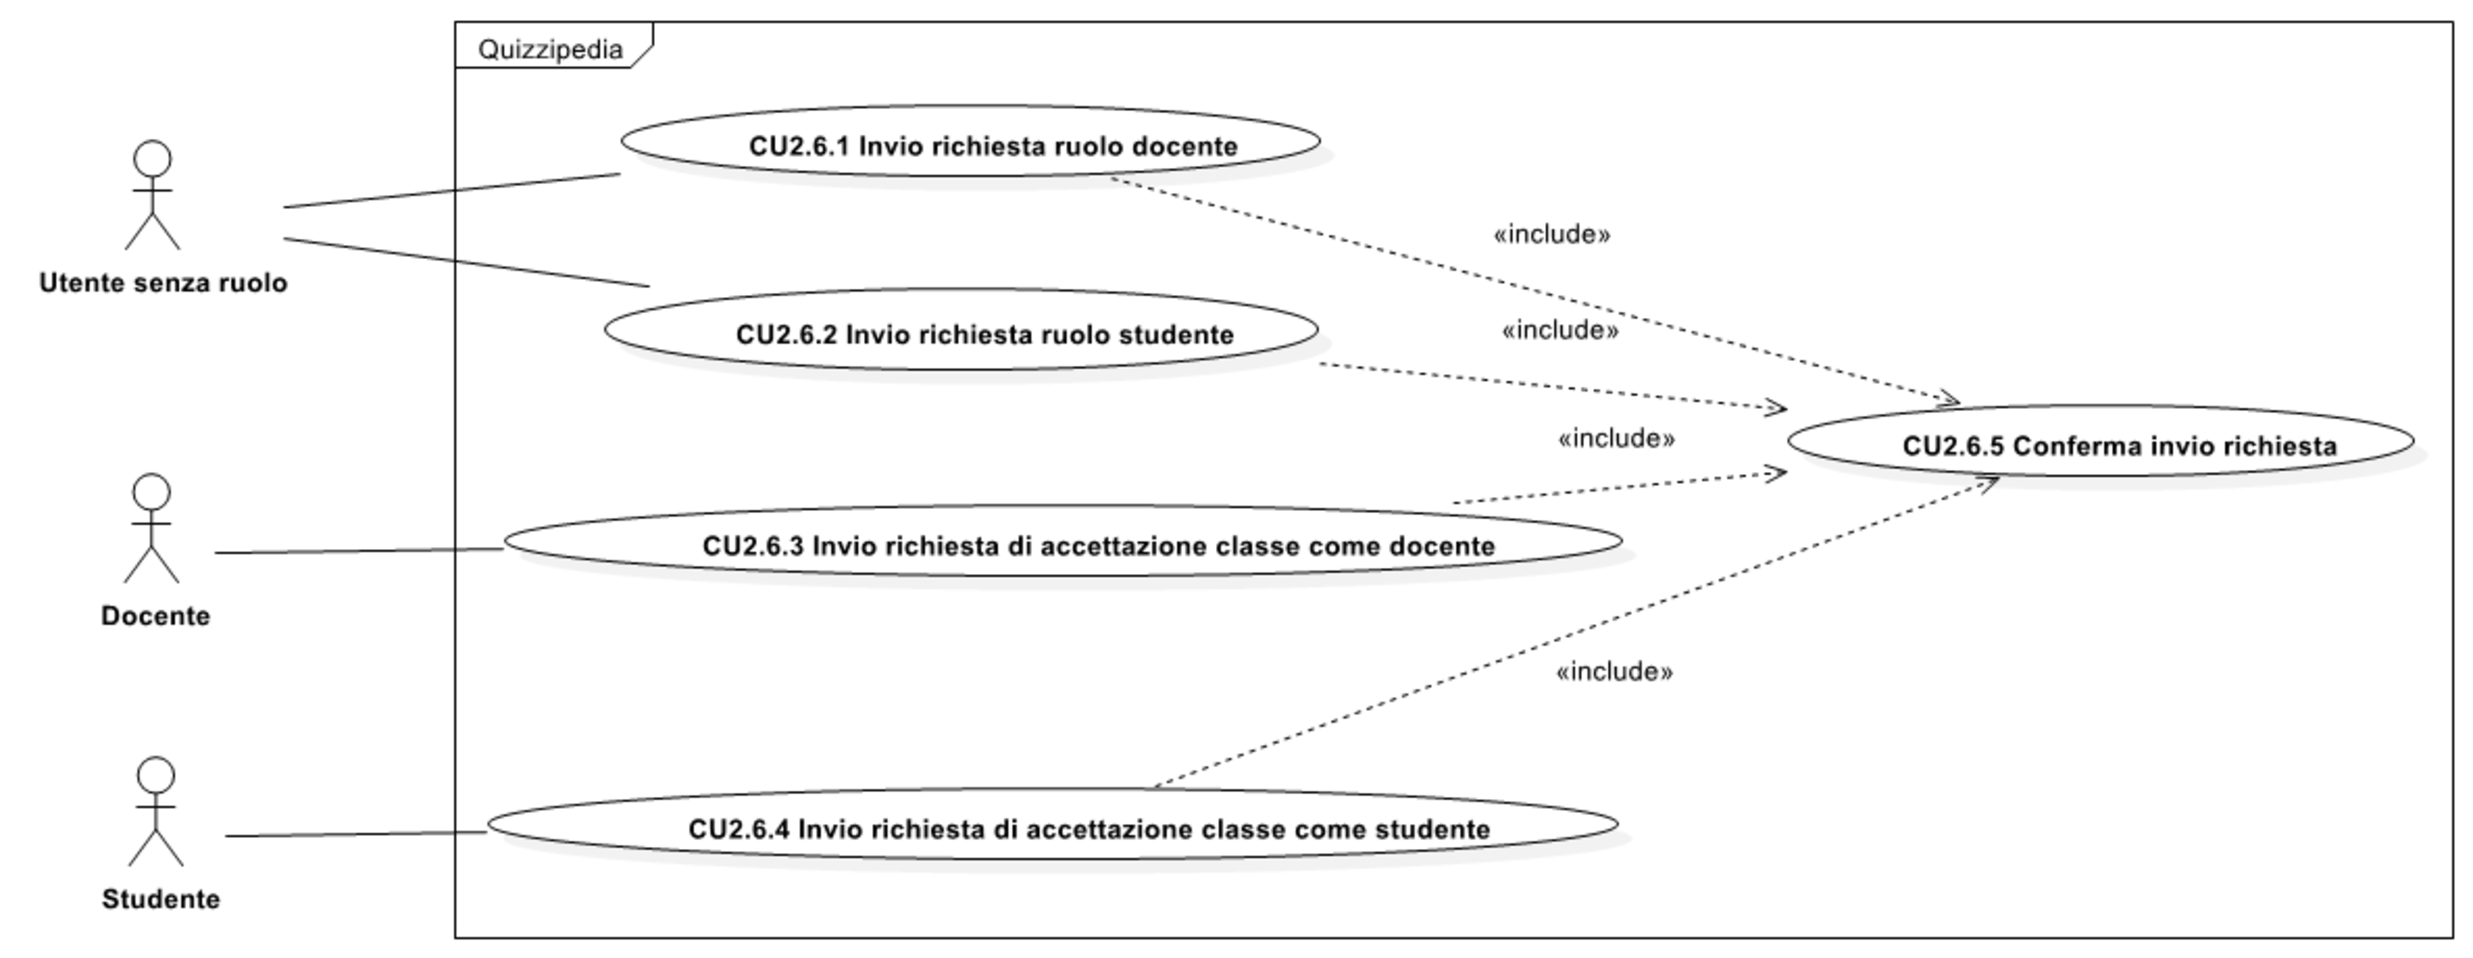
\includegraphics[width=\textwidth]{Img/UC Richiesta accettazione.pdf}}
\caption{UC2.5 Richiesta accettazione}
\end{figure}
\begin{itemize}
\item \textbf{Attori}: Docente, Studente, Utente senza Ruolo.
\item \textbf{Scenario principale}:
\begin{enumerate}
\item Invio richiesta ruolo docente (UC2.5.1);
\item Invio richiesta ruolo studente (UC2.5.2);
\item Invio richiesta di accettazione classe come docente (UC2.5.3);
\item Invio richiesta di accettazione classe come studente (UC2.5.4).
\end{enumerate}
\item \textbf{Descrizione}: l’utente senza ruolo invia una richiesta per essere studente o docente, mentre studente e docente inviano una richiesta di accettazione per essere inseriti in una determinata classe.
\item \textbf{Precondizione}: utente senza ruolo, studente e docente possono inviare richieste di accettazione.
\item \textbf{Postcondizione}: è stata inviata una richesta d’accettazione e sarà notificata al responsabile.
\end{itemize}
\subsubsection{UC2.5.1 Invio richiesta ruolo docente}
\begin{itemize}
\item \textbf{Attori}: Utente senza Ruolo.
\item \textbf{Scenario principale}: l'utente invia la richiesta di ruolo 'docente'.
\item \textbf{Descrizione}: l'utente senza ruolo compila la richiesta per acquisire il ruolo di docente che sarà successivamente accettata  o rifiutata dal responsabile.
\item \textbf{Precondizione}: l'utente deve essere un utente senza ruolo.
\item \textbf{Postcondizione}: l'utente senza ruolo ha compilato la richiesta di acquisizione ruolo docente.
\end{itemize}
\subsubsection{UC2.5.2 Invio richiesta ruolo studente}
\begin{itemize}
\item \textbf{Attori}: Utente senza Ruolo.
\item \textbf{Scenario principale}: l'utente invia la richiesta di ruolo 'studente'.
\item \textbf{Descrizione}: l'utente senza ruolo compila la richiesta per acquisire il ruolo di studente che sarà successivamente accettata o rifiutata dal responsabile.
\item \textbf{Precondizione}: l'utente deve essere un utente senza ruolo.
\item \textbf{Postcondizione}: l'utente senza ruolo ha compilato la richiesta di acquisizione ruolo studente.
\end{itemize}
\subsubsection{UC2.5.3 Invio richiesta di accettazione classe come docente}
\begin{figure}[H]
\centering
\noindent\makebox[\textwidth]{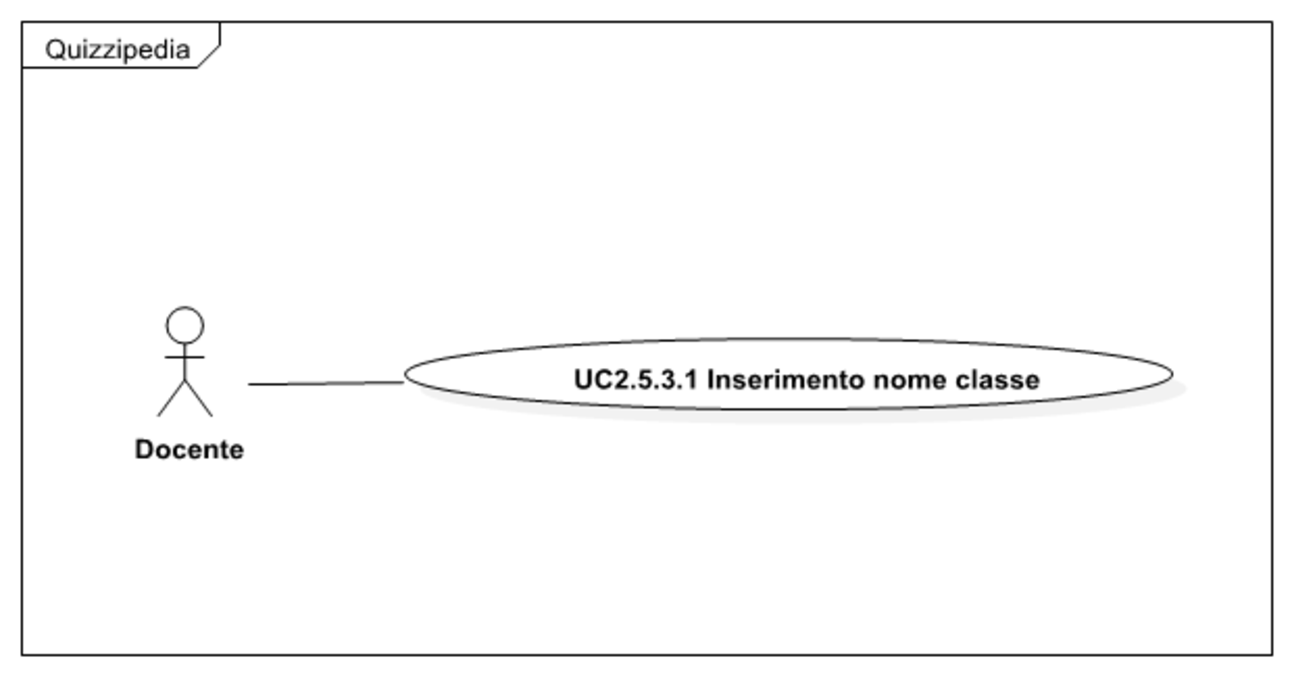
\includegraphics[width=\textwidth]{Img/UC Invio richiesta di accettazione classe come docente.pdf}}
\caption{UC2.5.3 Invio richiesta di accettazione classe come docente}
\end{figure}
\begin{itemize}
\item \textbf{Attori}: Docente.
\item \textbf{Scenario principale}:
\begin{enumerate}
\item Inserimento nome classe (UC2.5.3.1).
\end{enumerate}
\item \textbf{Descrizione}: il docente invia una richiesta al responsabile con il nome della classe per avere il permesso di essere inserito nella classe indicata.
\item \textbf{Precondizione}: il docente ha il permesso di inviare la richiesta.
\item \textbf{Postcondizione}: il docente ha compilato la richiesta.
\end{itemize}
\subsubsection{UC2.5.3.1 Inserimento nome classe}
\begin{itemize}
\item \textbf{Attori}: Docente.
\item \textbf{Scenario principale}: il docente seleziona il nome della classe.
\item \textbf{Descrizione}: il docente deve poter selezionare il nome della classe alla quale vuole essere inserito.
\item \textbf{Precondizione}: il docente è nella fase di invio richiesta di accettazione classe come docente.
\item \textbf{Postcondizione}: il docente ha selezionato il nome della classe.
\end{itemize}
\subsubsection{UC2.5.4 Invio richiesta di accettazione classe come studente}
\begin{figure}[H]
\centering
\noindent\makebox[\textwidth]{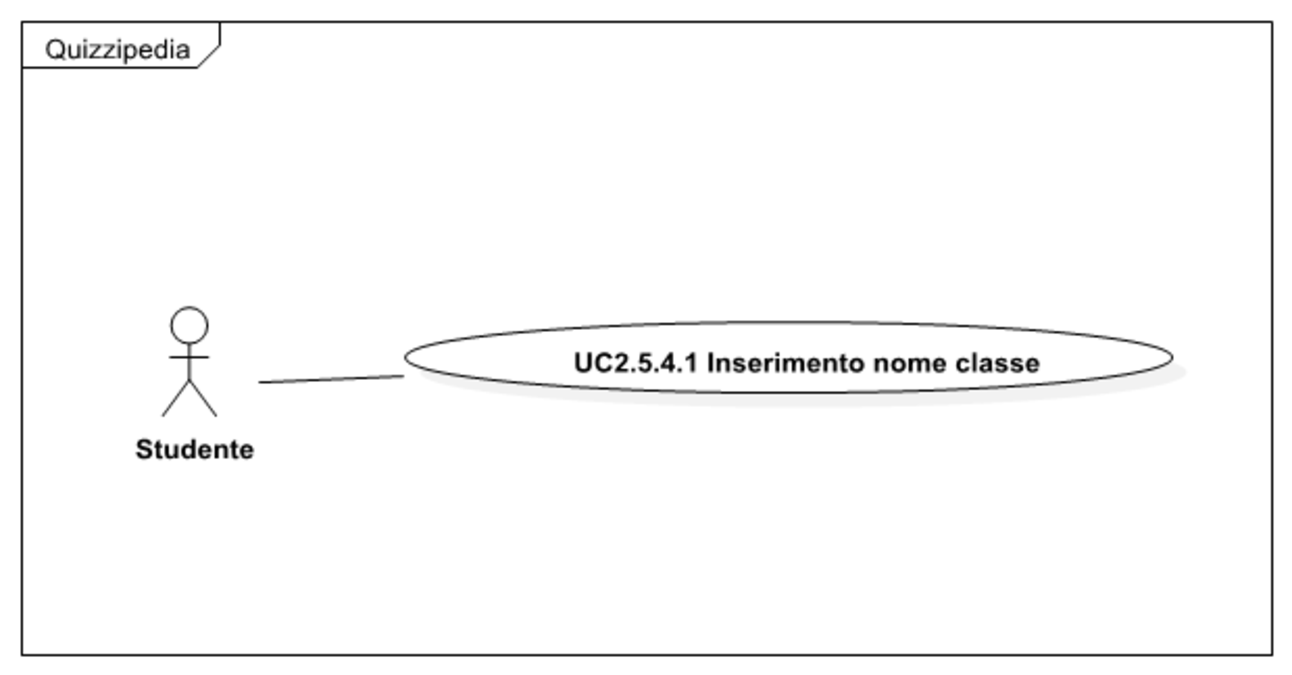
\includegraphics[width=\textwidth]{Img/UC Invio richiesta di accettazione classe come studente.pdf}}
\caption{UC2.5.4 Invio richiesta di accettazione classe come studente}
\end{figure}
\begin{itemize}
\item \textbf{Attori}: Studente.
\item \textbf{Scenario principale}:
\begin{enumerate}
\item Inserimento nome classe (UC2.5.4.1).
\end{enumerate}
\item \textbf{Descrizione}: lo studente invia una richiesta al responsabile con il nome della classe per avere il permesso di essere inserito nella classe indicata.
\item \textbf{Precondizione}: lo studente ha il permesso di inviare questa richiesta.
\item \textbf{Postcondizione}: lo studente ha compilato la richiesta.
\end{itemize}
\subsubsection{UC2.5.4.1 Inserimento nome classe}
\begin{itemize}
\item \textbf{Attori}: Studente.
\item \textbf{Scenario principale}: l'utente seleziona il nome della classe.
\item \textbf{Descrizione}: lo studente deve poter selezionare il nome della classe alla quale vuole essere inserito.
\item \textbf{Precondizione}: lo studente è nella fase di invio di richiesta di accettazione classe come studente.
\item \textbf{Postcondizione}: lo studente ha selezionato il nome della classe.
\end{itemize}
\subsubsection{UC2.6 Visualizzazione statistiche}
\begin{figure}[H]
\centering
\noindent\makebox[\textwidth]{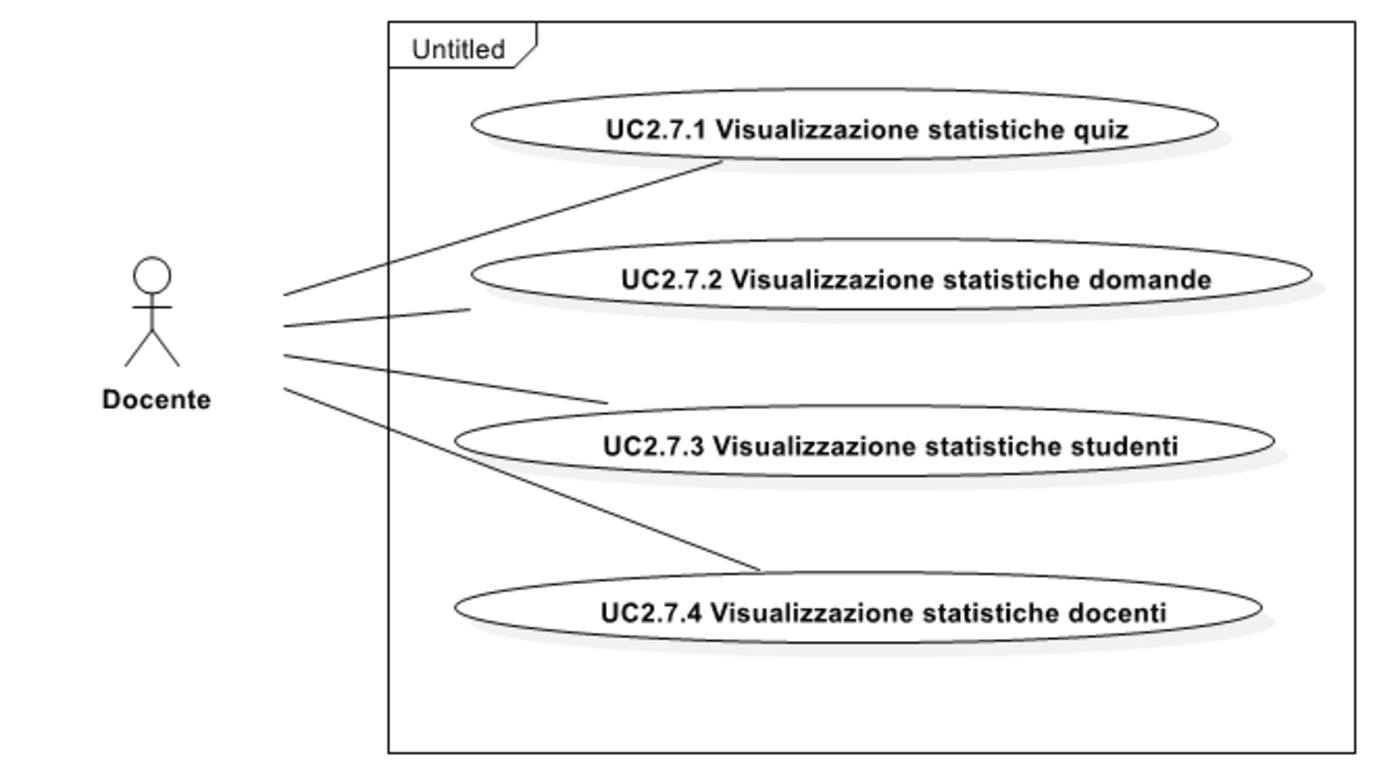
\includegraphics[width=\textwidth]{Img/UC Visualizzazione statistiche.pdf}}
\caption{UC2.6 Visualizzazione statistiche}
\end{figure}
\begin{itemize}
\item \textbf{Attori}: Docente.
\item \textbf{Scenario principale}:
\begin{enumerate}
\item Visualizzazione statistiche quiz (UC2.6.1);
\item Visualizzazione statistiche domande (UC2.6.2);
\item Visualizzazione statistiche studenti (UC2.6.3);
\item Visualizzazione statistiche docenti (UC2.6.4).
\end{enumerate}
\item \textbf{Descrizione}: il docente deve poter visualizzare statistiche di vario tipo relative a quiz, domande, studenti e altri docenti.
\item \textbf{Precondizione}: il docente è autenticato nel sistema e desidera visualizzare le statistiche.
\item \textbf{Postcondizione}: il docente ha visualizzato le statistiche.
\end{itemize}
\subsubsection{UC2.6.1 Visualizzazione statistiche quiz}
\begin{figure}[H]
\centering
\noindent\makebox[\textwidth]{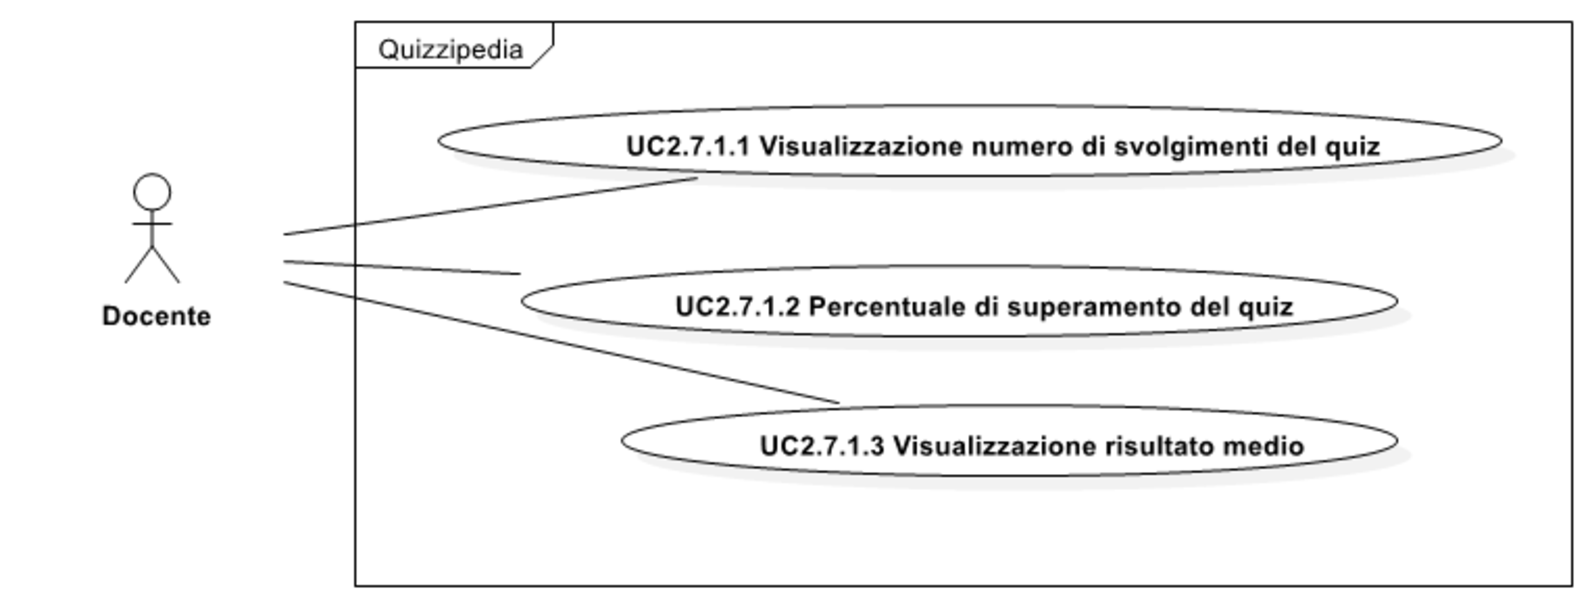
\includegraphics[width=\textwidth]{Img/UC Visualizzazione statistiche quiz.pdf}}
\caption{UC2.6.1 Visualizzazione statistiche quiz}
\end{figure}
\begin{itemize}
\item \textbf{Attori}: Docente.
\item \textbf{Scenario principale}:
\begin{enumerate}
\item Visualizzazione numero di svolgimenti (UC2.6.1.1);
\item Visualizzazione percentuale di superamento del quiz (UC2.6.1.2);
\item Visualizzazione risultato medio (UC2.6.1.3).
\end{enumerate}
\item \textbf{Descrizione}: il docente deve poter visualizzare statistiche legate ai quiz.
\item \textbf{Precondizione}: il docente è autenticato nel sistema e desidera visualizzare le statistiche legate ai quiz.
\item \textbf{Postcondizione}: il docente ha visualizzato le statistiche legate ai quiz.
\end{itemize}
\subsubsection{UC2.6.1.1 Visualizzazione numero di svolgimenti}
\begin{itemize}
\item \textbf{Attori}: Docente.
\item \textbf{Scenario principale}: il docente visualizza il numero di volte in cui un quiz è stato svolto.
\item \textbf{Descrizione}: il docente deve poter visualizzare il numero di volte in cui un quiz è stato svolto.
\item \textbf{Precondizione}: il docente ha deciso di visualizzare le statistiche legate ai quiz.
\item \textbf{Postcondizione}: il docente ha visualizzato il numero di svolgimenti di un quiz.
\end{itemize}
\subsubsection{UC2.6.1.2 Visualizzazione percentuale di superamento del quiz}
\begin{itemize}
\item \textbf{Attori}: Docente.
\item \textbf{Scenario principale}: il docente visualizza la percentuale di studenti che hanno svolto il quiz con esito positivo.
\item \textbf{Descrizione}: il docente deve poter visualizzare la percentuale di studenti che hanno svolto il quiz con esito positivo.
\item \textbf{Precondizione}: il docente ha deciso di visualizzare le statistiche legate ai quiz.
\item \textbf{Postcondizione}: il docente ha visualizzato la percentuale di superamento di un quiz.
\end{itemize}
\subsubsection{UC2.6.1.3 Visualizzazione risultato medio}
\begin{itemize}
\item \textbf{Attori}: Docente.
\item \textbf{Scenario principale}: il docente visualizza il risultato medio ottenuto dagli utenti che hanno svolto il quiz.
\item \textbf{Descrizione}: il docente deve poter visualizzare il risultato medio ottenuto dagli utenti che hanno svolto il quiz.
\item \textbf{Precondizione}: il docente ha deciso di visualizzare le statistiche legate ai quiz.
\item \textbf{Postcondizione}: il docente ha visualizzato il risultato medio di un quiz.
\end{itemize}
\subsubsection{UC2.6.2 Visualizzazione statistiche domande}
\begin{figure}[H]
\centering
\noindent\makebox[\textwidth]{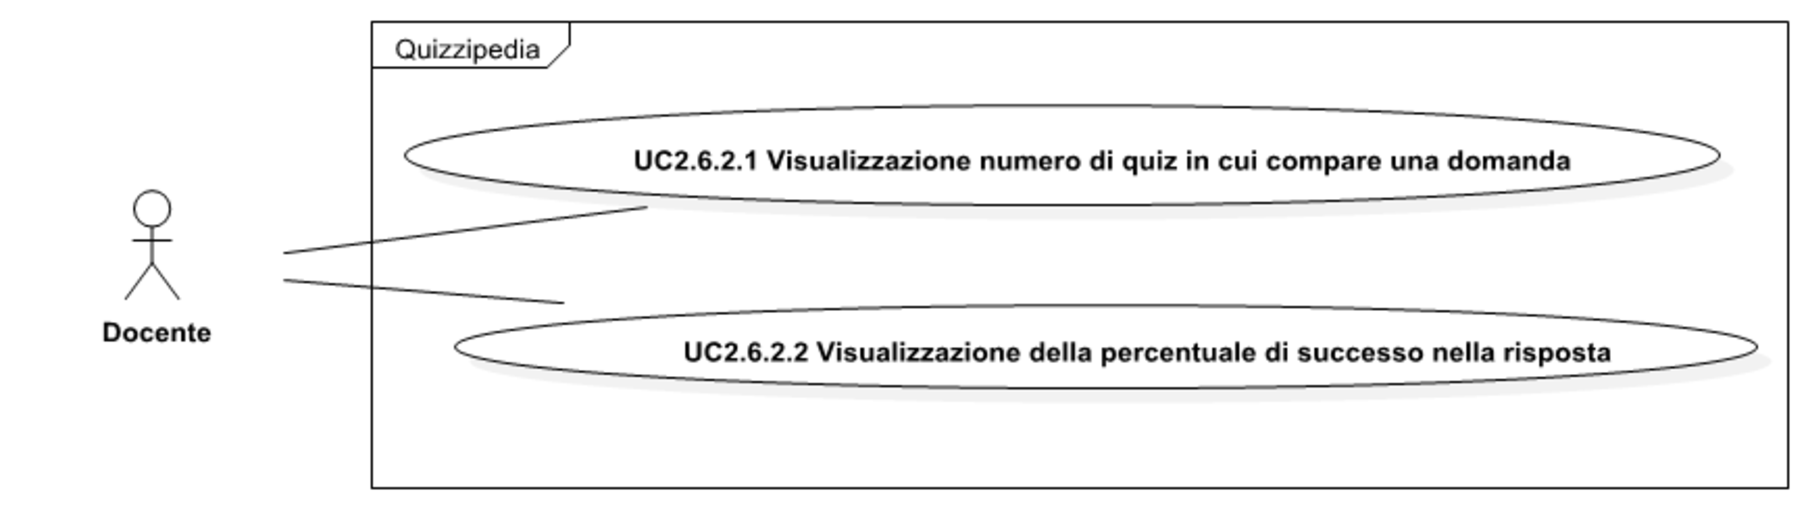
\includegraphics[width=\textwidth]{Img/UC Visualizzazione statistiche domande.pdf}}
\caption{UC2.6.2 Visualizzazione statistiche domande}
\end{figure}
\begin{itemize}
\item \textbf{Attori}: Docente.
\item \textbf{Scenario principale}:
\begin{enumerate}
\item Visualizzazione numero di quiz in cui compare una domanda (UC2.6.2.1);
\item Visualizzazione percentuale di successo nella risposta (UC2.6.2.2).
\end{enumerate}
\item \textbf{Descrizione}: il docente deve poter visualizzare statistiche legate alle domande.
\item \textbf{Precondizione}: il docente è autenticato nel sistema e desidera visualizzare le statistiche legate alle domande.
\item \textbf{Postcondizione}: il docente ha visualizzato le statistiche legate alle domande.
\end{itemize}
\subsubsection{UC2.6.2.1 Visualizzazione numero di quiz in cui compare una domanda}
\begin{itemize}
\item \textbf{Attori}: Docente.
\item \textbf{Scenario principale}: il docente visualizza il numero di quiz in cui compare la domanda.
\item \textbf{Descrizione}: il docente deve poter visualizzare il numero di quiz in cui compare la domanda.
\item \textbf{Precondizione}: il docente ha deciso di visualizzare le statistiche legate alle domande.
\item \textbf{Postcondizione}: il docente ha visualizzato il numero di quiz in cui compare una domanda.
\end{itemize}
\subsubsection{UC2.6.2.2 Visualizzazione percentuale di successo nella risposta}
\begin{itemize}
\item \textbf{Attori}: Docente.
\item \textbf{Scenario principale}: il docente visualizza la percentuale di successo nella risposta della domanda.
\item \textbf{Descrizione}: il docente deve poter visualizzare la percentuale di successo nella risposta della domanda.
\item \textbf{Precondizione}: il docente ha deciso di visualizzare le statistiche legate alle domande.
\item \textbf{Postcondizione}: il docente ha visualizzato la percentuale di successo nella risposta a una domanda.
\end{itemize}
\subsubsection{UC2.6.3 Visualizzazione statistiche studenti}
\begin{figure}[H]
\centering
\noindent\makebox[\textwidth]{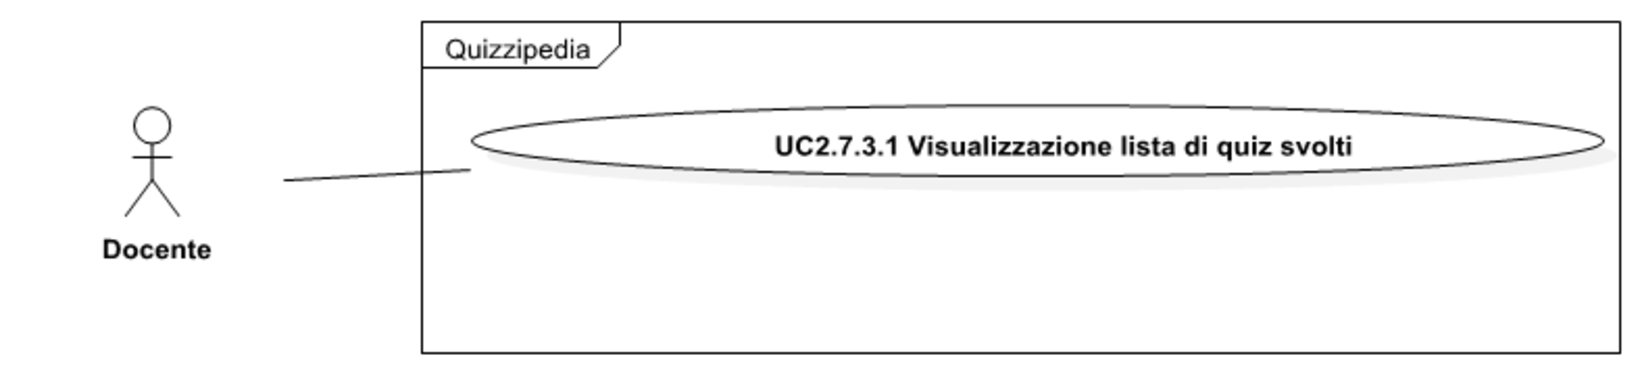
\includegraphics[width=\textwidth]{Img/UC Visualizzazione statistiche studenti.pdf}}
\caption{UC2.6.3 Visualizzazione statistiche studenti}
\end{figure}
\begin{itemize}
\item \textbf{Attori}: Docente.
\item \textbf{Scenario principale}:
\begin{enumerate}
\item Visualizzazione lista di quiz svolti (UC2.6.3.1).
\end{enumerate}
\item \textbf{Descrizione}:  il docente deve poter visualizzare statistiche legate agli studenti.
\item \textbf{Precondizione}: il docente è autenticato nel sistema e desidera visualizzare le statistiche legate agli studenti.
\item \textbf{Postcondizione}: il docente ha visualizzato le statistiche legate agli studenti.
\end{itemize}
\subsubsection{UC2.6.3.1 Visualizzazione lista di quiz svolti}
\begin{itemize}
\item \textbf{Attori}: Docente.
\item \textbf{Scenario principale}: il docente visualizza una lista dei quiz svolti dallo studente con rispettivo risultato.
\item \textbf{Descrizione}: il docente deve poter visualizzare una lista dei quiz svolti dallo studente con rispettivo risultato.
\item \textbf{Precondizione}: il docente ha deciso di visualizzare le statistiche legate agli studenti.
\item \textbf{Postcondizione}: il docente ha visualizzato la lista dei quiz svolti da uno studente.
\end{itemize}
\subsubsection{UC2.6.4 Visualizzazione statistiche docenti}
\begin{figure}[H]
\centering
\noindent\makebox[\textwidth]{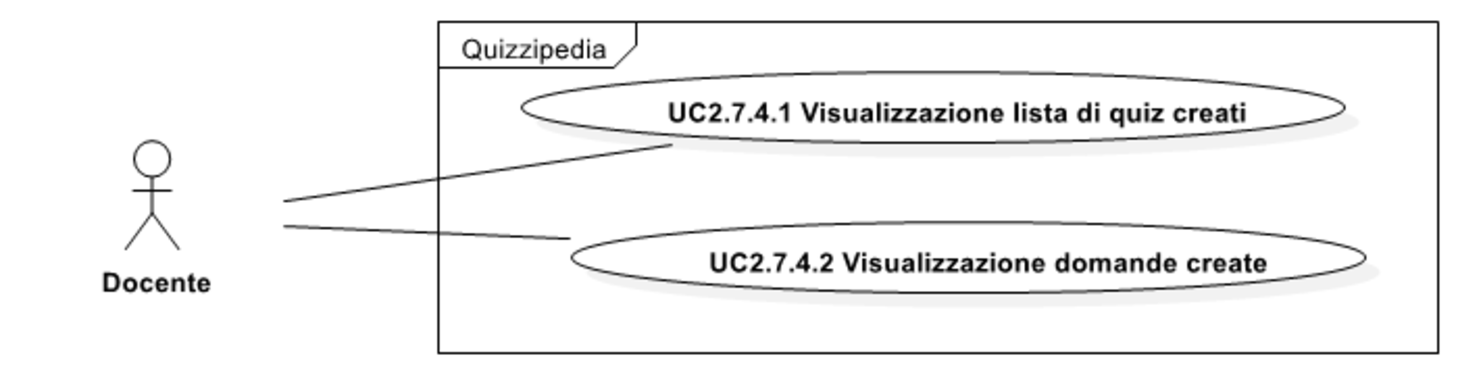
\includegraphics[width=\textwidth]{Img/UC Visualizzazione statistiche docenti.pdf}}
\caption{UC2.6.4 Visualizzazione statistiche docenti}
\end{figure}
\begin{itemize}
\item \textbf{Attori}: Docente.
\item \textbf{Scenario principale}:
\begin{enumerate}
\item Visualizzazione lista di quiz creati (UC2.6.4.1);
\item Visualizzazione lista di domande create (UC2.6.4.2).
\end{enumerate}
\item \textbf{Descrizione}: il docente deve poter visualizzare statistiche legate ai docenti.
\item \textbf{Precondizione}: il docente è autenticato nel sistema e desidera visualizzare le statistiche legate ai docenti.
\item \textbf{Postcondizione}: il docente ha visualizzato le statistiche legate ai docenti.
\end{itemize}
\subsubsection{UC2.6.4.1 Visualizzazione lista di quiz creati}
\begin{itemize}
\item \textbf{Attori}: Docente.
\item \textbf{Scenario principale}: il docente visualizza una lista dei quiz creati dal docente.
\item \textbf{Descrizione}: il docente deve poter visualizzare una lista dei quiz creati dal docente.
\item \textbf{Precondizione}: il docente ha deciso di visualizzare le statistiche legate ai docenti.
\item \textbf{Postcondizione}: il docente ha visualizzato la lista dei quiz creati da un docente.
\end{itemize}
\subsubsection{UC2.6.4.2 Visualizzazione lista di domande create}
\begin{itemize}
\item \textbf{Attori}: Docente.
\item \textbf{Scenario principale}: il docente visualizza una lista delle domande create dal docente.
\item \textbf{Descrizione}: il docente deve poter visualizzare una lista delle domande create dal docente.
\item \textbf{Precondizione}: il docente ha deciso di visualizzare le statistiche legate ai docenti.
\item \textbf{Postcondizione}: il docente ha visualizzato la lista delle domande create da un docente.
\end{itemize}
\subsubsection{UC2.7 Modifica ente}
\begin{figure}[H]
\centering
\noindent\makebox[\textwidth]{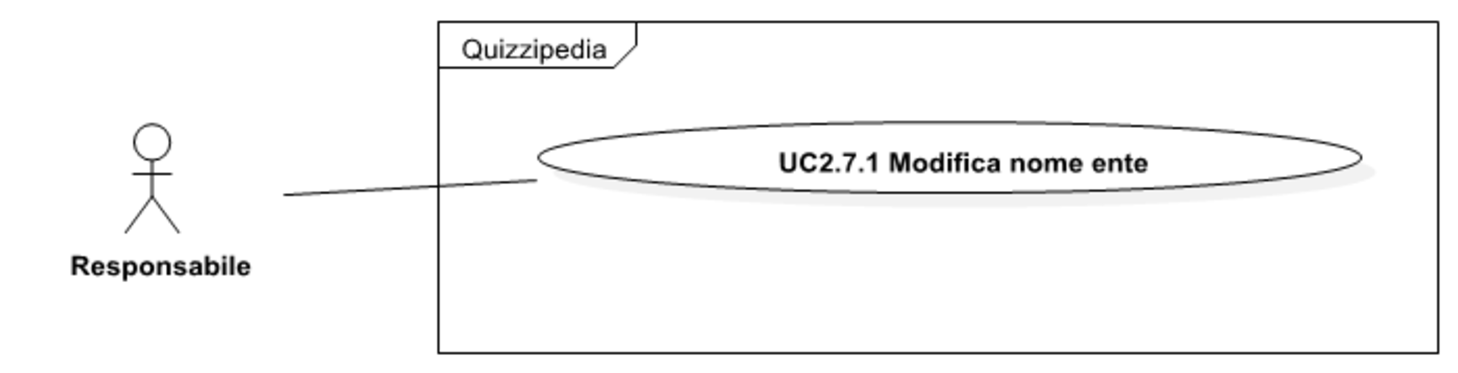
\includegraphics[width=\textwidth]{Img/UC Modifica ente.pdf}}
\caption{UC2.7 Modifica ente}
\end{figure}
\begin{itemize}
\item \textbf{Attori}: Responsabile.
\item \textbf{Scenario principale}:
\begin{enumerate}
\item Modifica nome ente (UC2.7.1).
\end{enumerate}
\item \textbf{Descrizione}: il responsabile deve poter modificare l'ente di cui è a capo.
\item \textbf{Precondizione}: il responsabile ha il permesso di modificare l'ente.
\item \textbf{Postcondizione}: il responsabile ha completato la modifica delle informazioni desiderate riguardanti l'ente.
\end{itemize}
\subsubsection{UC2.7.1 Modifica nome ente}
\begin{figure}[H]
\centering
\noindent\makebox[\textwidth]{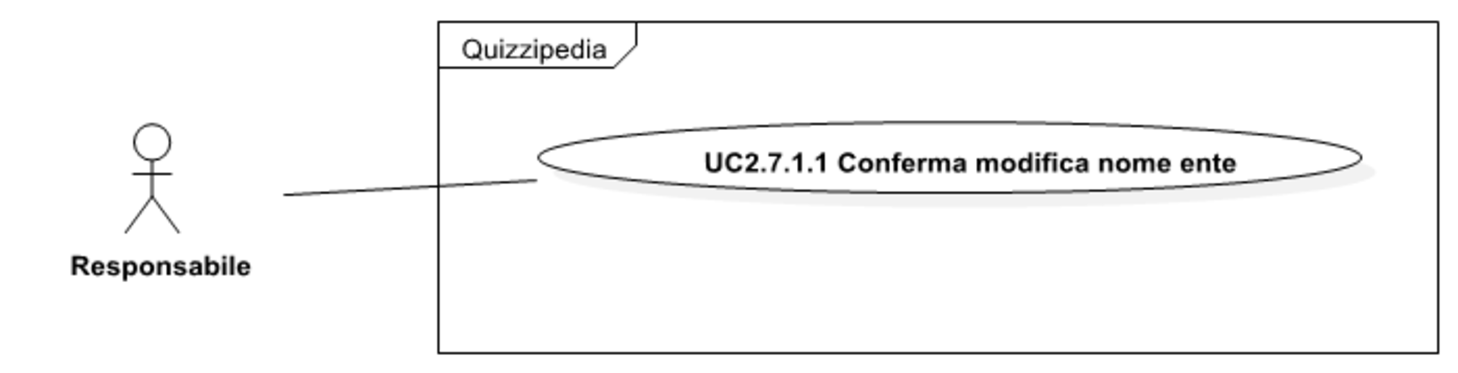
\includegraphics[width=\textwidth]{Img/UC Modifica nome ente.pdf}}
\caption{UC2.7.1 Modifica nome ente}
\end{figure}
\begin{itemize}
\item \textbf{Attori}: Responsabile.
\item \textbf{Scenario principale}:
\begin{enumerate}
\item Conferma modifica nome ente (UC2.7.1.1).
\end{enumerate}
\item \textbf{Descrizione}: il responsabile deve poter modificare il nome dell'ente che ha precedentemente creato.
\item \textbf{Precondizione}: il responsabile ha il permesso di modificare il nome dell'ente.
\item \textbf{Postcondizione}: il responsabile ha modificato il nome dell'ente.
\end{itemize}
\subsubsection{UC2.7.1.1 Conferma modifica nome ente}
\begin{itemize}
\item \textbf{Attori}: Responsabile.
\item \textbf{Scenario principale}: il responsabile conferma la modifica del nome dell'ente.
\item \textbf{Descrizione}: il responsabile deve confermare la modifica del nome dell'ente.
\item \textbf{Precondizione}: il responsabile sta modificando i dati dell'ente e deve confermarne il nome.
\item \textbf{Postcondizione}: il responsabile ha confermato la modifica del nome dell'ente.
\end{itemize}
\subsubsection{UC2.8 Gestione classi}
\begin{figure}[H]
\centering
\noindent\makebox[\textwidth]{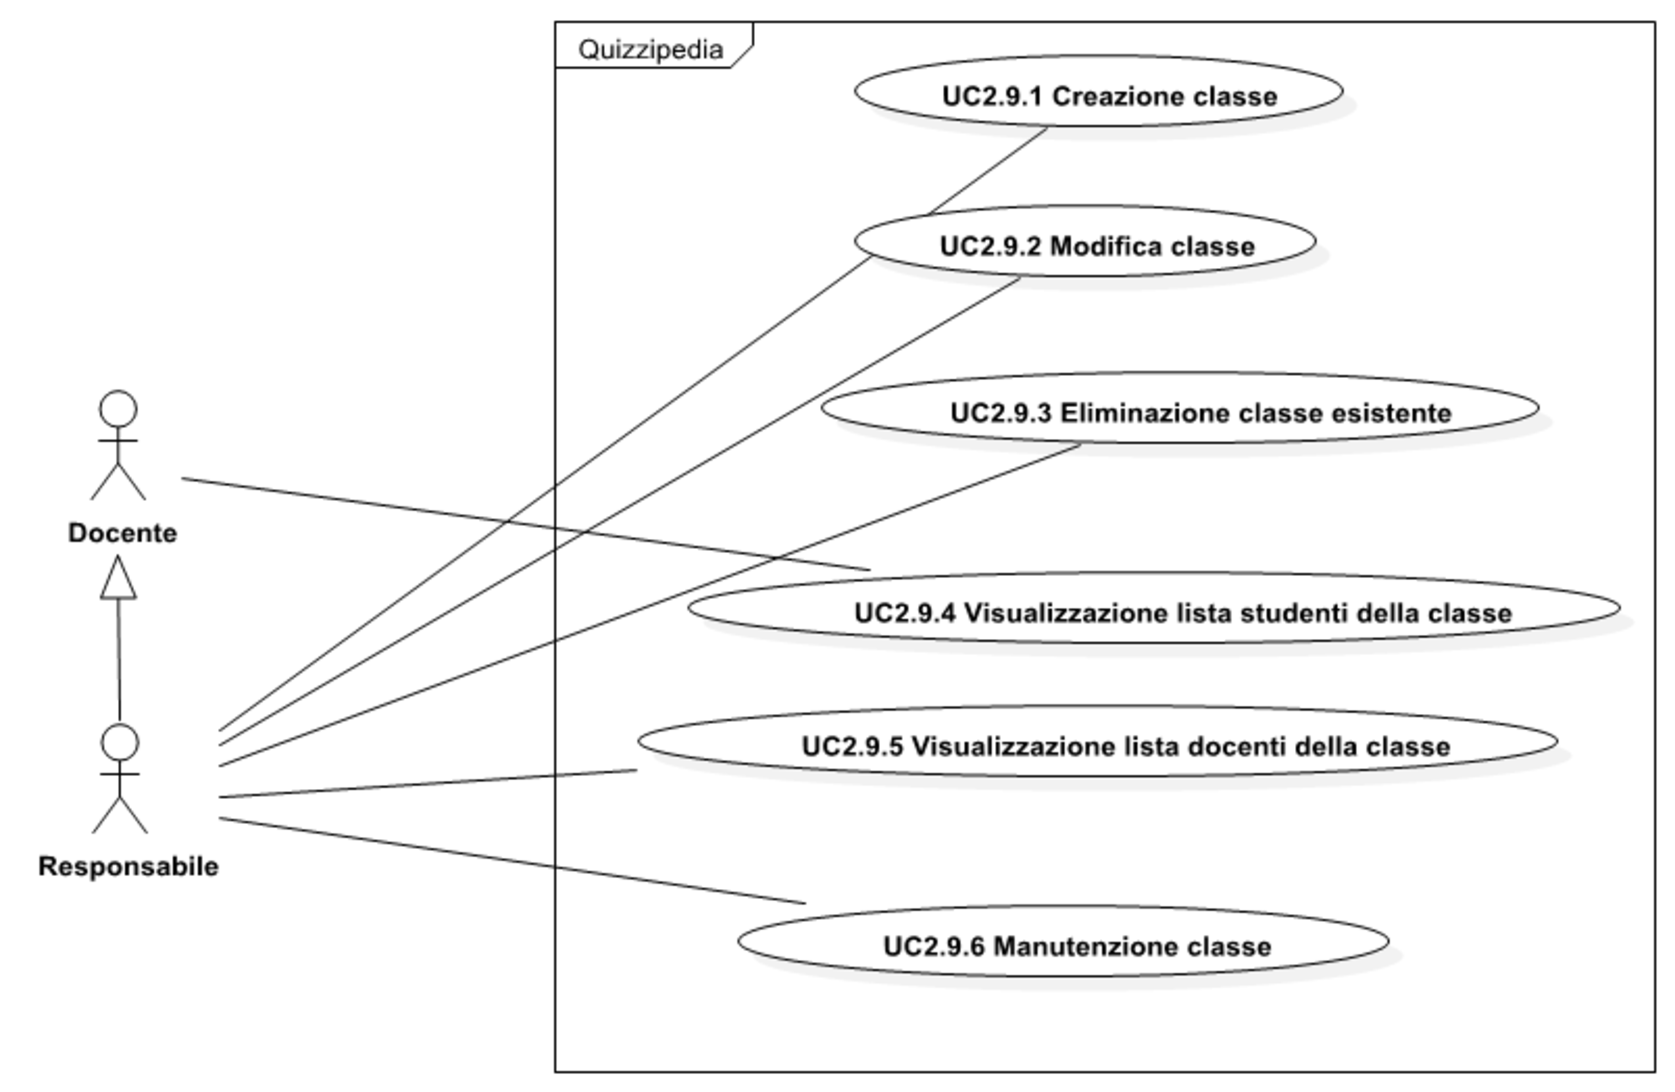
\includegraphics[width=\textwidth]{Img/UC Gestione classi.pdf}}
\caption{UC2.8 Gestione classi}
\end{figure}
\begin{itemize}
\item \textbf{Attori}: Responsabile.
\item \textbf{Scenario principale}:
\begin{enumerate}
\item Creazione classe (UC2.8.1);
\item Modifica classe (UC2.8.2);
\item Eliminazione classe (UC2.8.3);
\item Visualizza lista studenti della classe (UC2.8.4);
\item Visualizza lista docenti della classe (UC2.8.5);
\item Manutenzione classe (UC2.8.6).
\end{enumerate}
\item \textbf{Descrizione}: il responsabile può creare, modificare ed eliminare una classe; inoltre può visualizzare la lista degli studenti e docenti della classe; può fare manutenzione sulle classi nel caso in cui le richieste di inserimento da parte di studenti e docenti siano sbagliate; infine gestisce la lista delle richieste che riceve da parte degli studenti e docenti.
\item \textbf{Precondizione}: il responsabile ha i permessi per gestire le classi.
\item \textbf{Postcondizione}: il responsabile ha effettuato le operazioni di gestione delle classi.
\end{itemize}
\subsubsection{UC2.8.1 Creazione classe}
\begin{figure}[H]
\centering
\noindent\makebox[\textwidth]{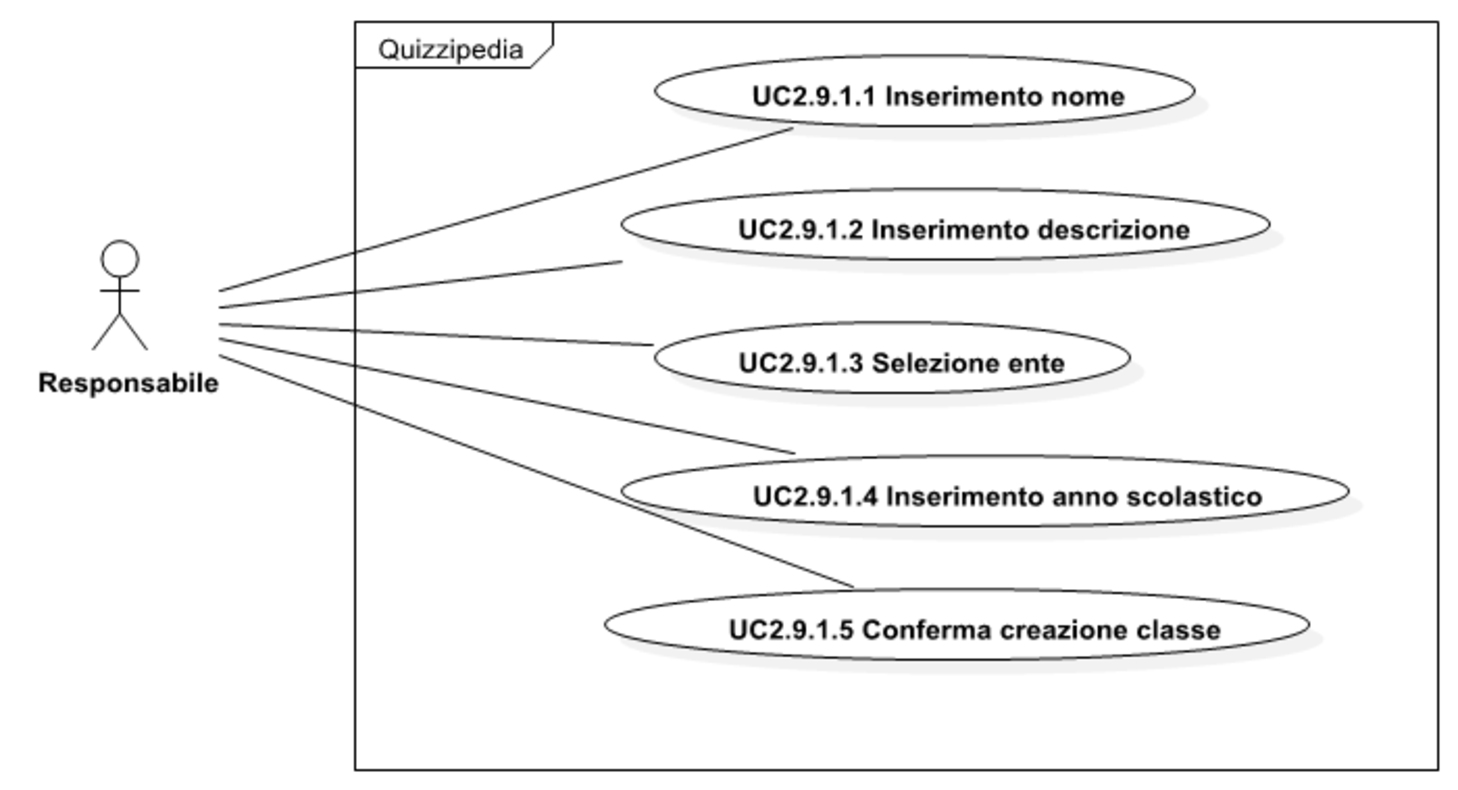
\includegraphics[width=\textwidth]{Img/UC Creazione classe.pdf}}
\caption{UC2.8.1 Creazione classe}
\end{figure}
\begin{itemize}
\item \textbf{Attori}: Responsabile.
\item \textbf{Scenario principale}:
\begin{enumerate}
\item Inserimento nome (UC2.8.1.1);
\item Inserimento descrizione (UC2.8.1.2);
\item Inserimento anno scolastico (UC2.8.1.3);
\item Conferma creazione classe (UC2.8.1.4).
\end{enumerate}
\item \textbf{Descrizione}: il responsabile deve poter creare una classe.
\item \textbf{Precondizione}: il responsabile ha i permessi per creare una classe ed è nella gestione classe.
\item \textbf{Postcondizione}: il responsabile ha creato una nuova classe.
\end{itemize}
\subsubsection{UC2.8.1.1 Inserimento nome}
\begin{itemize}
\item \textbf{Attori}: Responsabile.
\item \textbf{Scenario principale}: il responsabile inserisce il nome della classe.
\item \textbf{Descrizione}: il responsabile deve poter inserire il nome della classe.
\item \textbf{Precondizione}: il responsabile sta creando una classe e deve ancora inserire il nome.
\item \textbf{Postcondizione}: il responsabile ha inserito il nome della classe.
\end{itemize}
\subsubsection{UC2.8.1.2 Inserimento descrizione}
\begin{itemize}
\item \textbf{Attori}: Responsabile.
\item \textbf{Scenario principale}: il responsabile inserisce la descrizione della classe.
\item \textbf{Descrizione}: il responsabile può inserire una breve descrizione della classe.
\item \textbf{Precondizione}: il responsabile sta creando una classe e deve ancora inserire la descrizione.
\item \textbf{Postcondizione}: il responsabile ha inserito una breve descrizione della classe.
\end{itemize}
\subsubsection{UC2.8.1.3 Inserimento anno scolastico}
\begin{itemize}
\item \textbf{Attori}: Responsabile.
\item \textbf{Scenario principale}: il responsabile inserisce l'anno scolastico di creazione della classe.
\item \textbf{Descrizione}: il responsabile deve inserire l'anno scolastico in cui è stata creata la classe.
\item \textbf{Precondizione}: il responsabile sta creando una classe e deve ancora inserire l'anno scolastico.
\item \textbf{Postcondizione}: il responsabile ha inserito l'anno scolastico della classe.
\end{itemize}
\subsubsection{UC2.8.1.4 Conferma creazione classe}
\begin{itemize}
\item \textbf{Attori}: Responsabile.
\item \textbf{Scenario principale}: il responsabile conferma i dati per la creazione della classe.
\item \textbf{Descrizione}: il responsabile deve confermare i dati precedentemente inseriti.
\item \textbf{Precondizione}: il responsabile ha inserito una nuova classe e deve ancora confermarla.
\item \textbf{Postcondizione}: il responsabile ha confermato i dati inseriti e la classe è stata creata.
\end{itemize}
\subsubsection{UC2.8.2 Modifica classe}
\begin{figure}[H]
\centering
\noindent\makebox[\textwidth]{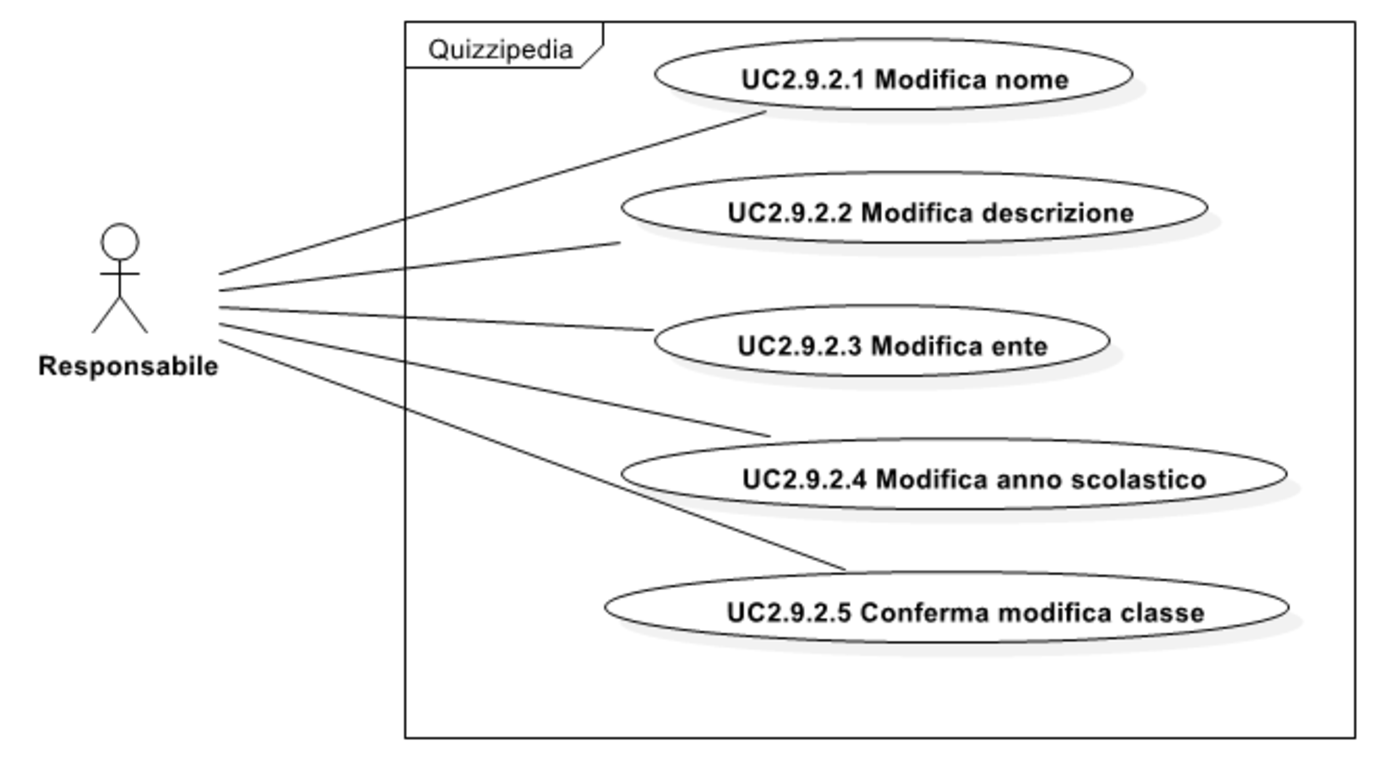
\includegraphics[width=\textwidth]{Img/UC Modifica classe.pdf}}
\caption{UC2.8.2 Modifica classe}
\end{figure}
\begin{itemize}
\item \textbf{Attori}: Responsabile.
\item \textbf{Scenario principale}:
\begin{enumerate}
\item Modifica descrizione (UC2.8.2.1);
\item Conferma modifica classe (UC2.8.2.2).
\end{enumerate}
\item \textbf{Descrizione}: il responsabile deve poter modificare i dati della classe.
\item \textbf{Precondizione}: il responsabile ha i permessi per modificare una classe.
\item \textbf{Postcondizione}: il responsabile ha effettuato le modifiche sulla classe.
\end{itemize}
\subsubsection{UC2.8.2.1 Modifica descrizione}
\begin{itemize}
\item \textbf{Attori}: Responsabile.
\item \textbf{Scenario principale}: il responsabile modifica la descrizione della classe.
\item \textbf{Descrizione}: il responsabile deve poter modificare la descrizione della classe.
\item \textbf{Precondizione}: il responsabile sta modificando la classe.
\item \textbf{Postcondizione}: il responsabile ha modificato la descrizione della classe.
\end{itemize}
\subsubsection{UC2.8.2.2 Conferma modifica classe}
\begin{itemize}
\item \textbf{Attori}: Responsabile.
\item \textbf{Scenario principale}: il responsabile conferma la modifica della classe.
\item \textbf{Descrizione}: il responsabile deve confermare le modifiche precedentemente fatte.
\item \textbf{Precondizione}: il responsabile ha modificato la classe e deve ancora confermare le modifiche.
\item \textbf{Postcondizione}: il responsabile ha confermato le modifiche.
\end{itemize}
\subsubsection{UC2.8.3 Eliminazione classe}
\begin{figure}[H]
\centering
\noindent\makebox[\textwidth]{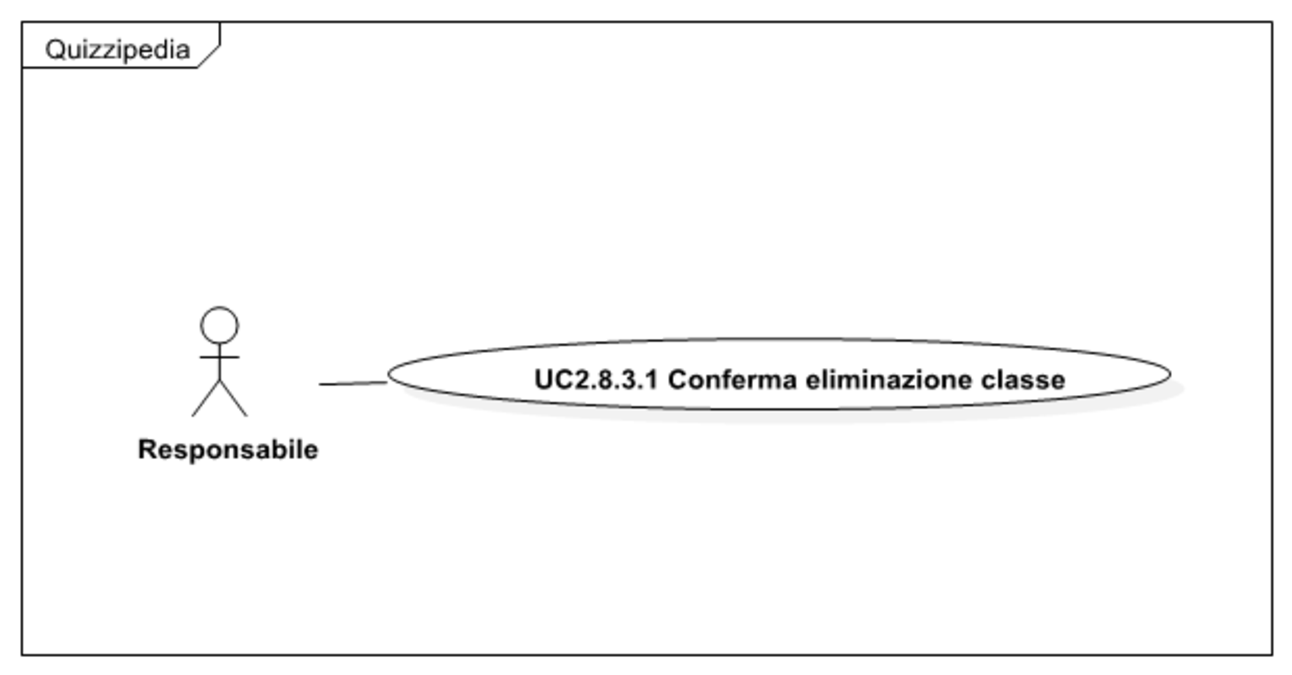
\includegraphics[width=\textwidth]{Img/UC Eliminazione classe.pdf}}
\caption{UC2.8.3 Eliminazione classe}
\end{figure}
\begin{itemize}
\item \textbf{Attori}: Responsabile.
\item \textbf{Scenario principale}:
\begin{enumerate}
\item Conferma eliminazione classe (UC2.8.3.1).
\end{enumerate}
\item \textbf{Descrizione}: il responsabile può eliminare una classe.
\item \textbf{Precondizione}: il responsabile ha i permessi per eliminare una classe.
\item \textbf{Postcondizione}: il responsabile ha eliminato la classe.
\end{itemize}
\subsubsection{UC2.8.3.1 Conferma eliminazione classe}
\begin{itemize}
\item \textbf{Attori}: Responsabile.
\item \textbf{Scenario principale}: il responsabile conferma l'eliminazione della classe.
\item \textbf{Descrizione}: il responsabile deve confermare l'eliminazione della classe.
\item \textbf{Precondizione}: il responsabile vuole eliminare una classe e deve ancora confermare.
\item \textbf{Postcondizione}: il responsabile ha confermato l'eliminazione della classe.
\end{itemize}
\subsubsection{UC2.8.4 Visualizza lista studenti della classe}
\begin{itemize}
\item \textbf{Attori}: Docente.
\item \textbf{Scenario principale}: il docente visualizza la lista degli studenti di una classe.
\item \textbf{Descrizione}: il docente seleziona il nome della classe e può visualizzare la lista di studenti associati a quella classe.
\item \textbf{Precondizione}: il responsabile e il docente hanno il permesso di consultare la lista degli studenti.
\item \textbf{Postcondizione}: vengono visualizzati gli studenti della classe selezionata.
\end{itemize}
\subsubsection{UC2.8.5 Visualizza lista docenti della classe}
\begin{itemize}
\item \textbf{Attori}: Responsabile.
\item \textbf{Scenario principale}: il responsabile visualizza la lista di docenti di una classe.
\item \textbf{Descrizione}: il responsabile seleziona il nome della classe e può visualizzare la lista di docenti associati a quella classe.
\item \textbf{Precondizione}: il responsabile ha il permesso di consultare la lista dei docenti.
\item \textbf{Postcondizione}: il responsabile visualizza i docenti della classe selezionata.
\end{itemize}
\subsubsection{UC2.8.6 Manutenzione classe}
\begin{figure}[H]
\centering
\noindent\makebox[\textwidth]{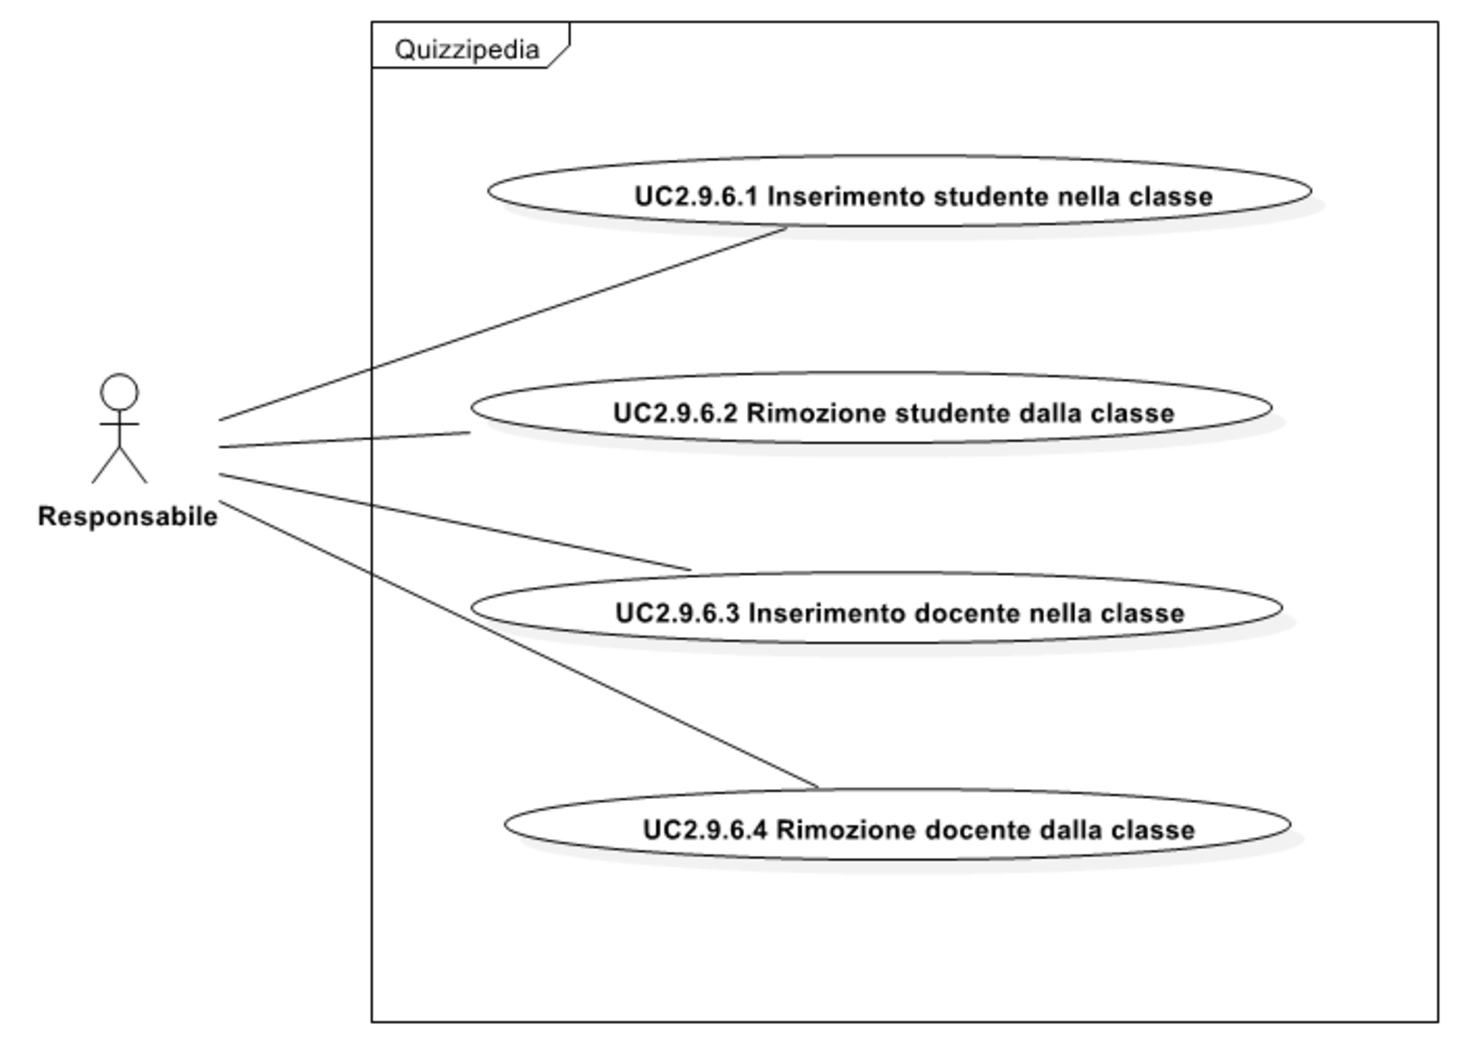
\includegraphics[width=\textwidth]{Img/UC Manutenzione classe.pdf}}
\caption{UC2.8.6 Manutenzione classe}
\end{figure}
\begin{itemize}
\item \textbf{Attori}: Responsabile.
\item \textbf{Scenario principale}:
\begin{enumerate}
\item Inserimento studente nella classe (UC2.8.6.1);
\item Rimozione studente dalla classe (UC2.8.6.2);
\item Inserimento docente nella classe (UC2.8.6.3);
\item Rimozione docente dalla classe (UC2.8.6.4).
\end{enumerate}
\item \textbf{Descrizione}: il responsabile può fare manutenzione su una classe nel caso in cui uno studente o un docente si sia inscritto in una classe sbagliata. Il responsabile procederà alla rimozione con successivo inserimento dello studente o del docente nella classe corretta.
\item \textbf{Precondizione}: il responsabile ha il permesso di fare manutenzione alla classe.
\item \textbf{Postcondizione}: il responsabile ha fatto alcune operazioni di manutenzione alla classe.
\end{itemize}
\subsubsection{UC2.8.6.1 Inserimento studente nella classe}
\begin{itemize}
\item \textbf{Attori}: Docente.
\item \textbf{Scenario principale}: il docente inserisce uno studente nella classe.
\item \textbf{Descrizione}: il docente può inserire uno studente nella classe.
\item \textbf{Precondizione}: il docente ha deciso di effettuare la manutenzione della classe.
\item \textbf{Postcondizione}: il docente ha inserito lo studente nella classe.
\end{itemize}
\subsubsection{UC2.8.6.2 Rimozione studente dalla classe}
\begin{itemize}
\item \textbf{Attori}: Docente.
\item \textbf{Scenario principale}: il docente rimuove uno studente dalla classe.
\item \textbf{Descrizione}: il docente può rimuovere uno studente dalla classe.
\item \textbf{Precondizione}: il docente ha deciso di effettuare la manutenzione della classe.
\item \textbf{Postcondizione}: il docente ha rimosso lo studente dalla classe.
\end{itemize}
\subsubsection{UC2.8.6.3 Inserimento docente nella classe}
\begin{itemize}
\item \textbf{Attori}: Responsabile.
\item \textbf{Scenario principale}: il responsabile inserisce un docente nella classe.
\item \textbf{Descrizione}: il responsabile può inserire un docente nella classe.
\item \textbf{Precondizione}: il responsabile ha deciso di effettuare la manutenzione della classe.
\item \textbf{Postcondizione}: il responsabile ha inserito il docente nella classe.
\end{itemize}
\subsubsection{UC2.8.6.4 Rimozione docente dalla classe}
\begin{itemize}
\item \textbf{Attori}: Responsabile.
\item \textbf{Scenario principale}: il responsabile rimuove un docente dalla classe.
\item \textbf{Descrizione}: il responsabile può rimuovere un docente dalla classe.
\item \textbf{Precondizione}: il responsabile ha deciso di effettuare la modifica della classe.
\item \textbf{Postcondizione}: il responsabile ha rimosso il docente dalla classe.
\end{itemize}
\subsubsection{UC2.9 Gestione richieste}
\begin{figure}[H]
\centering
\noindent\makebox[\textwidth]{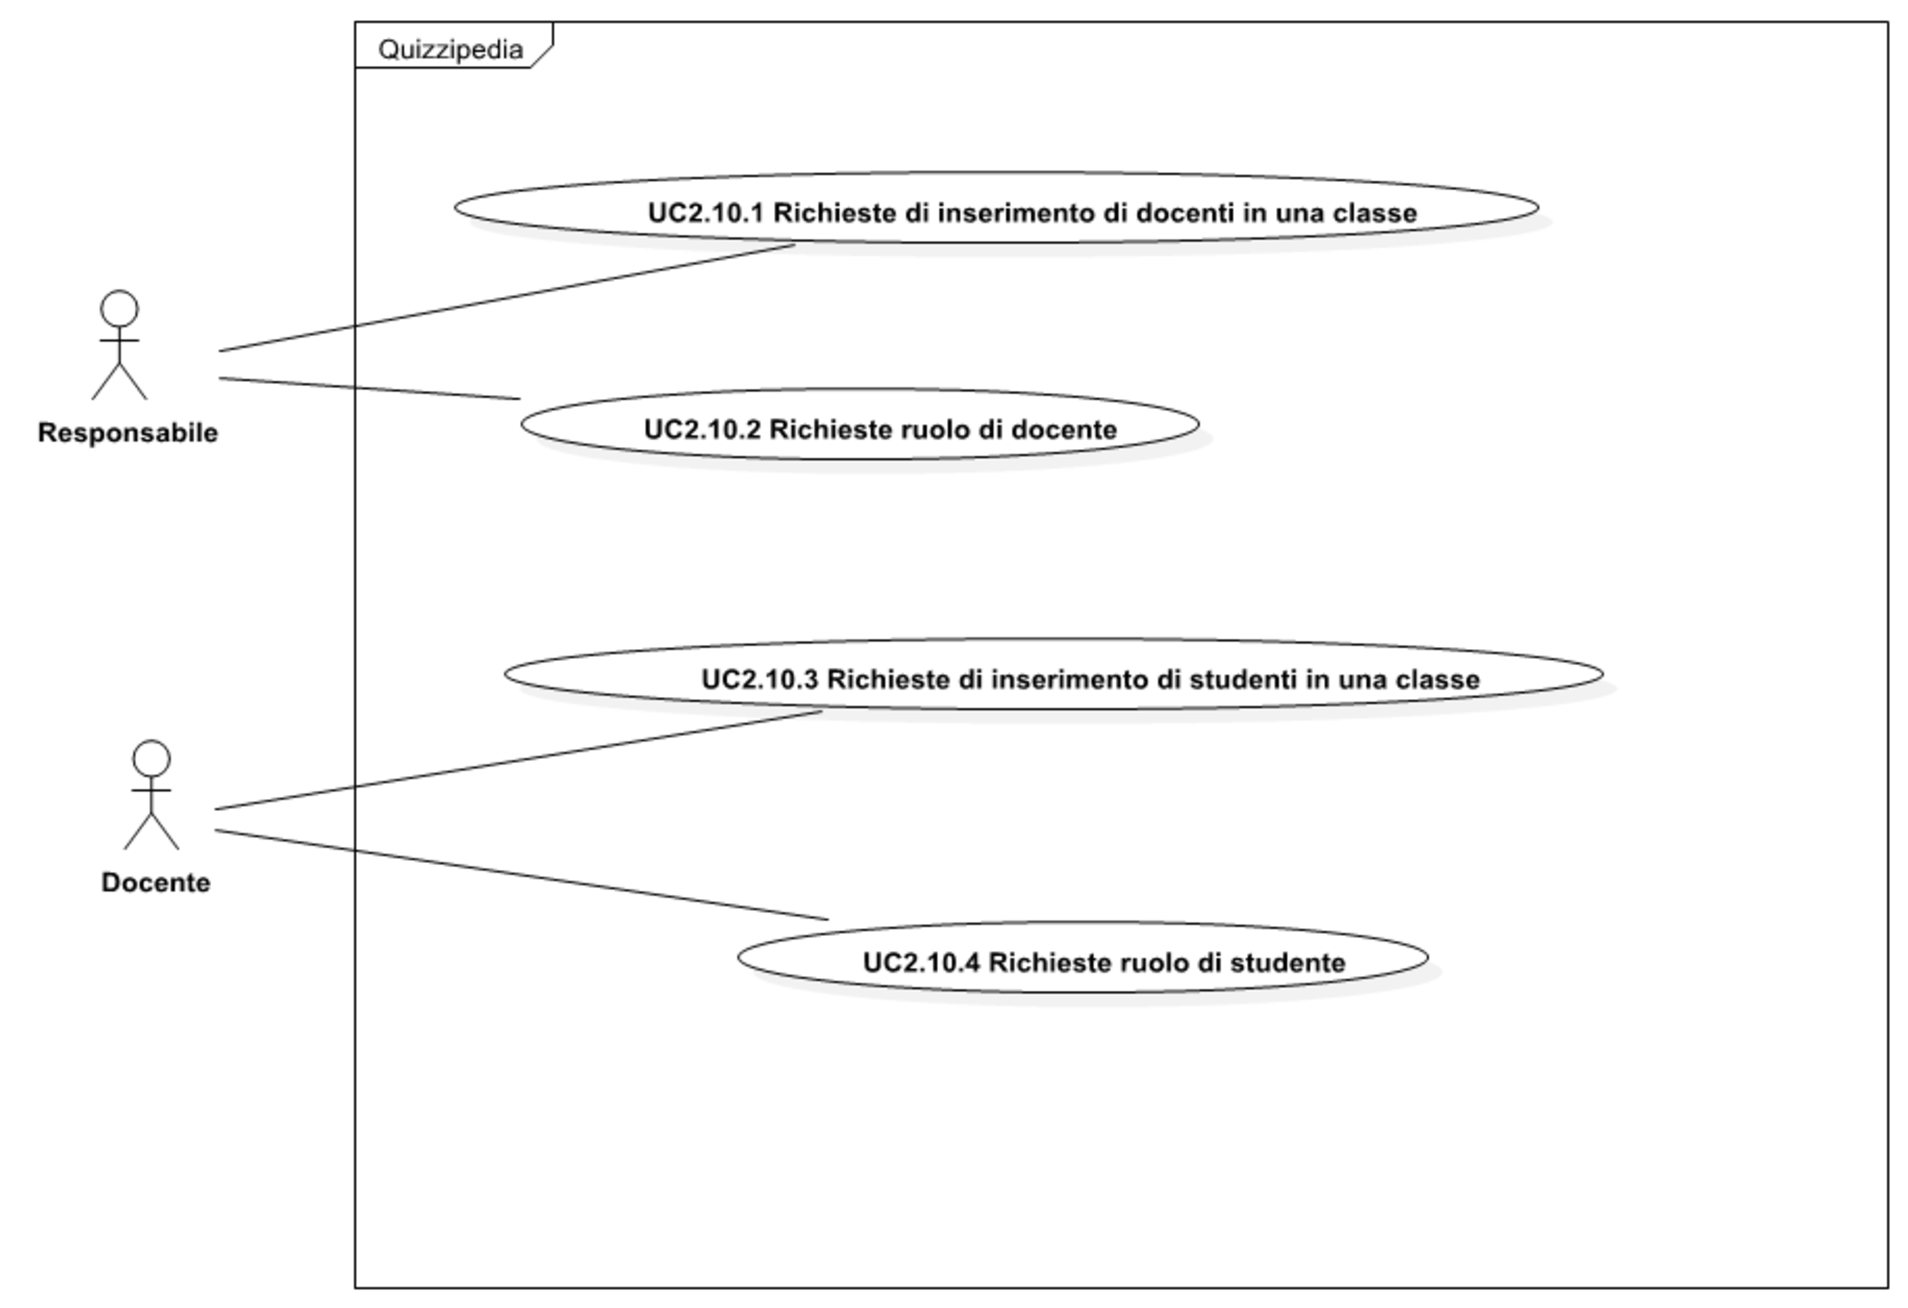
\includegraphics[width=\textwidth]{Img/UC Gestione richieste.pdf}}
\caption{UC2.9 Gestione richieste}
\end{figure}
\begin{itemize}
\item \textbf{Attori}: Docente, Responsabile.
\item \textbf{Scenario principale}:
\begin{enumerate}
\item Richieste di inserimento di docenti in una classe (UC2.9.1);
\item Richieste ruolo di docente (UC2.9.2);
\item Richieste di inserimento di studenti in una classe (UC2.9.3);
\item Richieste ruolo di studente (UC2.9.4).
\end{enumerate}
\item \textbf{Descrizione}: il responsabile gestisce le richieste inviate dai docenti, il docente gestisce le richieste inviate dagli studenti.
\item \textbf{Precondizione}: il responsabile e il docente sono autenticati.
\item \textbf{Postcondizione}: il responsabile e il docente hanno gestito le richieste presenti.
\end{itemize}
\subsubsection{UC2.9.1 Richieste di inserimento di docenti in una classe}
\begin{figure}[H]
\centering
\noindent\makebox[\textwidth]{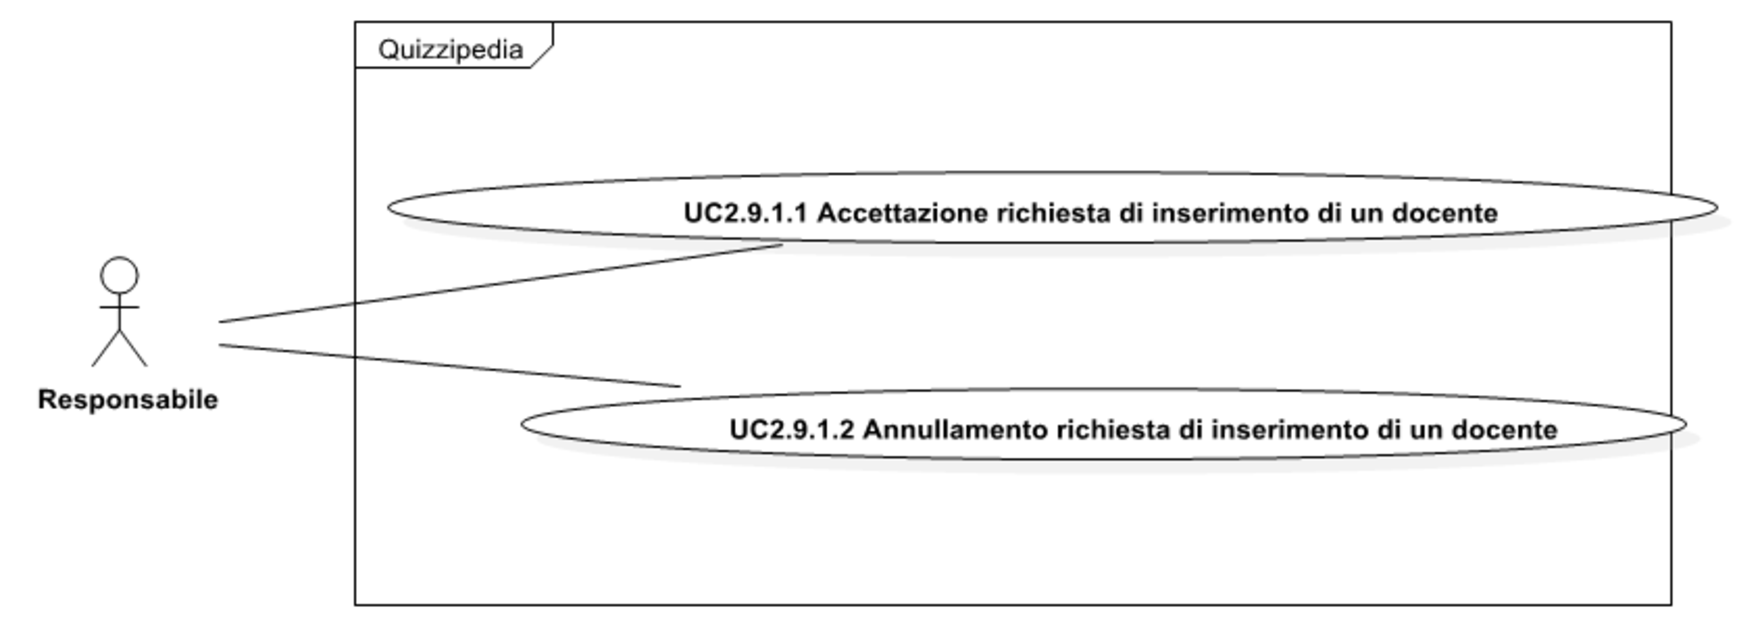
\includegraphics[width=\textwidth]{Img/UC Richieste di inserimento di docenti in una classe.pdf}}
\caption{UC2.9.1 Richieste di inserimento di docenti in una classe}
\end{figure}
\begin{itemize}
\item \textbf{Attori}: Responsabile.
\item \textbf{Scenario principale}:
\begin{enumerate}
\item Accettazione richiesta di inserimento di un docente (UC2.9.1.1);
\item Annullamento richiesta di inserimento di un docente (UC2.9.1.2).
\end{enumerate}
\item \textbf{Descrizione}: il responsabile accetta o rifiuta le richieste di inserimento in una classe appartenente al proprio ente ricevute dai docenti.
\item \textbf{Precondizione}: il responsabile visualizza la lista di richieste di inserimento nella classe da parte dei docenti.
\item \textbf{Postcondizione}: il responsabile ha accettato o rifiutato le richieste che ha ricevuto dai docenti.
\end{itemize}
\subsubsection{UC2.9.1.1 Accettazione richiesta di inserimento di un docente}
\begin{itemize}
\item \textbf{Attori}: Responsabile.
\item \textbf{Scenario principale}: il responsabile accetta la richiesta di inserimento nella classe da parte del docente.
\item \textbf{Descrizione}: il responsabile accetta la richiesta di inserimento nella classe ricevute da un docente.
\item \textbf{Precondizione}: il responsabile visualizza la lista delle richieste di inserimento nella classe da parte dei docenti.
\item \textbf{Postcondizione}: il responsabile ha accettato la richiesta di inserimento nella classe del docente.
\end{itemize}
\subsubsection{UC2.9.1.2 Annullamento richiesta di inserimento di un docente}
\begin{itemize}
\item \textbf{Attori}: Responsabile.
\item \textbf{Scenario principale}: il responsabile rifiuta le richieste di inserimento nella classe da parte dei docenti.
\item \textbf{Descrizione}: il responsabile rifiuta la richiesta di inserimento nella classe ricevuta da un docente.
\item \textbf{Precondizione}: il responsabile visualizza la lista delle richieste di inserimento nella classe da parte dei docenti.
\item \textbf{Postcondizione}: il responsabile ha rifiutato la richiesta di inserimento nella classe del docente.
\end{itemize}
\subsubsection{UC2.9.2 Richieste ruolo di docente}
\begin{figure}[H]
\centering
\noindent\makebox[\textwidth]{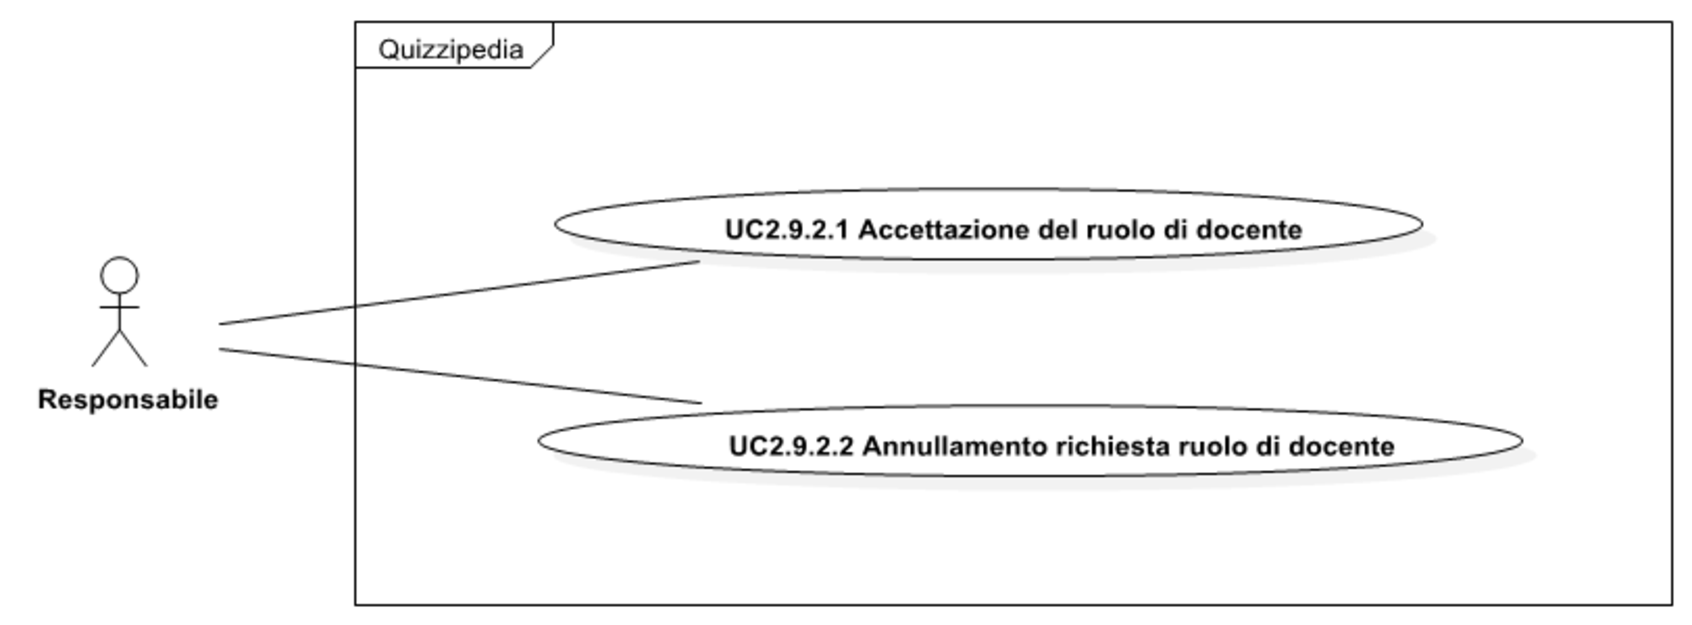
\includegraphics[width=\textwidth]{Img/UC Richieste ruolo di docente.pdf}}
\caption{UC2.9.2 Richieste ruolo di docente}
\end{figure}
\begin{itemize}
\item \textbf{Attori}: Responsabile.
\item \textbf{Scenario principale}:
\begin{enumerate}
\item Accettazione del ruolo di docente (UC2.9.2.1);
\item Annullamento richiesta ruolo di docente (UC2.9.2.2).
\end{enumerate}
\item \textbf{Descrizione}: il responsabile accetta o rifiuta le richieste del ruolo di docente che vogliono assumere gli utenti senza ruolo.
\item \textbf{Precondizione}: il responsabile ha i permessi per la gestione della lista richieste.
\item \textbf{Postcondizione}: il responsabile ha accettato o rifiutato le richieste del ruolo di docente che gli sono pervenute dagli utenti senza ruolo.
\end{itemize}
\subsubsection{UC2.9.2.1 Accettazione del ruolo di docente}
\begin{itemize}
\item \textbf{Attori}: Responsabile.
\item \textbf{Scenario principale}: il responsabile accetta le richieste di ruolo di docente.
\item \textbf{Descrizione}: il responsabile accetta  le richieste del ruolo di docente.
\item \textbf{Precondizione}: il responsabile visualizza la lista di richieste del ruolo di docente.
\item \textbf{Postcondizione}: il responsabile ha accettato le richieste del ruolo di docente.
\end{itemize}
\subsubsection{UC2.9.2.2 Annullamento richiesta ruolo di docente}
\begin{itemize}
\item \textbf{Attori}: Responsabile.
\item \textbf{Scenario principale}: il responsabile rifiuta le richieste di ruolo di docente.
\item \textbf{Descrizione}: il responsabile rifiuta le richieste del ruolo di docente.
\item \textbf{Precondizione}: il responsabile visualizza la lista di richieste del ruolo di docente.
\item \textbf{Postcondizione}: il responsabile ha rifiutato le richieste del ruolo di docente.
\end{itemize}
\subsubsection{UC2.9.3 Richieste di inserimento di studenti in una classe}
\begin{figure}[H]
\centering
\noindent\makebox[\textwidth]{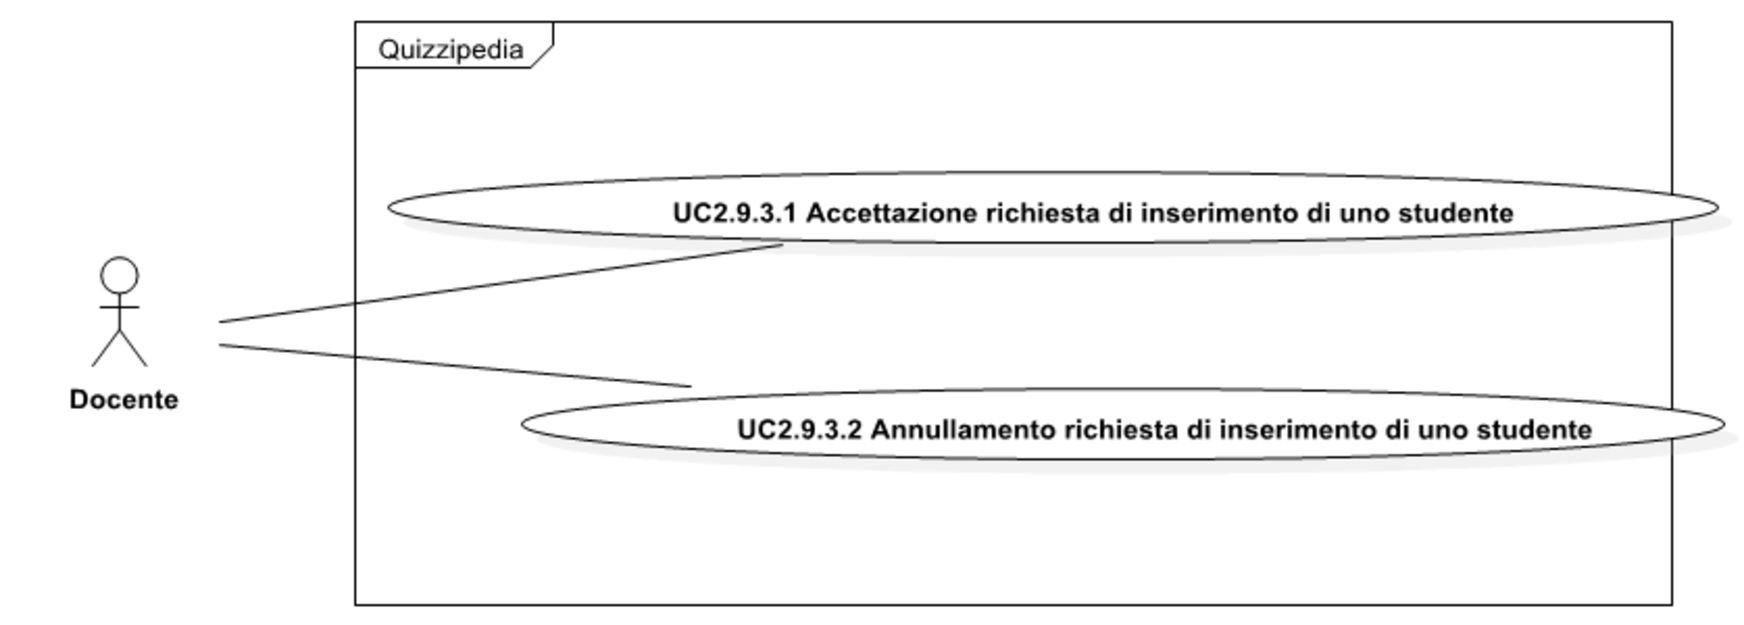
\includegraphics[width=\textwidth]{Img/UC Richieste di inserimento di studenti in una classe.pdf}}
\caption{UC2.9.3 Richieste di inserimento di studenti in una classe}
\end{figure}
\begin{itemize}
\item \textbf{Attori}: Docente.
\item \textbf{Scenario principale}:
\begin{enumerate}
\item Accettazione richiesta di inserimento di uno studente (UC2.9.3.1);
\item Annullamento richiesta di inserimento di uno studente (UC2.9.3.2).
\end{enumerate}
\item \textbf{Descrizione}: il docente può accettare o rifiutare le richieste di inserimento in una classe di cui è insegnante ricevute dagli studenti.
\item \textbf{Precondizione}: il docente visualizza la lista delle richieste di inserimento in una classe effettuate dagli studenti.
\item \textbf{Postcondizione}: il docente gestisce la richiesta di inserimento nella classe.
\end{itemize}
\subsubsection{UC2.9.3.1 Accettazione richiesta di inserimento di uno studente}
\begin{itemize}
\item \textbf{Attori}: Docente.
\item \textbf{Scenario principale}: il docente accetta la richieste di inserimento nella classe da parte dello studente.
\item \textbf{Descrizione}: il docente accetta la richiesta di inserimento nella classe ricevuta da uno studente.
\item \textbf{Precondizione}: il docente sta gestendo le richieste di inserimento nelle classi.
\item \textbf{Postcondizione}: il docente ha accettato la richiesta di inserimento nella classe dello studente.
\end{itemize}
\subsubsection{UC2.9.3.2 Annullamento richiesta di inserimento di uno studente}
\begin{itemize}
\item \textbf{Attori}: Docente.
\item \textbf{Scenario principale}: il docente rifiuta la richiesta di inserimento nella classe.
\item \textbf{Descrizione}: il docente rifiuta la richiesta di inserimento nella classe ricevute da uno studente.
\item \textbf{Precondizione}: il docente sta gestendo le richieste di inserimento nelle classi.
\item \textbf{Postcondizione}: il docente ha rifiutato la richiesta di inserimento nelle classi dello studente.
\end{itemize}
\subsubsection{UC2.9.4 Richieste ruolo di studente}
\begin{figure}[H]
\centering
\noindent\makebox[\textwidth]{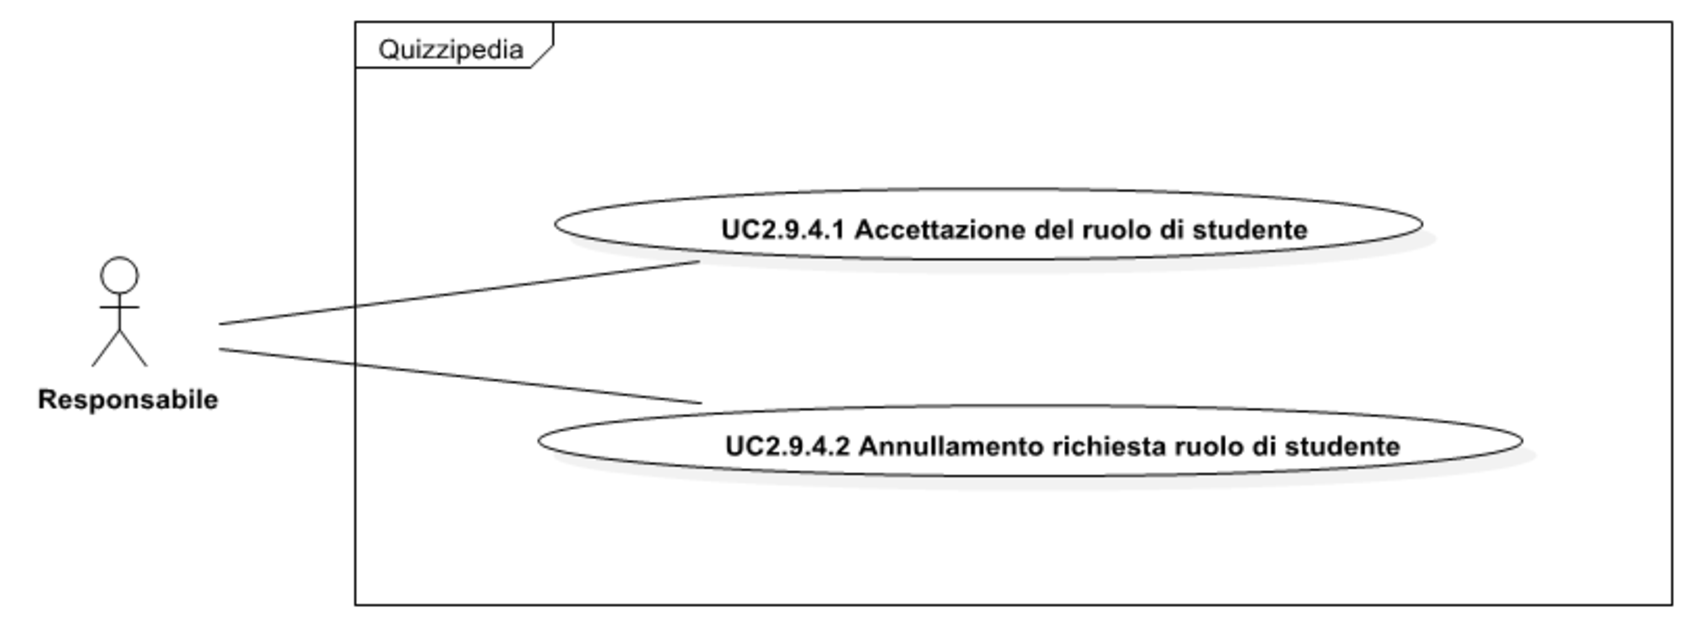
\includegraphics[width=\textwidth]{Img/UC Richieste ruolo di studente.pdf}}
\caption{UC2.9.4 Richieste ruolo di studente}
\end{figure}
\begin{itemize}
\item \textbf{Attori}: Responsabile.
\item \textbf{Scenario principale}:
\begin{enumerate}
\item Accettazione del ruolo di studente (UC2.9.4.1);
\item Annullamento richiesta ruolo di studente (UC2.9.4.2).
\end{enumerate}
\item \textbf{Descrizione}: il responsabile accetta o rifiuta le richieste del ruolo di studente pervenute dagli utenti senza ruolo.
\item \textbf{Precondizione}: il responsabile sta gestendo le richieste.
\item \textbf{Postcondizione}: il responsabile ha gestito le richieste di ruolo di studente che gli sono pervenute dagli utenti senza ruolo.
\end{itemize}
\subsubsection{UC2.9.4.1 Accettazione del ruolo di studente}
\begin{itemize}
\item \textbf{Attori}: Responsabile.
\item \textbf{Scenario principale}: il responsabile rifiuta le richieste di ruolo di studente.
\item \textbf{Descrizione}: il responsabile accetta le richieste del ruolo di studente.
\item \textbf{Precondizione}: il responsabile sta gestendo le richieste di ruolo di studente.
\item \textbf{Postcondizione}: il responsabile ha accettato le richieste di ruolo di studente.
\end{itemize}
\subsubsection{UC2.9.4.2 Annullamento richiesta ruolo di studente}
\begin{itemize}
\item \textbf{Attori}: Responsabile.
\item \textbf{Scenario principale}: il responsabile rifiuta le richieste di ruolo di studente.
\item \textbf{Descrizione}: il responsabile rifiuta le richieste di ruolo di studente.
\item \textbf{Precondizione}: il responsabile sta gestendo le richieste di ruolo di studente.
\item \textbf{Postcondizione}: il docente ha rifiutato le richieste di ruolo di studente.
\end{itemize}
\subsubsection{UC2.10 Gestione domande}
\begin{figure}[H]
\centering
\noindent\makebox[\textwidth]{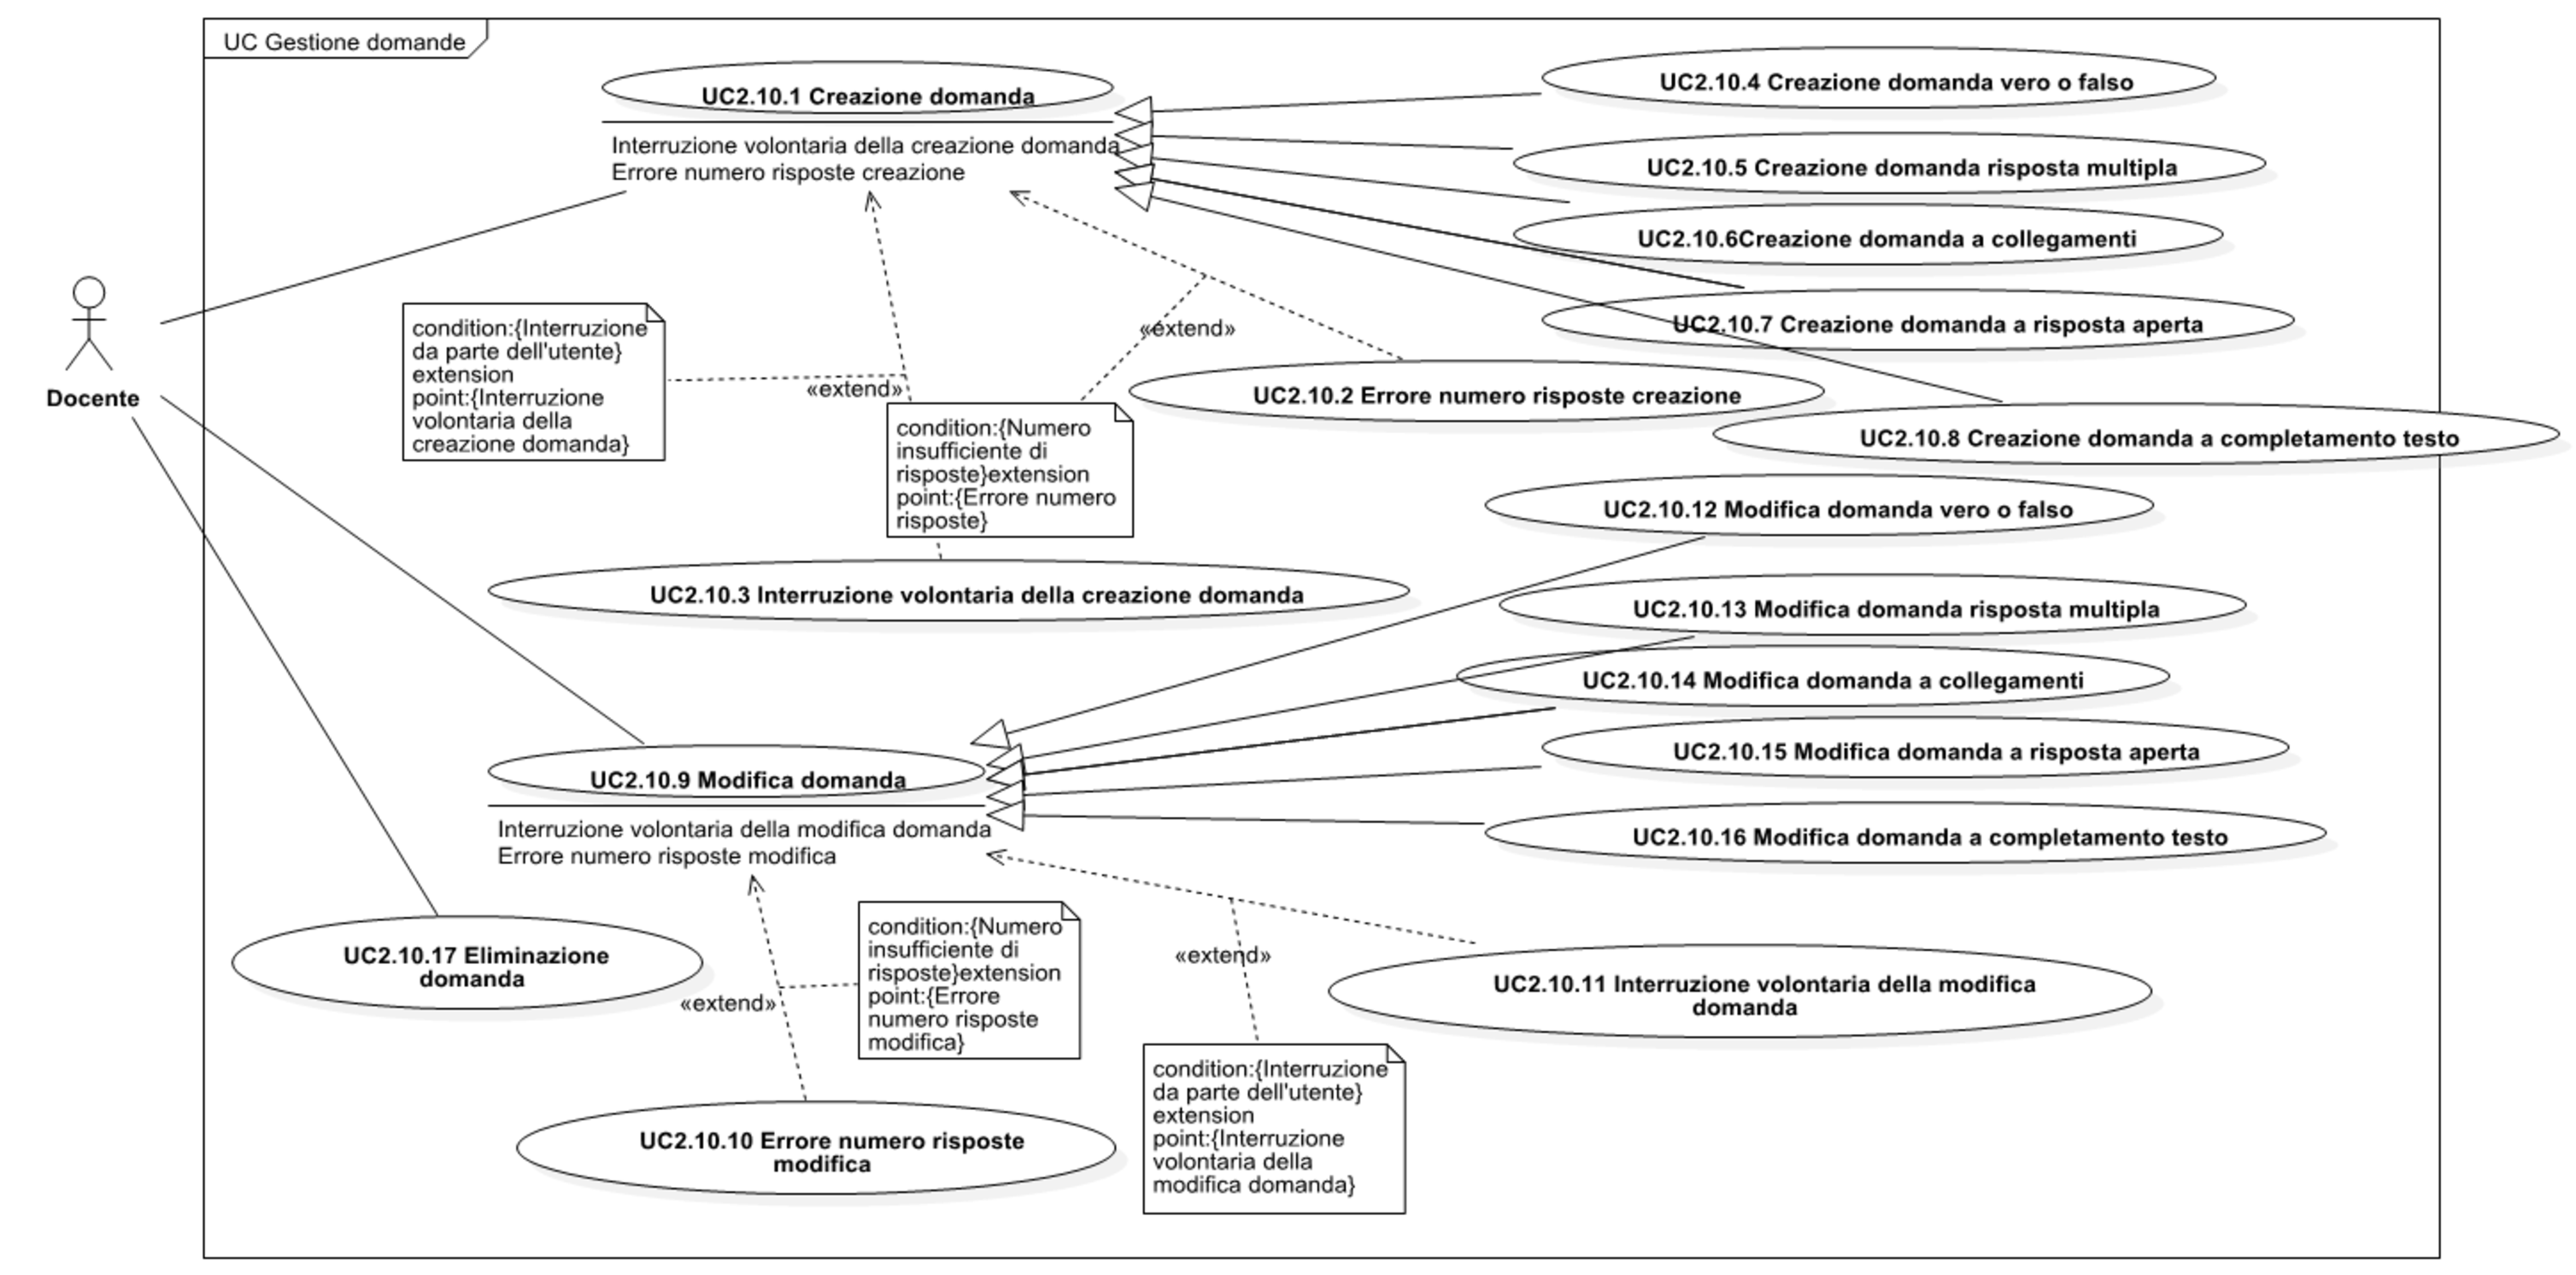
\includegraphics[width=\textwidth]{Img/UC Gestione domande.pdf}}
\caption{UC2.10 Gestione domande}
\end{figure}
\begin{itemize}
\item \textbf{Attori}: Docente.
\item \textbf{Scenario principale}:
\begin{enumerate}
\item Creazione domanda (UC2.10.1);
\item Errore numero risposte creazione (UC2.10.2);
\item Interruzione volontaria della creazione della domanda (UC2.10.3);
\item Creazione domanda vero o falso (UC2.10.4);
\item Creazione domanda risposta multipla (UC2.10.5);
\item Creazione domanda a collegamenti (UC2.10.6);
\item Creazione domanda a risposta aperta (UC2.10.7);
\item Creazione domanda a completamento testo (UC2.10.8);
\item Modifica domanda (UC2.10.9);
\item Errore numero risposte modifica (UC2.10.10);
\item Interruzione volontaria della modifica della domanda (UC2.10.11);
\item Modifica domanda vero o falso (UC2.10.12);
\item Modifica domanda risposta multipla (UC2.10.13);
\item Modifica domanda a risposta aperta (UC2.10.14);
\item Modifica domanda a completamento testo (UC2.10.15);
\item Modifica domanda a collegamenti (UC2.10.16);
\item Eliminazione domanda (UC2.10.17).
\end{enumerate}
\item \textbf{Descrizione}: il docente deve poter effettuare varie operazioni sulle domande, in particolare creare nuove domande di vario tipo e modificare o eliminare domande esistenti.
\item \textbf{Precondizione}: il sistema ha riconosciuto il docente e ora può gestire le domande.
\item \textbf{Postcondizione}: il docente ha completato le operazioni sulle domande con successo.
\end{itemize}
\subsubsection{UC2.10.1 Creazione domanda}
\begin{figure}[H]
\centering
\noindent\makebox[\textwidth]{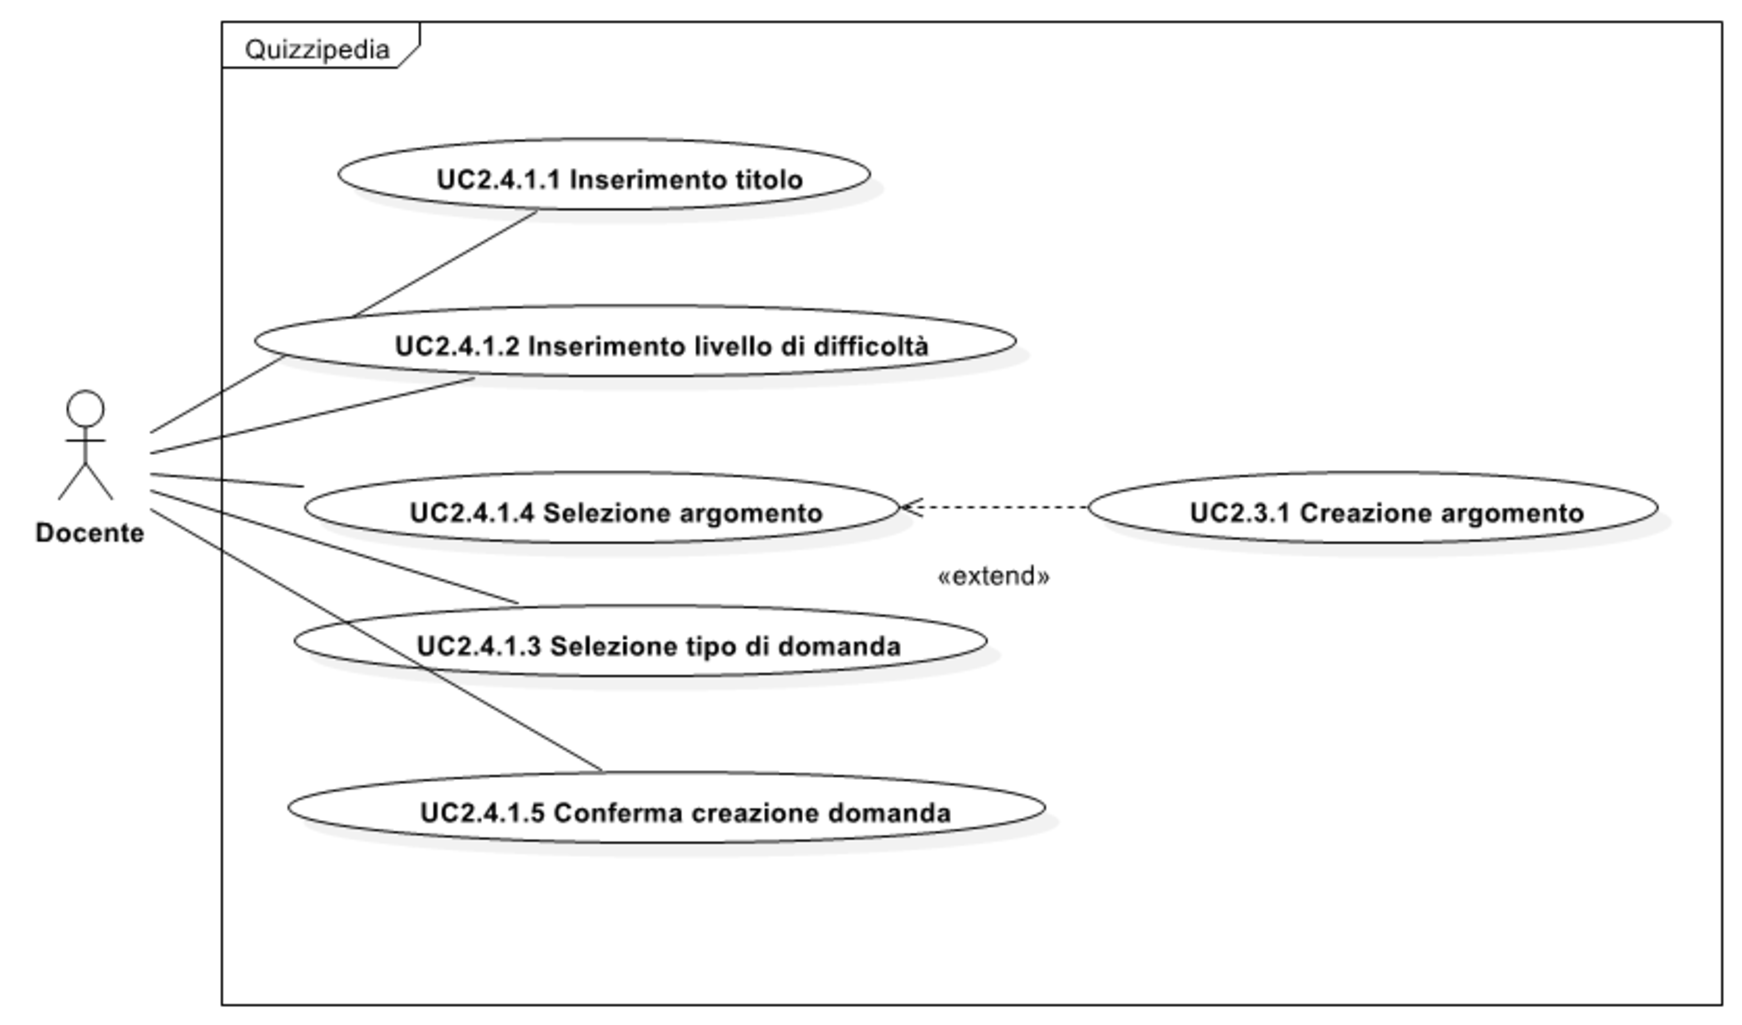
\includegraphics[width=\textwidth]{Img/UC Creazione domanda.pdf}}
\caption{UC2.10.1 Creazione domanda}
\end{figure}
\begin{itemize}
\item \textbf{Attori}: Docente.
\item \textbf{Scenario principale}:
\begin{enumerate}
\item Inserimento titolo domanda (UC2.10.1.1);
\item Descrizione aggiuntiva (UC2.10.1.2);
\item Selezione argomento della domanda (UC2.10.1.3);
\item Selezione livello di difficoltà (UC2.10.1.4);
\item Inserimento allegato (UC2.10.1.5);
\item Inserimento parole chiave (UC2.10.1.6).
\end{enumerate}
\item \textbf{Estensioni}:
\begin{itemize}
\item Errore numero risposte creazione (UC2.10.2);
\item Interruzione volontaria della creazione della domanda (UC2.10.3).
\end{itemize}
\item \textbf{Generalizzazioni}:
\begin{itemize}
\item Creazione domanda vero o falso (UC2.10.4);
\item Creazione domanda risposta multipla (UC2.10.5);
\item Creazione domanda a collegamenti (UC2.10.6);
\item Creazione domanda a risposta aperta (UC2.10.7);
\item Creazione domanda a completamento testo (UC2.10.8).
\end{itemize}
\item \textbf{Descrizione}: il docente deve poter creare una nuova domanda.
\item \textbf{Precondizione}: il docente è stato riconosciuto e vuole creare una nuova domanda.
\item \textbf{Postcondizione}: il docente ha creato una nuova domanda.
\end{itemize}
\subsubsection{UC2.10.1.1 Inserimento titolo domanda}
\begin{itemize}
\item \textbf{Attori}: Docente.
\item \textbf{Scenario principale}: il docente deve specificare il titolo della domanda.
\item \textbf{Descrizione}: il docente deve poter inserire il titolo della domanda.
\item \textbf{Precondizione}: il docente ha iniziato la creazione di una domanda e non ha ancora inserito il titolo.
\item \textbf{Postcondizione}: il docente ha inserito il titolo della domanda.
\end{itemize}
\subsubsection{UC2.10.1.2 Descrizione aggiuntiva}
\begin{itemize}
\item \textbf{Attori}: Docente.
\item \textbf{Scenario principale}: il docente inserisce una descrizione aggiuntiva.
\item \textbf{Descrizione}: il docente può inserire una descrizione aggiuntiva al titolo della domanda per renderla più comprensibile.
\item \textbf{Precondizione}: il docente ha iniziato la creazione di una domanda e non ha ancora inserito una descrizione aggiuntiva.
\item \textbf{Postcondizione}: il docente ha inserito una descrizione aggiuntiva.
\end{itemize}
\subsubsection{UC2.10.1.3 Selezione argomento della domanda}
\begin{itemize}
\item \textbf{Attori}: Docente.
\item \textbf{Scenario principale}: il docente seleziona l'argomento della domanda.
\item \textbf{Descrizione}: il docente deve selezionare l'argomento della domanda.
\item \textbf{Precondizione}: il docente ha iniziato la creazione di una domanda e non ha ancora selezionato l'argomento della domanda.
\item \textbf{Postcondizione}: il docente ha selezionato l'argomento della domanda.
\end{itemize}
\subsubsection{UC2.10.1.4 Selezione livello di difficoltà}
\begin{itemize}
\item \textbf{Attori}: Docente.
\item \textbf{Scenario principale}: il docente seleziona il livello di difficoltà della domanda.
\item \textbf{Descrizione}: il docente deve selezionare il livello di difficoltà della domanda.
\item \textbf{Precondizione}: il docente ha iniziato la creazione di una domanda e non ha ancora selezionato il livello di difficoltà della domanda.
\item \textbf{Postcondizione}: il docente ha selezionato il livello di difficoltà della domanda.
\end{itemize}
\subsubsection{UC2.10.1.5 Inserimento allegato}
\begin{figure}[H]
\centering
\noindent\makebox[\textwidth]{\includegraphics[width=\textwidth]{Img/UC Inserimento allegato.pdf}}
\caption{UC2.10.1.5 Inserimento allegato}
\end{figure}
\begin{itemize}
\item \textbf{Attori}: Docente.
\item \textbf{Scenario principale}:
\begin{enumerate}
\item Upload allegato (UC2.10.1.5.1).
\end{enumerate}
\item \textbf{Descrizione}: il docente può inserire un allegato che può essere una immagine o un video o un file audio.
\item \textbf{Precondizione}: il docente ha iniziato la creazione di una domanda e non ha ancora inserito l'allegato.
\item \textbf{Postcondizione}: il docente ha inserito l'allegato.
\end{itemize}
\subsubsection{UC2.10.1.5.1 Upload allegato}
\begin{itemize}
\item \textbf{Attori}: Docente.
\item \textbf{Scenario principale}: il docente esegue l'upload di una immagine o di un video o di un file audio.
\item \textbf{Descrizione}: il docente deve poter eseguire l'upload di una immagine o di un video o di un file audio.
\item \textbf{Precondizione}: il docente ha iniziato la creazione di una domanda e vuole inserire un allegato nella domanda ma non ha ancora fatto l'upload del file multimediale.
\item \textbf{Postcondizione}: il docente ha eseguito l'upload del file multimediale.
\end{itemize}
\subsubsection{UC2.10.1.6 Inserimento parole chiave}
\begin{itemize}
\item \textbf{Attori}: Docente.
\item \textbf{Scenario principale}: il docente specifica le parole chiave della domanda.
\item \textbf{Descrizione}: il docente deve poter inserire le parole chiave della domanda.
\item \textbf{Precondizione}: il docente ha iniziato la creazione di una domanda e non ha ancora inserito le parole chiave.
\item \textbf{Postcondizione}: il docente ha inserito le parole chiave.
\end{itemize}
\subsubsection{UC2.10.2 Errore numero risposte creazione}
\begin{itemize}
\item \textbf{Attori}: Docente.
\item \textbf{Scenario principale}: il docente non ha inserito il numero minimo di risposte nella domanda.
\item \textbf{Descrizione}: il docente non ha inserito il numero minimo di risposte nella domanda durante la creazione.
\item \textbf{Precondizione}: il docente ha creato una domanda con un numero di risposte minimo non valido.
\item \textbf{Postcondizione}: il docente visualizza il messaggio d'errore.
\end{itemize}
\subsubsection{UC2.10.3 Interruzione volontaria della creazione della domanda}
\begin{itemize}
\item \textbf{Attori}: Docente.
\item \textbf{Scenario principale}: il docente interrompe la creazione della domanda.
\item \textbf{Descrizione}: il docente sta creando una domanda, ma interrompe volontariamente la creazione.
\item \textbf{Precondizione}: il docente sta creando una domanda.
\item \textbf{Postcondizione}: la creazione della domanda è stata interrotta.
\end{itemize}
\subsubsection{UC2.10.4 Creazione domanda vero o falso}
\begin{figure}[H]
\centering
\noindent\makebox[\textwidth]{\includegraphics[width=\textwidth]{Img/UC Creazione domanda vero o falso.pdf}}
\caption{UC2.10.4 Creazione domanda vero o falso}
\end{figure}
\begin{itemize}
\item \textbf{Attori}: Docente.
\item \textbf{Scenario principale}:
\begin{enumerate}
\item Selezionare veridicità della domanda (UC2.10.4.1).
\end{enumerate}
\item \textbf{Descrizione}: il docente deve poter creare una nuova domanda del tipo vero o falso.
\item \textbf{Precondizione}: il docente è stato riconosciuto e vuole creare una nuova domanda del tipo vero o falso.
\item \textbf{Postcondizione}: il docente ha creato una nuova domanda del tipo vero o falso.
\item \textbf{Specializzazione di}:
\begin{enumerate}
\item Creazione domanda (UC2.10.1).
\end{enumerate}
\end{itemize}
\subsubsection{UC2.10.4.1 Selezionare veridicità della domanda}
\begin{itemize}
\item \textbf{Attori}: Docente.
\item \textbf{Scenario principale}: il docente seleziona la veridicità della domanda che sta creando.
\item \textbf{Descrizione}: il docente deve indicare la veridicità della domanda.
\item \textbf{Precondizione}: il docente ha iniziato la creazione di una domanda del tipo vero o falso e non ha ancora selezionato la veridicità della domanda.
\item \textbf{Postcondizione}: il docente ha indicato la veridicità della domanda.
\end{itemize}
\subsubsection{UC2.10.5 Creazione domanda risposta multipla}
\begin{figure}[H]
\centering
\noindent\makebox[\textwidth]{\includegraphics[width=\textwidth]{Img/UC Creazione domanda risposta multipla.pdf}}
\caption{UC2.10.5 Creazione domanda risposta multipla}
\end{figure}
\begin{itemize}
\item \textbf{Attori}: Docente.
\item \textbf{Scenario principale}:
\begin{enumerate}
\item Creazione risposta (UC2.10.5.1).
\end{enumerate}
\item \textbf{Descrizione}: il docente deve poter creare una nuova domanda a riposta multipla.
\item \textbf{Precondizione}: il docente è stato riconosciuto e vuole creare una nuova domanda a risposta multipla.
\item \textbf{Postcondizione}: il docente ha creato una nuova domanda a risposta multipla.
\item \textbf{Specializzazione di}:
\begin{enumerate}
\item Creazione domanda (UC2.10.1).
\end{enumerate}
\end{itemize}
\subsubsection{UC2.10.5.1 Creazione risposta}
\begin{figure}[H]
\centering
\noindent\makebox[\textwidth]{\includegraphics[width=\textwidth]{Img/UC Creazione risposta.pdf}}
\caption{UC2.10.5.1 Creazione risposta}
\end{figure}
\begin{itemize}
\item \textbf{Attori}: Docente.
\item \textbf{Scenario principale}:
\begin{enumerate}
\item Upload file multimediale (UC2.10.5.1.1);
\item Casella di testo (UC2.10.5.1.2);
\item Selezione veridicità della risposta (UC2.10.5.1.3).
\end{enumerate}
\item \textbf{Descrizione}: il docente deve poter creare risposte di vario tipo ad esempio: risposte testuali o con immagini o con video o con audio e successivamente indicare quali sono le risposte corrette.
\item \textbf{Precondizione}: il docente ha iniziato la creazione di una domanda a risposta multipla e non ha ancora creato le risposte alla domanda.
\item \textbf{Postcondizione}: il docente ha creato le risposte della domanda a risposta multipla.
\end{itemize}
\subsubsection{UC2.10.5.1.1 Upload file multimediale}
\begin{itemize}
\item \textbf{Attori}: Docente.
\item \textbf{Scenario principale}: il docente esegue l'upload di una immagine o di un video o di un file audio.
\item \textbf{Descrizione}: il docente deve poter eseguire l'upload di una immagine o di un video o di un file audio.
\item \textbf{Precondizione}: il docente ha iniziato a creare le risposte della domanda a risposta multipla ma non ha ancora eseguito l'upload del file multimediale.
\item \textbf{Postcondizione}: il docente ha eseguito l'upload del file multimediale.
\end{itemize}
\subsubsection{UC2.10.5.1.2 Casella di testo}
\begin{itemize}
\item \textbf{Attori}: Docente.
\item \textbf{Scenario principale}: il docente scrive la risposta testuale nella casella di testo.
\item \textbf{Inclusioni}:
\begin{itemize}
\item Selezione veridicità della risposta (UC2.10.5.1.3).
\end{itemize}
\item \textbf{Descrizione}: il docente deve poter inserire la risposta testuale nella casella di testo.
\item \textbf{Precondizione}: il docente ha iniziato a creare le risposte della domanda a risposta multipla ma non ha ancora inserito il testo della risposta.
\item \textbf{Postcondizione}: il docente ha inserito il testo della risposta.
\end{itemize}
\subsubsection{UC2.10.5.1.3 Selezione veridicità della risposta}
\begin{itemize}
\item \textbf{Attori}: Docente.
\item \textbf{Scenario principale}: il docente seleziona la veridicità della risposta che sta creando.
\item \textbf{Descrizione}: il docente deve selezionare la veridicità della risposta che sta creando.
\item \textbf{Precondizione}: il docente sta creando la risposta della domanda a risposta multipla ma non ha ancora selezionato la veridicità della risposta.
\item \textbf{Postcondizione}: il docente ha indicato la veridicità della risposta.
\end{itemize}
\subsubsection{UC2.10.6 Creazione domanda a collegamenti}
\begin{figure}[H]
\centering
\noindent\makebox[\textwidth]{\includegraphics[width=\textwidth]{Img/UC Creazione domanda a collegamenti.pdf}}
\caption{UC2.10.6 Creazione domanda a collegamenti}
\end{figure}
\begin{itemize}
\item \textbf{Attori}: Docente.
\item \textbf{Scenario principale}:
\begin{enumerate}
\item Creazione ennupla (UC2.10.6.1).
\end{enumerate}
\item \textbf{Descrizione}: il docente deve poter creare una nuova domanda a collegamenti.
\item \textbf{Precondizione}: il docente è stato riconosciuto e vuole creare una nuova domanda a collegamenti.
\item \textbf{Postcondizione}: il docente ha creato una nuova domanda a collegamenti.
\item \textbf{Specializzazione di}:
\begin{enumerate}
\item Creazione domanda (UC2.10.1).
\end{enumerate}
\end{itemize}
\subsubsection{UC2.10.6.1 Creazione ennupla}
\begin{figure}[H]
\centering
\noindent\makebox[\textwidth]{\includegraphics[width=\textwidth]{Img/UC Creazione ennupla.pdf}}
\caption{UC2.10.6.1 Creazione ennupla}
\end{figure}
\begin{itemize}
\item \textbf{Attori}: Docente.
\item \textbf{Scenario principale}:
\begin{enumerate}
\item Inserire parte iniziale (UC2.10.6.1.1);
\item Inserire parte finale (UC2.10.6.1.2).
\end{enumerate}
\item \textbf{Descrizione}: il docente può inserire la parte iniziale e finale della risposta oppure può solo inserire la parta finale, lasciando vuota quella iniziale, che corrisponderà a una risposta sbagliata.
\item \textbf{Precondizione}: il docente ha iniziato la creazione della domanda a collegamenti ma non ha ancora creato l'ennupla della risposta.
\item \textbf{Postcondizione}: il docente ha inserito l'ennupla della risposta.
\end{itemize}
\subsubsection{UC2.10.6.1.1 Inserire parte iniziale}
\begin{figure}[H]
\centering
\noindent\makebox[\textwidth]{\includegraphics[width=\textwidth]{Img/UC Inserire parte iniziale.pdf}}
\caption{UC2.10.6.1.1 Inserire parte iniziale}
\end{figure}
\begin{itemize}
\item \textbf{Attori}: Docente.
\item \textbf{Scenario principale}:
\begin{enumerate}
\item Upload file della parte iniziale della risposta (UC2.10.6.1.1.1);
\item Inserire testo della parte iniziale della risposta (UC2.10.6.1.1.2).
\end{enumerate}
\item \textbf{Descrizione}: il docente può inserire come parte iniziale della risposta un file multimediale (immagine, video, audio), oppure inserire una risposta testuale.
\item \textbf{Precondizione}: il docente ha iniziato la creazione della risposta ma non ha ancora inserito la parte iniziale della risposta.
\item \textbf{Postcondizione}: il docente ha inserito la parte iniziale della risposta.
\end{itemize}
\subsubsection{UC2.10.6.1.1.1 Upload file della parte iniziale della risposta}
\begin{itemize}
\item \textbf{Attori}: Docente.
\item \textbf{Scenario principale}: il docente può inserire il file multimediale della parte iniziale della risposta, facendo l'upload del file.
\item \textbf{Descrizione}: il docente deve poter inserire il file multimediale della parte iniziale della risposta, eseguendo l'upload del file.
\item \textbf{Precondizione}: il docente ha iniziato a creare la parte iniziale della risposta ma non ha ancora fatto l'upload del file multimediale.
\item \textbf{Postcondizione}: il docente ha eseguito l'upload del file multimediale.
\end{itemize}
\subsubsection{UC2.10.6.1.1.2 Inserire testo della parte iniziale della risposta}
\begin{itemize}
\item \textbf{Attori}: Docente.
\item \textbf{Scenario principale}: il docente può inserisce il testo della parte iniziale della risposta.
\item \textbf{Descrizione}: il docente deve poter inserire il testo della parte iniziale della risposta.
\item \textbf{Precondizione}: il docente ha iniziato la creazione della parte iniziale della risposta ma non ha ancora inserito il testo della risposta.
\item \textbf{Postcondizione}: il docente ha inserito il testo della parte iniziale della risposta.
\end{itemize}
\subsubsection{UC2.10.6.1.2 Inserire parte finale}
\begin{figure}[H]
\centering
\noindent\makebox[\textwidth]{\includegraphics[width=\textwidth]{Img/UC Inserire parte finale.pdf}}
\caption{UC2.10.6.1.2 Inserire parte finale}
\end{figure}
\begin{itemize}
\item \textbf{Attori}: Docente.
\item \textbf{Scenario principale}:
\begin{enumerate}
\item Upload file della parte finale della risposta (UC2.10.6.1.2.1);
\item Inserire testo della parte finale della risposta (UC2.10.6.1.2.2).
\end{enumerate}
\item \textbf{Descrizione}: il docente può inserire come parte finale della risposta un file multimediale (immagine, video, audio), oppure inserire una risposta testuale.
\item \textbf{Precondizione}: il docente ha iniziato la creazione della risposta ma non ha ancora inserito la parte finale della risposta.
\item \textbf{Postcondizione}: il docente ha inserito la parte finale della risposta.
\end{itemize}
\subsubsection{UC2.10.6.1.2.1 Upload file della parte finale della risposta}
\begin{itemize}
\item \textbf{Attori}: Docente.
\item \textbf{Scenario principale}: il docente può inserire il file multimediale della parte finale della risposta, facendo l'upload del file.
\item \textbf{Descrizione}: il docente deve poter inserire il file multimediale della parte finale della risposta, eseguendo l'upload del file.
\item \textbf{Precondizione}: il docente ha iniziato la creazione della parte finale della risposta ma non ha ancora fatto l'upload del file multimediale.
\item \textbf{Postcondizione}: il docente ha eseguito l'upload del file multimediale.
\end{itemize}
\subsubsection{UC2.10.6.1.2.2 Inserire testo della parte finale della risposta}
\begin{itemize}
\item \textbf{Attori}: Docente.
\item \textbf{Scenario principale}: il docente può inserisce il testo della parte finale della risposta.
\item \textbf{Descrizione}: il docente deve poter inserire il testo della parte finale della risposta.
\item \textbf{Precondizione}: il docente ha iniziato la creazione della parte finale della risposta ma non ha ancora inserito il testo della risposta.
\item \textbf{Postcondizione}: il docente ha inserito il testo della parte finale della risposta.
\end{itemize}
\subsubsection{UC2.10.7 Creazione domanda a risposta aperta}
\begin{figure}[H]
\centering
\noindent\makebox[\textwidth]{\includegraphics[width=\textwidth]{Img/UC Creazione domanda a risposta aperta.pdf}}
\caption{UC2.10.7 Creazione domanda a risposta aperta}
\end{figure}
\begin{itemize}
\item \textbf{Attori}: Docente.
\item \textbf{Scenario principale}:
\begin{enumerate}
\item Inserire la risposta corretta (UC2.10.7.1).
\end{enumerate}
\item \textbf{Descrizione}: il docente deve poter creare una nuova domanda a risposta aperta.
\item \textbf{Precondizione}: il docente è stato riconosciuto e vuole creare una nuova domanda a risposta aperta.
\item \textbf{Postcondizione}: il docente ha creato una nuova domanda a risposta aperta.
\item \textbf{Specializzazione di}:
\begin{enumerate}
\item Creazione domanda (UC2.10.1).
\end{enumerate}
\end{itemize}
\subsubsection{UC2.10.7.1 Inserire la risposta corretta}
\begin{itemize}
\item \textbf{Attori}: Docente.
\item \textbf{Scenario principale}: il docente specifica la risposta corretta alla domanda.
\item \textbf{Descrizione}: il docente inserisce la risposta corretta alla domanda.
\item \textbf{Precondizione}: il docente ha iniziato la creazione di una domanda a risposta aperta ma non ha ancora specificato la risposta corretta.
\item \textbf{Postcondizione}: il docente ha inserito la risposta corretta alla domanda.
\end{itemize}
\subsubsection{UC2.10.8 Creazione domanda a completamento testo}
\begin{figure}[H]
\centering
\noindent\makebox[\textwidth]{\includegraphics[width=\textwidth]{Img/UC Creazione domanda a completamento testo.pdf}}
\caption{UC2.10.8 Creazione domanda a completamento testo}
\end{figure}
\begin{itemize}
\item \textbf{Attori}: Docente.
\item \textbf{Scenario principale}:
\begin{enumerate}
\item Inserire testo incompleto (UC2.10.8.1);
\item Inserire insieme di parole (UC2.10.8.2).
\end{enumerate}
\item \textbf{Descrizione}: il docente deve poter creare una nuova domanda a completamento testo.
\item \textbf{Precondizione}: il docente è stato riconosciuto e vuole creare una nuova domanda a completamento testo.
\item \textbf{Postcondizione}: il docente ha creato una nuova domanda a completamento testo.
\item \textbf{Specializzazione di}:
\begin{enumerate}
\item Creazione domanda (UC2.10.1).
\end{enumerate}
\end{itemize}
\subsubsection{UC2.10.8.1 Inserire testo incompleto}
\begin{itemize}
\item \textbf{Attori}: Docente.
\item \textbf{Scenario principale}: il docente inserisce il testo incompleto della domanda, specificando gli spazi vuoti nel testo.
\item \textbf{Descrizione}: il docente deve poter inserire il testo incompleto della domanda, specificando gli spazi vuoti.
\item \textbf{Precondizione}: il docente ha iniziato la creazione di una domanda a completamento testo ma non ha ancora inserito il testo incompleto della domanda.
\item \textbf{Postcondizione}: il docente ha inserito il testo incompleto della domanda.
\end{itemize}
\subsubsection{UC2.10.8.2 Inserire insieme di parole}
\begin{itemize}
\item \textbf{Attori}: Docente.
\item \textbf{Scenario principale}: il docente inserisce un insieme di parole che sono corrette e sbagliate.
\item \textbf{Descrizione}: il docente deve specificare un insieme di parole che sono corrette e sbagliate.
\item \textbf{Precondizione}:  il docente ha iniziato la creazione di una domanda a completamento testo ma non ha ancora inserito l'insieme di parole corrette e sbagliate.
\item \textbf{Postcondizione}: il docente ha inserito l'insieme di parole corrette e sbagliate.
\end{itemize}
\subsubsection{UC2.10.9 Modifica domanda}
\begin{figure}[H]
\centering
\noindent\makebox[\textwidth]{\includegraphics[width=\textwidth]{Img/UC Modifica domanda.pdf}}
\caption{UC2.10.9 Modifica domanda}
\end{figure}
\begin{itemize}
\item \textbf{Attori}: Docente.
\item \textbf{Scenario principale}:
\begin{enumerate}
\item Modifica titolo domanda
 (UC2.10.9.1);
\item Modifica descrizione aggiuntiva (UC2.10.9.2);
\item Modifica argomento della domanda (UC2.10.9.3);
\item Modifica livello difficoltà (UC2.10.9.4);
\item Modifica allegato (UC2.10.9.5);
\item Modifica parole chiave (UC2.10.9.6).
\end{enumerate}
\item \textbf{Estensioni}:
\begin{itemize}
\item Errore numero risposte modifica (UC2.10.10);
\item Interruzione volontaria della modifica della domanda (UC2.10.11).
\end{itemize}
\item \textbf{Generalizzazioni}:
\begin{itemize}
\item Modifica domanda vero o falso (UC2.10.12);
\item Modifica domanda risposta multipla (UC2.10.13);
\item Modifica domanda a risposta aperta (UC2.10.14);
\item Modifica domanda a completamento testo (UC2.10.15);
\item Modifica domanda a collegamenti (UC2.10.16).
\end{itemize}
\item \textbf{Descrizione}: il docente deve poter modificare una domanda da lui creata.
\item \textbf{Precondizione}: il docente è stato riconosciuto e vuole modificare una domanda da lui creata
.
\item \textbf{Postcondizione}: il docente ha modificato una domanda esistente da lui creata.
\end{itemize}
\subsubsection{UC2.10.9.1 Modifica titolo domanda
}
\begin{itemize}
\item \textbf{Attori}: Docente.
\item \textbf{Scenario principale}: il docente può modificare il titolo della domanda che ha selezionato.
\item \textbf{Descrizione}: il docente deve poter modificare il titolo della domanda che ha selezionato.
\item \textbf{Precondizione}: il docente ha iniziato la modifica di una domanda ma non ha ancora modificato il titolo
.
\item \textbf{Postcondizione}: il docente ha modificato il titolo della domanda.
\end{itemize}
\subsubsection{UC2.10.9.2 Modifica descrizione aggiuntiva}
\begin{itemize}
\item \textbf{Attori}: Docente.
\item \textbf{Scenario principale}: il docente può modificare la descrizione aggiuntiva della domanda selezionata.
\item \textbf{Descrizione}: il docente deve poter modificare la descrizione aggiuntiva della domanda selezionata.
\item \textbf{Precondizione}: il docente ha iniziato la modifica di una domanda ma non ha ancora modificato la descrizione aggiuntiva.
\item \textbf{Postcondizione}: il docente ha modificato la descrizione aggiuntiva.
\end{itemize}
\subsubsection{UC2.10.9.3 Modifica argomento della domanda}
\begin{itemize}
\item \textbf{Attori}: Docente.
\item \textbf{Scenario principale}: il docente può modificare l'argomento della domanda selezionata semplicemente selezionando un argomento tra quelli disponibili.
\item \textbf{Descrizione}: il docente deve poter modificare l'argomento della domanda selezionata semplicemente selezionando un argomento tra quelli disponibili.
\item \textbf{Precondizione}: il docente ha iniziato la modifica di una domanda ma non ha ancora modificato l'argomento della domanda.
\item \textbf{Postcondizione}: il docente ha modificato l'argomento della domanda selezionata.
\end{itemize}
\subsubsection{UC2.10.9.4 Modifica livello difficoltà}
\begin{itemize}
\item \textbf{Attori}: Docente.
\item \textbf{Scenario principale}: il docente può modificare il livello di difficoltà della domanda selezionata.
\item \textbf{Descrizione}: il docente deve poter modificare il livello di difficoltà della domanda selezionata.
\item \textbf{Precondizione}: il docente ha iniziato la modifica di una domanda ma non ha ancora modificato il livello di difficoltà.
\item \textbf{Postcondizione}: il docente ha modificato il livello di difficoltà della domanda selezionata.
\end{itemize}
\subsubsection{UC2.10.9.5 Modifica allegato}
\begin{itemize}
\item \textbf{Attori}: Docente.
\item \textbf{Scenario principale}: il docente può modificare l'allegato della domanda eseguendo l'upload di un file multimediale (immagine, audio, video).
\item \textbf{Descrizione}: il docente ha la possibilità di modificare l'allegato della domanda eseguendo l'upload di un file multimediale.
\item \textbf{Precondizione}: il docente ha iniziato la modifica di una domanda ma non ha ancora modificato l'allegato della domanda.
\item \textbf{Postcondizione}: il docente ha modificato l'allegato della domanda.
\end{itemize}
\subsubsection{UC2.10.9.6 Modifica parole chiave}
\begin{itemize}
\item \textbf{Attori}: Docente.
\item \textbf{Scenario principale}: il docente modifica le parole chiave della domanda.
\item \textbf{Descrizione}: il docente deve poter modificare le parole chiave della domanda che sta modificando.
\item \textbf{Precondizione}: il docente ha iniziato la modifica di una domanda ma non ha ancora modificato le parole chiave.
\item \textbf{Postcondizione}: il docente ha modificato le parole chiave.
\end{itemize}
\subsubsection{UC2.10.10 Errore numero risposte modifica}
\begin{itemize}
\item \textbf{Attori}: Docente.
\item \textbf{Scenario principale}: il docente durante la modifica di una domanda non ha lasciato un numero minimo di risposte valide.
\item \textbf{Descrizione}: il docente durante la modifica di una domanda non ha lasciato un numero minimo di risposte valide
.
\item \textbf{Precondizione}: il docente ha modificato una domanda ed ha un numero di risposte non valido.
\item \textbf{Postcondizione}: il docente visualizza il messaggio d'errore.
\end{itemize}
\subsubsection{UC2.10.11 Interruzione volontaria della modifica della domanda}
\begin{itemize}
\item \textbf{Attori}: Docente.
\item \textbf{Scenario principale}: il docente interrompe la modifica della domanda.
\item \textbf{Descrizione}: il docente sta modificando una domanda, ma interrompe volontariamente la modifica.
\item \textbf{Precondizione}: il docente sta modificando una domanda.
\item \textbf{Postcondizione}: la modifica della domanda è stata interrotta.
\end{itemize}
\subsubsection{UC2.10.12 Modifica domanda vero o falso}
\begin{figure}[H]
\centering
\noindent\makebox[\textwidth]{\includegraphics[width=\textwidth]{Img/UC Modifica domanda vero o falso.pdf}}
\caption{UC2.10.12 Modifica domanda vero o falso}
\end{figure}
\begin{itemize}
\item \textbf{Attori}: Docente.
\item \textbf{Scenario principale}:
\begin{enumerate}
\item Modifica veridicità della domanda (UC2.10.12.1).
\end{enumerate}
\item \textbf{Descrizione}: il docente deve poter modificare una domanda del tipo vero o falso da lui creata.
\item \textbf{Precondizione}: il docente è stato riconosciuto e vuole modificare una domanda vero o falso da lui creata.
\item \textbf{Postcondizione}: il docente ha modificato una domanda del tipo vero o falso esistente da lui creata.
\item \textbf{Specializzazione di}:
\begin{enumerate}
\item Modifica domanda (UC2.10.9).
\end{enumerate}
\end{itemize}
\subsubsection{UC2.10.12.1 Modifica veridicità della domanda}
\begin{itemize}
\item \textbf{Attori}: Docente.
\item \textbf{Scenario principale}: il docente deve poter modificare la veridicità della domanda che sta modificando.
\item \textbf{Descrizione}: il docente può modificare la veridicità della domanda che sta modificando.
\item \textbf{Precondizione}: il docente ha iniziato la modifica di una domanda del tipo vero o falso ma non ha ancora modificato la veridicità della domanda.
\item \textbf{Postcondizione}: il docente ha modificato la veridicità della domanda.
\end{itemize}
\subsubsection{UC2.10.13 Modifica domanda risposta multipla}
\begin{figure}[H]
\centering
\noindent\makebox[\textwidth]{\includegraphics[width=\textwidth]{Img/UC Modifica domanda risposta multipla.pdf}}
\caption{UC2.10.13 Modifica domanda risposta multipla}
\end{figure}
\begin{itemize}
\item \textbf{Attori}: Docente.
\item \textbf{Scenario principale}:
\begin{enumerate}
\item Aggiungere una risposta (UC2.10.13.1);
\item Modificare una risposta (UC2.10.13.2);
\item Eliminare una risposta (UC2.10.13.3).
\end{enumerate}
\item \textbf{Descrizione}: il docente deve poter modificare una domanda a risposta multipla da lui creata.
\item \textbf{Precondizione}: il docente è stato riconosciuto e vuole modificare una domanda a risposta multipla da lui creata.
\item \textbf{Postcondizione}: il docente ha modificato una domanda a risposta multipla.
\item \textbf{Specializzazione di}:
\begin{enumerate}
\item Modifica domanda (UC2.10.9).
\end{enumerate}
\end{itemize}
\subsubsection{UC2.10.13.1 Aggiungere una risposta}
\begin{figure}[H]
\centering
\noindent\makebox[\textwidth]{\includegraphics[width=\textwidth]{Img/UC Aggiungere una risposta.pdf}}
\caption{UC2.10.13.1 Aggiungere una risposta}
\end{figure}
\begin{itemize}
\item \textbf{Attori}: Docente.
\item \textbf{Scenario principale}:
\begin{enumerate}
\item Upload file multimediale della risposta (UC2.10.13.1.1);
\item Inserimento risposta testuale (UC2.10.13.1.2);
\item Selezione veridicità della risposta (UC2.10.13.1.3).
\end{enumerate}
\item \textbf{Descrizione}: il docente può aggiungere una nuova risposta alla domanda che sta modificando.
\item \textbf{Precondizione}: il docente ha iniziato la modifica di una domanda a risposta multipla ma non ha ancora aggiunto una nuova risposta.
\item \textbf{Postcondizione}: il docente ha aggiunto la nuova risposta.
\end{itemize}
\subsubsection{UC2.10.13.1.1 Upload file multimediale della risposta}
\begin{itemize}
\item \textbf{Attori}: Docente.
\item \textbf{Scenario principale}: il docente esegue l'upload di una immagine o di un video o di un file audio.
\item \textbf{Inclusioni}:
\begin{itemize}
\item Selezione veridicità della risposta (UC2.10.13.1.3).
\end{itemize}
\item \textbf{Descrizione}: il docente deve poter eseguire l'upload di una immagine o di un video o di un file audio.
\item \textbf{Precondizione}: il docente sta inserendo una nuova risposta  ma non ha ancora eseguito l'upload del file multimediale.
\item \textbf{Postcondizione}: il docente ha eseguito l'upload del file multimediale della risposta.
\end{itemize}
\subsubsection{UC2.10.13.1.2 Inserimento risposta testuale}
\begin{itemize}
\item \textbf{Attori}: Docente.
\item \textbf{Scenario principale}: il docente inserisce la risposta testuale.
\item \textbf{Inclusioni}:
\begin{itemize}
\item Selezione veridicità della risposta (UC2.10.13.1.3).
\end{itemize}
\item \textbf{Descrizione}: il docente deve poter inserire la risposta testuale.
\item \textbf{Precondizione}: il docente sta inserendo una nuova risposta ma non ha ancora inserito la risposta testuale.
\item \textbf{Postcondizione}: il docente ha inserito la risposta testuale.
\end{itemize}
\subsubsection{UC2.10.13.1.3 Selezione veridicità della risposta}
\begin{itemize}
\item \textbf{Attori}: Docente.
\item \textbf{Scenario principale}: il docente seleziona la veridicità della risposta che ha aggiunto.
\item \textbf{Descrizione}: il docente deve selezionare la veridicità della risposta che ha aggiunto.
\item \textbf{Precondizione}: il docente sta inserendo una nuova risposta ma non ha ancora selezionato la veridicità della risposta.
\item \textbf{Postcondizione}: il docente ha selezionato la veridicità della risposta.
\end{itemize}
\subsubsection{UC2.10.13.2 Modificare una risposta}
\begin{figure}[H]
\centering
\noindent\makebox[\textwidth]{\includegraphics[width=\textwidth]{Img/UC Modificare una risposta.pdf}}
\caption{UC2.10.13.2 Modificare una risposta}
\end{figure}
\begin{itemize}
\item \textbf{Attori}: Docente.
\item \textbf{Scenario principale}:
\begin{enumerate}
\item Upload del file multimediale (UC2.10.13.2.1);
\item Modifica veridicità risposta (UC2.10.13.2.2);
\item Modifica testo risposta (UC2.10.13.2.3).
\end{enumerate}
\item \textbf{Descrizione}: il docente può modificare una risposta della domanda a risposta multipla.
\item \textbf{Precondizione}: il docente ha iniziato la modifica di una domanda a risposta multipla ma non ha ancora modificato una risposta.
\item \textbf{Postcondizione}: il docente ha modificato una risposta della domanda a risposta multipla.
\end{itemize}
\subsubsection{UC2.10.13.2.1 Upload del file multimediale}
\begin{itemize}
\item \textbf{Attori}: Docente.
\item \textbf{Scenario principale}: il docente sostituisce il file multimediale attuale della risposta con un altro eseguendo un upload del file.
\item \textbf{Inclusioni}:
\begin{itemize}
\item Selezione veridicità della risposta (UC2.10.5.1.3).
\end{itemize}
\item \textbf{Descrizione}: il docente può sostituire il file multimediale attuale della risposta con un altro eseguendo un upload del file
.
\item \textbf{Precondizione}: il docente sta modificando una risposta ma non ha ancora sostituito il file multimediale attuale della risposta.
\item \textbf{Postcondizione}: il docente ha eseguito l'upload sostituendo il file multimediale, della risposta, precedente.
\end{itemize}
\subsubsection{UC2.10.13.2.2 Modifica veridicità risposta}
\begin{itemize}
\item \textbf{Attori}: Docente.
\item \textbf{Scenario principale}: il docente modifica la veridicità della risposta.
\item \textbf{Descrizione}: il docente può modificare la veridicità della risposta.
\item \textbf{Precondizione}: il docente sta modificando una risposta ma non ha ancora cambiato la veridicità della risposta.
\item \textbf{Postcondizione}: il docente ha modificato la veridicità della risposta.
\end{itemize}
\subsubsection{UC2.10.13.2.3 Modifica testo risposta}
\begin{itemize}
\item \textbf{Attori}: Docente.
\item \textbf{Scenario principale}: il docente modifica la risposta testuale attuale.
\item \textbf{Descrizione}: il docente può modificare la risposta testuale attuale.
\item \textbf{Precondizione}: il docente sta modificando una risposta ma non ha ancora cambiato la risposta testuale.
\item \textbf{Postcondizione}: il docente ha modificato la risposta testuale.
\end{itemize}
\subsubsection{UC2.10.13.3 Eliminare una risposta}
\begin{itemize}
\item \textbf{Attori}: Docente.
\item \textbf{Scenario principale}: il docente elimina la risposta della domanda a risposta multipla.
\item \textbf{Descrizione}: il docente deve poter eliminare una risposta dalla domanda a risposta multipla da lui creata.
\item \textbf{Precondizione}: il docente sta modificando una domanda a risposta multipla da lui creata ma non ha ancora eliminato una risposta.
\item \textbf{Postcondizione}: il docente ha eliminato una risposta dalla domanda che stava modificando.
\end{itemize}
\subsubsection{UC2.10.14 Modifica domanda a risposta aperta}
\begin{figure}[H]
\centering
\noindent\makebox[\textwidth]{\includegraphics[width=\textwidth]{Img/UC Modifica domanda a risposta aperta.pdf}}
\caption{UC2.10.14 Modifica domanda a risposta aperta}
\end{figure}
\begin{itemize}
\item \textbf{Attori}: Docente.
\item \textbf{Scenario principale}:
\begin{enumerate}
\item Modifica della risposta (UC2.10.14.1).
\end{enumerate}
\item \textbf{Descrizione}: il docente deve poter modificare una domanda a risposta aperta esistente, da lui creata.
\item \textbf{Precondizione}: il docente è stato riconosciuto e vuole modificare una domanda a risposta aperta esistente, da lui creata.
\item \textbf{Postcondizione}: il docente ha modificato la domanda a risposta aperta.
\item \textbf{Specializzazione di}:
\begin{enumerate}
\item Modifica domanda (UC2.10.9).
\end{enumerate}
\end{itemize}
\subsubsection{UC2.10.14.1 Modifica della risposta}
\begin{itemize}
\item \textbf{Attori}: Docente.
\item \textbf{Scenario principale}: il docente modifica la risposta corretta alla domanda.
\item \textbf{Descrizione}: il docente può modificare la risposta corretta alla domanda.
\item \textbf{Precondizione}: il docente ha iniziato la modifica di una domanda a risposta aperta ma non ha ancora modificato la risposta corretta.
\item \textbf{Postcondizione}: il docente ha modificato la risposta corretta della domanda a risposta aperta.
\end{itemize}
\subsubsection{UC2.10.15 Modifica domanda a completamento testo}
\begin{figure}[H]
\centering
\noindent\makebox[\textwidth]{\includegraphics[width=\textwidth]{Img/UC Modifica domanda a completamento testo.pdf}}
\caption{UC2.10.15 Modifica domanda a completamento testo}
\end{figure}
\begin{itemize}
\item \textbf{Attori}: Docente.
\item \textbf{Scenario principale}:
\begin{enumerate}
\item Modifica testo incompleto (UC2.10.15.1);
\item Modifica parole esistenti (UC2.10.15.2);
\item Elimina parole (UC2.10.15.3).
\end{enumerate}
\item \textbf{Descrizione}: il docente deve poter modificare una domanda a completamento testo da lui creata.
\item \textbf{Precondizione}: il docente è stato riconosciuto e vuole modificare una domanda a completamento testo da lui creata.
\item \textbf{Postcondizione}: il docente ha modificato una domanda a completamento testo, esistente, da lui creata.
\item \textbf{Specializzazione di}:
\begin{enumerate}
\item Modifica domanda (UC2.10.9).
\end{enumerate}
\end{itemize}
\subsubsection{UC2.10.15.1 Modifica testo incompleto}
\begin{itemize}
\item \textbf{Attori}: Docente.
\item \textbf{Scenario principale}: il docente modifica il testo incompleto della domanda, specificando gli spazi vuoti nel testo.
\item \textbf{Descrizione}: il docente deve poter modificare il testo incompleto della domanda, specificando gli spazi vuoti.
\item \textbf{Precondizione}: il docente ha iniziato la modifica di una domanda a completamento testo ma non ha ancora modificato il testo incompleto della domanda.
\item \textbf{Postcondizione}: il docente ha modificato il testo incompleto della domanda.
\end{itemize}
\subsubsection{UC2.10.15.2 Modifica parole esistenti}
\begin{itemize}
\item \textbf{Attori}: Docente.
\item \textbf{Scenario principale}: il docente modifica l'insieme di parole associate al testo incompleto.
\item \textbf{Descrizione}: il docente deve poter modificare l'insieme di parole associate al testo incompleto.
\item \textbf{Precondizione}: il docente ha iniziato la modifica di una domanda a completamento testo ma non ha ancora modificato l'insieme di parole associate al testo incompleto.
\item \textbf{Postcondizione}: il docente ha modificato l'insieme di parole associate al testo incompleto.
\end{itemize}
\subsubsection{UC2.10.15.3 Elimina parole}
\begin{itemize}
\item \textbf{Attori}: Docente.
\item \textbf{Scenario principale}: il docente può eliminare alcune parole associate al testo incompleto.
\item \textbf{Descrizione}: il docente deve poter eliminare alcune parole associate al testo incompleto.
\item \textbf{Precondizione}: il docente ha iniziato la modifica di una domanda a completamento testo ma non ha ancora eliminato alcune parole.
\item \textbf{Postcondizione}: il docente ha eliminato alcune parole associate al testo incompleto.
\end{itemize}
\subsubsection{UC2.10.16 Modifica domanda a collegamenti}
\begin{figure}[H]
\centering
\noindent\makebox[\textwidth]{\includegraphics[width=\textwidth]{Img/UC Modifica domanda a collegamenti.pdf}}
\caption{UC2.10.16 Modifica domanda a collegamenti}
\end{figure}
\begin{itemize}
\item \textbf{Attori}: Docente.
\item \textbf{Scenario principale}:
\begin{enumerate}
\item Inserire ennupla (UC2.10.16.1);
\item Elimina ennupla (UC2.10.16.2).
\end{enumerate}
\item \textbf{Descrizione}: il docente deve poter modificare una domanda a collegamenti esistente, da lui creata.
\item \textbf{Precondizione}: il docente è stato riconosciuto e vuole modificare una domanda a collegamenti esistente da lui creata.
\item \textbf{Postcondizione}: il docente ha modificato la domanda a collegamenti.
\item \textbf{Specializzazione di}:
\begin{enumerate}
\item Modifica domanda (UC2.10.9).
\end{enumerate}
\end{itemize}
\subsubsection{UC2.10.16.1 Inserire ennupla}
\begin{figure}[H]
\centering
\noindent\makebox[\textwidth]{\includegraphics[width=\textwidth]{Img/UC Inserire ennupla.pdf}}
\caption{UC2.10.16.1 Inserire ennupla}
\end{figure}
\begin{itemize}
\item \textbf{Attori}: Docente.
\item \textbf{Scenario principale}:
\begin{enumerate}
\item Aggiungere parte iniziale (UC2.10.16.1.1);
\item Aggiungere parte finale (UC2.10.16.1.2).
\end{enumerate}
\item \textbf{Descrizione}: il docente sta modificando una domanda a collegamenti e può inserire una nuova ennupla (risposta).
\item \textbf{Precondizione}: il docente sta modificando una domanda a collegamenti ma non ha ancora aggiunto l'ennupla.
\item \textbf{Postcondizione}: il docente ha aggiunto l'ennupla (risposta) che ha creato.
\end{itemize}
\subsubsection{UC2.10.16.1.1 Aggiungere parte iniziale}
\begin{figure}[H]
\centering
\noindent\makebox[\textwidth]{\includegraphics[width=\textwidth]{Img/UC Aggiungere parte iniziale.pdf}}
\caption{UC2.10.16.1.1 Aggiungere parte iniziale}
\end{figure}
\begin{itemize}
\item \textbf{Attori}: Docente.
\item \textbf{Scenario principale}:
\begin{enumerate}
\item Upload file parte iniziale (UC2.10.16.1.1.1);
\item Aggiungere testo parte iniziale (UC2.10.16.1.1.2).
\end{enumerate}
\item \textbf{Descrizione}: il docente deve poter aggiungere la parte iniziale della risposta.
\item \textbf{Precondizione}: il docente sto creando l'ennupla ma non ha ancora inserito la parte iniziale della risposta.
\item \textbf{Postcondizione}: il docente ha inserito la parte iniziale dell'ennupla.
\end{itemize}
\subsubsection{UC2.10.16.1.1.1 Upload file parte iniziale}
\begin{itemize}
\item \textbf{Attori}: Docente.
\item \textbf{Scenario principale}: il docente inserisce un file multimediale nella parte iniziale della risposta, facendo l'upload del file.
\item \textbf{Descrizione}: il docente deve poter inserire il file multimediale della parte iniziale della ennupla, eseguendo l'upload del file.
\item \textbf{Precondizione}: il docente ha iniziato ad aggiungere la parte iniziale della risposta ma non ha ancora eseguito l'upload del file multimediale.
\item \textbf{Postcondizione}: il docente ha eseguito l'upload del file multimediale.
\end{itemize}
\subsubsection{UC2.10.16.1.1.2 Aggiungere testo parte iniziale}
\begin{itemize}
\item \textbf{Attori}: Docente.
\item \textbf{Scenario principale}: il docente inserisce del testo nella parta iniziale dell'ennupla (risposta).
\item \textbf{Descrizione}: il docente deve poter inserire del testo nella parte iniziale della risposta.
\item \textbf{Precondizione}: il docente ha iniziato ad aggiungere la parte iniziale dell'ennupla, ma non ha ancora specificato il testo da inserire.
\item \textbf{Postcondizione}: il docente ha inserito il testo nella parte iniziale dell'ennupla.
\end{itemize}
\subsubsection{UC2.10.16.1.2 Aggiungere parte finale}
\begin{figure}[H]
\centering
\noindent\makebox[\textwidth]{\includegraphics[width=\textwidth]{Img/UC Aggiungere parte finale.pdf}}
\caption{UC2.10.16.1.2 Aggiungere parte finale}
\end{figure}
\begin{itemize}
\item \textbf{Attori}: Docente.
\item \textbf{Scenario principale}:
\begin{enumerate}
\item Upload file parte finale (UC2.10.16.1.2.1);
\item Aggiungere testo parte finale (UC2.10.16.1.2.2).
\end{enumerate}
\item \textbf{Descrizione}: il docente deve poter aggiungere la parte finale della risposta.
\item \textbf{Precondizione}: il docente sta creando l'ennupla ma non ha ancora inserito la parte finale della risposta.
\item \textbf{Postcondizione}: il docente ha inserito la parte finale dell'ennupla.
\end{itemize}
\subsubsection{UC2.10.16.1.2.1 Upload file parte finale}
\begin{itemize}
\item \textbf{Attori}: Docente.
\item \textbf{Scenario principale}: il docente aggiunge un file multimediale nella parte finale della risposta, facendo l'upload del file.
\item \textbf{Descrizione}: il docente deve poter inserire il file multimediale nella parte finale della ennupla, eseguendo l'upload del file.
\item \textbf{Precondizione}: il docente ha iniziato ad aggiungere la parte finale della risposta ma non ha ancora eseguito l'upload del file multimediale.
\item \textbf{Postcondizione}: il docente ha eseguito l'upload del file multimediale.
\end{itemize}
\subsubsection{UC2.10.16.1.2.2 Aggiungere testo parte finale}
\begin{itemize}
\item \textbf{Attori}: Docente.
\item \textbf{Scenario principale}: il docente inserisce del testo nella parta finale dell'ennupla (risposta).
\item \textbf{Descrizione}: il docente deve poter inserire del testo nella parte finale della risposta.
\item \textbf{Precondizione}: il docente ha iniziato ad aggiungere la parte finale dell'ennupla, ma non ha ancora specificato il testo da inserire.
\item \textbf{Postcondizione}: il docente ha inserito il testo nella parte finale dell'ennupla.
\end{itemize}
\subsubsection{UC2.10.16.2 Elimina ennupla}
\begin{itemize}
\item \textbf{Attori}: Docente.
\item \textbf{Scenario principale}: il docente elimina una risposta dalla domanda a collegamenti.
\item \textbf{Descrizione}: il docente deve poter eliminare una risposta (ennupla) dalla domanda a collegamenti da lui creata.
\item \textbf{Precondizione}: il docente ha iniziato a modificare una domanda a collegamenti ma non ha ancora eliminato una ennupla (risposta).
\item \textbf{Postcondizione}: il docente ha eliminato una ennupla dalla domanda a collegamenti.
\end{itemize}
\subsubsection{UC2.10.17 Eliminazione domanda}
\begin{itemize}
\item \textbf{Attori}: Docente.
\item \textbf{Scenario principale}: il docente elimina la domanda.
\item \textbf{Descrizione}: il docente che ha creato una domanda deve poterla eliminare. I docenti che hanno utilizzato la domanda nei loro quiz saranno notificati della sua eliminazione.
\item \textbf{Precondizione}: il docente sta gestendo le proprie domande.
\item \textbf{Postcondizione}: il docente ha eliminato la domanda.
\end{itemize}
